% ================================================================
% MAGISTERKA DRAFT — Detekcja SE / Manipulacja — Transformer
% Politechnika Rzeszowska WEiI — WERSJA ROZSZERZONA (FAZY A, B, C, D)
% Promotor: dr inż. Michał Madera | Autor: Jakub
% Kompilacja: pdflatex magisterka_draft.tex (2x dla ToC)
% ================================================================
\documentclass[12pt,a4paper,twoside]{report}
\usepackage[utf8]{inputenc}
\usepackage[T1]{fontenc}
\usepackage[polish]{babel}
\usepackage{csquotes}
\usepackage{times}
\usepackage[a4paper,top=2.5cm,bottom=2.5cm,left=3.5cm,right=2.0cm,headheight=30pt]{geometry}
\usepackage{setspace}\onehalfspacing
\usepackage{graphicx,float,booktabs,tabularx,longtable,multirow,xcolor,colortbl,array}
\usepackage[colorlinks=true,linkcolor=blue!70!black,urlcolor=blue!70!black,citecolor=green!50!black]{hyperref}
\usepackage{listings}
\usepackage{amsmath,amssymb}
\usepackage{fancyhdr,microtype,enumitem,caption,subcaption}

\graphicspath{{figures/}{figures/deep/}{figures/deep_c/}{figures/deep_d/}{figures/deep_e/}}

\definecolor{codebg}{RGB}{248,248,248}
\definecolor{codeframe}{RGB}{200,200,200}
\definecolor{codecomment}{RGB}{80,120,80}
\definecolor{codestring}{RGB}{160,40,40}
\definecolor{codekw}{RGB}{30,60,150}
\lstset{language=Python,basicstyle=\ttfamily\footnotesize,backgroundcolor=\color{codebg},
  frame=single,rulecolor=\color{codeframe},commentstyle=\color{codecomment}\itshape,
  stringstyle=\color{codestring},keywordstyle=\color{codekw}\bfseries,
  breaklines=true,showstringspaces=false,numbers=left,numberstyle=\tiny\color{gray},
  numbersep=8pt,tabsize=4,captionpos=b,xleftmargin=1.5em,framexleftmargin=1.5em}

\definecolor{headerblue}{RGB}{31,56,100}
\definecolor{rowgray}{RGB}{242,242,242}
\definecolor{wingreen}{RGB}{198,239,206}
\definecolor{alertred}{RGB}{255,204,204}

\pagestyle{fancy}\fancyhf{}
\fancyhead[LE,RO]{\thepage}
\fancyhead[RE]{\textit{\leftmark}}
\fancyhead[LO]{\textit{\rightmark}}
\captionsetup{font=small,labelfont=bf}

\begin{document}

%% ---- STRONA TYTULOWA ----
\begin{titlepage}\centering
{\large\bfseries POLITECHNIKA RZESZOWSKA IM. IGNACEGO ŁUKASIEWICZA}\\[0.4em]
{\large Wydział Elektrotechniki i Informatyki}\\[0.3em]
{\normalsize Kierunek: Informatyka \quad Blok: Cyberbezpieczeństwo i technologie chmurowe}
\vspace{2.2cm}
{\LARGE\bfseries PRACA MAGISTERSKA}
\vspace{1.2cm}
{\Large\bfseries Detekcja ataków inżynierii społecznej\\i prób manipulacji semantycznej\\
w komunikacji cyfrowej\\z wykorzystaniem architektury Transformer}
\vspace{2cm}
\begin{tabular}{ll}
\textbf{Autor:} & Jakub \ldots\ldots\ldots\ldots\ldots \\[0.4em]
\textbf{Promotor:} & dr inż. Michał Madera \\[0.4em]
\textbf{Jednostka:} & Zakład Systemów Złożonych, WEiI PRz \\
\end{tabular}
\vfill
{\normalsize Rzeszów, \the\year}
\end{titlepage}

\tableofcontents\listoffigures\listoftables\newpage

%% ---- STRESZCZENIE ----
\chapter*{Streszczenie}\addcontentsline{toc}{chapter}{Streszczenie}
Praca dotyczy automatycznej detekcji ataków inżynierii społecznej (ang. \emph{Social Engineering}, SE)
oraz wyrafinowanych prób manipulacji semantycznej w wielokanałowej komunikacji cyfrowej (komentarze, dialogi filmowe, rozmowy nieskryptowane, czat, vishing, phishing pocztowy).

\textbf{Główny problem badawczy:} W jakich uwarunkowaniach lingwistycznych i architektonicznych fine-tuned modele rodziny Transformer (BERT, RoBERTa, DistilBERT, ModernBERT, DeBERTa-v3) uzyskują mierzalną przewagę nad klasycznym, zoptymalizowanym klasyfikatorem leksykalnym TF-IDF + LinearSVC?
 
Ewaluację przeprowadzono w pięciu fazach badawczych (A, B, C, D, E) na ujednoliconym środowisku obliczeniowym z procesorem graficznym NVIDIA GeForce RTX 3090 (24 GB VRAM):
\begin{enumerate}[leftmargin=*]
  \item \textbf{Faza A i B (Benchmarking i transfer):} Na 6 korpusach empirycznych (SafePersuasion, MentalManip, ReaMent, SEConvo, Scam Phone, Phishing Text) wykazano, że Transformer dominuje w zadaniach o czystej trudności semantycznej (SafePersuasion: DeBERTa-v3 F1 macro 0,7372 vs SVM 0,5906, $\Delta=+0,146$, $p = 2,1 \times 10^{-5}$; ReaMent: DistilBERT 0,6986 vs SVM 0,6186, $\Delta=+0,080$, $p = 0,0012$). W zadaniach leksykalnych (Phishing Text) i syntetycznych (Scam Phone) zysk jest znikomy lub zachodzi saturacja sufitowa (F1=1,0). Formalna weryfikacja statystyczna (nieparametryczny Bootstrap 95\% CI z 1000 iteracji wyznaczony jednolicie dla wszystkich modeli, parowy test McNemara oraz test permutacji) potwierdziła istotność statystyczną przewagi sieci głębokich w domenach manipulacji pragmatycznej przy jednoczesnym wykazaniu braku istotnej separacji statystycznej na dialogach SEConvo ($p = 1,000$, z uwagi na szeroki przedział ufności małej próby $N_{\text{test}}=80$) oraz korpusie MentalManip ($p = 0,310$).
  \item \textbf{Faza C (Analiza głęboka i ograniczenia):} Wykazano asymetrię truncacji na SEConvo -- obcięcie dialogu do pierwszych 512 tokenów skutkuje porażką BERT (0,7737) z SVM (0,7834), podczas gdy chirurgia ogona (Tail-only BERT, skupiona na fazie eksfiltracji) przywraca przewagę sieci neuronowej (0,7859). Zbadano zjawisko „klątwy tokenizacji” (Curse of Tokenization): przy 15\% szumie literówkowym nieliniowy spadek skuteczności niszczy reprezentacje podwersowe BERT (spadek z 0,7035 do 0,4376), podczas gdy n-gramy SVM wykazują stałość (0,6130).
  \item \textbf{Faza D (Nowoczesne architektury i operacjonalizacja w SOC):} Przetestowano nowoczesny model ModernBERT (8192 RoPE) oraz DeBERTa-v3 na długim kontekście SEConvo bez obcinania dialogów. Wykazano, że DeBERTa-v3 osiąga rekordowy wynik F1 macro = \textbf{0,8249} (+0,0415 nad SVM), podczas gdy nieskupiona uwaga RoPE bez specyficznego pooling ulega rozmyciu (Attention Dilution). Zaproponowano dwupoziomowy mechanizm obronny przed atakami adwersarialnymi (Pre-tokenization Sanitizer oraz Adversarial Training), przywracający skuteczność do 0,7084. Wdrożono kalibrację prawdopodobieństwa (Temperature Scaling, $T=1,500$) oraz model selektywnego wnioskowania Risk-Coverage pod kątem automatyzacji triage w Security Operations Center (SOC).
  \item \textbf{Faza E (Scenariusze brzegowe i optymalizacja chmurowa MLOps):} Zbadano zaawansowane ataki adwersarialne APT oparte na homoglyfach cyrylicy i znakach zerowej szerokości (Zero-Width Space, ZWSP), wykazując ich pełną neutralizację dzięki zaproponowanemu potokowi normalizacji Unicode NFKC i filtracji znaków formatujących (retencja F1 = 0,7398). W stres-teście asertywnej komunikacji zarządczej C-Level wykazano, że model leksykalny generuje aż 14,0\% fałszywych alarmów (zmęczenie alertami w SOC), podczas gdy skalibrowany Transformer redukuje FPR do poziomu 0,0\% przy zachowaniu zdolności detekcji ataków BEC. Wdrożono dynamiczną kwantyzację PyTorch INT8: model DistilBERT uzyskał 1,93-krotną kompresję pamięci (ze 255,5 do 132,3 MB) i 1,69-krotny wzrost przepustowości CPU (z 39,5 do 66,7 tekstów/s) przy pełnej retencji jakości ($\Delta\text{F1} = +0,0048$, spełniając normę inżynierską $<0,005$). Jednocześnie zidentyfikowano podatność architektury DeBERTa-v3 na zapaść uwagi pod wpływem naiwnej kwantyzacji dynamicznej ($\Delta\text{F1} = -0,4485$), wykazując konieczność kalibracji aktywacji dla mechanizmu Disentangled Attention. W dekompozycji koszykowej długości tekstu (5460 próbek) udowodniono załamanie samouwagi na mikrotekstach [0--15] słów ($\Delta = -0,1131$ na korzyść SVM) oraz wyznaczono empiryczny horyzont przewagi sieci głębokich dla sekwencji powyżej 15 słów.
\end{enumerate}

\noindent\textbf{Słowa kluczowe:}
inżynieria społeczna, manipulacja semantyczna, architektura Transformer, ModernBERT, DeBERTa-v3, odporność adwersarialna, kwantyzacja INT8, horyzont kontekstowy, kalibracja ECE, Security Operations Center (SOC), cyberbezpieczeństwo.

\newpage
\chapter*{Abstract}\addcontentsline{toc}{chapter}{Abstract}
This thesis investigates the automatic detection of social engineering (SE) attacks and sophisticated semantic manipulation attempts in digital communications across diverse modalities (online debates, scripted dialogues, unscripted video conversations, enterprise chat, simulated voice scam, and phishing emails).

\textbf{Primary Research Question:} Under what linguistic, architectural, and contextual conditions do fine-tuned Transformer models (BERT, RoBERTa, DistilBERT, ModernBERT, DeBERTa-v3) achieve a statistically significant advantage over an optimized lexical baseline (TF-IDF + LinearSVC)?

The experimental study was conducted across five distinct phases (A, B, C, D, E) using an NVIDIA GeForce RTX 3090 (24 GB VRAM):
\begin{enumerate}[leftmargin=*]
  \item \textbf{Phases A \& B (Benchmarking \& Transferability):} Evaluated across six empirical corpora (SafePersuasion, MentalManip, ReaMent, SEConvo, Scam Phone, Phishing Text). Transformers decisively outperform lexical baselines on subtle semantic tasks (SafePersuasion: DeBERTa-v3 F1 macro 0.7372 vs SVM 0.5906, $\Delta=+0.146$, $p = 2.1 \times 10^{-5}$; ReaMent: DistilBERT 0.6986 vs SVM 0.6186, $\Delta=+0.080$, $p = 0.0012$). On lexically explicit tasks (Phishing) and synthetic data (Scam Phone), gains are negligible or saturated at ceiling (F1=1.0). Rigorous hypothesis testing (95\% Bootstrap confidence intervals computed across all models, paired McNemar tests, and permutation tests) establishes statistically significant superiority in pragmatic manipulation while revealing the lack of statistically significant separation on SEConvo dialogues ($p = 1.000$, due to wide confidence intervals on $N_{\text{test}}=80$) and MentalManip ($p = 0.310$).
  \item \textbf{Phase C (Surgical Analysis \& Vulnerabilities):} Truncation surgery on SEConvo revealed that default head-truncation (0--512 tokens) loses to SVM (0.7737 vs 0.7834), while payload-targeted tail-truncation restores neural superiority (0.7859). We uncovered the ``Curse of Tokenization'' under character perturbation noise: at 15\% typo rate, subword fragmentation collapses BERT performance from 0.7035 to 0.4376, whereas SVM character n-grams exhibit robustness (0.6130).
  \item \textbf{Phase D (Long-Context Architectures \& SOC Operationalization):} DeBERTa-v3 with disentangled attention achieved a new state-of-the-art F1 macro of \textbf{0.8249} on SEConvo (+0.0415 over SVM). A Pre-tokenization Lexical Sanitizer combined with adversarial training restored evasion robustness back to 0.7084. Temperature scaling ($T=1.500$) minimized Expected Calibration Error (ECE), and a selective classification Risk-Coverage framework demonstrated practical automation triage for Security Operations Centers (SOC).
  \item \textbf{Phase E (Advanced Edge Cases \& Cloud Deployment MLOps):} Investigated advanced evasion techniques (Cyrillic homoglyphs and invisible Zero-Width Spaces, ZWSP), demonstrating complete neutralization via a two-stage Unicode NFKC and formatting-filter sanitizer (100\% F1 retention at 0.7398). In a stress-test on assertive C-Level executive communications, TF-IDF suffered a 14.0\% False Positive Rate (inducing executive alert fatigue), whereas calibrated Transformers reduced FPR to 0.0\% while detecting BEC fraud. Dynamic PyTorch INT8 quantization achieved 1.93x compression (255.5 to 132.3 MB) and 1.69x CPU speedup (39.5 to 66.7 texts/s) with negligible F1 variation ($\Delta = +0.0048$, meeting the cloud engineering SLA threshold $<0.005$). We also identified an architectural limitation in DeBERTa-v3: naive dynamic quantization collapses Disentangled Attention ($\Delta\text{F1} = -0.4485$) due to uncalibrated relative-position projections. Length bin decomposition across 5,460 samples proved an attention collapse on micro-texts (0--15 words, $\Delta = -0.1131$ in favor of SVM) and established an empirical context horizon threshold at $>15$ words where Transformers decisively outperform linear baselines.
\end{enumerate}

\noindent\textbf{Keywords:}
social engineering, semantic manipulation, Transformer architecture, ModernBERT, DeBERTa-v3, adversarial robustness, INT8 quantization, context horizon, calibration ECE, Security Operations Center (SOC), cybersecurity.

\newpage

%% ================================================================
\chapter{Wstęp}

\section{Motywacja i tło problemu}
Inżynieria społeczna (ang. \emph{Social Engineering}, SE) stanowi współcześnie dominujący i najbardziej destrukcyjny wektor początkowego przełamania zabezpieczeń w cyberbezpieczeństwie~\cite{mitnick2002}. Eksploatuje ona poznawcze, emocjonalne i behawioralne podatności człowieka, skutecznie neutralizując nawet najbardziej zaawansowane perymetryczne zapory sieciowe, systemy EDR (ang. \emph{Endpoint Detection and Response}) oraz kryptograficzne mechanizmy uwierzytelniania. Współczesne ataki rzadko ograniczają się do prymitywnych wiadomości e-mail o strukturze szablonowej. Ewolucja technik manipulacji zmierza w kierunku wieloturowych interakcji w komunikatorach korporacyjnych (Slack, Microsoft Teams), spersonalizowanego spear-phishingu oraz wyrafinowanych dialogów pretextingowych, w których napastnik buduje zaufanie i stopniowo eskaluje presję.

W sferze lingwistycznej granica między dozwoloną perswazją racjonalną a złośliwą manipulacją staje się płynna i silnie uzależniona od kontekstu~\cite{safepersuasion2025,mentalmanip2024}. Tradycyjne filtry antyspamowe, oparte na heurystykach leksykalnych, czarnych listach domen URL czy sygnaturach wyrażeń regularnych, zawodzą w obliczu ataków wykorzystujących czysty tekst pozbawiony złośliwych załączników i hiperłączy (tzw. ataki typu \emph{Business Email Compromise} -- BEC).

Wprowadzenie architektury Transformer~\cite{vaswani2017} oraz modeli dwukierunkowych, takich jak BERT~\cite{devlin2019} i RoBERTa~\cite{liu2019}, zapoczątkowało nową erę w przetwarzaniu języka naturalnego (NLP). Dzięki mechanizmowi samouagi (ang. \emph{Self-Attention}) modele te są w stanie kodować głębokie, nieliniowe zależności kontekstowe. Jednak w środowisku inżynierii bezpieczeństwa otwartym i kluczowym pytaniem pozostaje: \textbf{kiedy wysoki koszt obliczeniowy architektury Transformer przynosi rzeczywisty zysk operacyjny w porównaniu z ultratanimi, tradycyjnymi modelami liniowymi (TF-IDF + Support Vector Machines)?}

\section{Cele i pytania badawcze}
Głównym celem niniejszej pracy jest wieloaspektowa, empiryczna weryfikacja skuteczności, ograniczeń oraz odporności adwersarialnej architektur rodziny Transformer w zadaniu binarnej detekcji inżynierii społecznej i manipulacji semantycznej w komunikacji cyfrowej.

Praca stawia pięć fundamentalnych pytań badawczych:
\begin{description}[leftmargin=1.5em]
  \item[\textbf{PB1 (Zysk semantyczny):}] Na jakich klasach zjawisk lingwistycznych (krótka perswazja racjonalna vs manipulacja, dialogi wieloturowe, komunikaty pocztowe) Transformer przewyższa model leksykalny TF-IDF + LinearSVC pod względem zbalansowanej metryki F1 macro?
  \item[\textbf{PB2 (Dylemat długiego kontekstu):}] W jaki sposób mechanizm obcinania tekstu (\emph{truncation surgery}) oraz nowoczesne architektury o długim oknie kontekstowym (ModernBERT 8192 RoPE, DeBERTa-v3) wpływają na detekcję wieloturowych dialogów inżynierii społecznej (SEConvo), gdzie sygnał ataku koncentruje się w końcowych fazach rozmowy?
  \item[\textbf{PB3 (Podatność adwersarialna i obrona):}] Jak manipulacje znakowe (szum literówkowy, zamiana znaków) wpływają na reprezentacje podwersowe tokenizatorów BPE/WordPiece (zjawisko \emph{Curse of Tokenization}) i czy dedykowany moduł normalizacji leksykalnej (\emph{Pre-tokenization Sanitizer}) może przywrócić odporność systemu?
  \item[\textbf{PB4 (Operacjonalizacja w SOC):}] W jakim stopniu kalibracja niepewności modelu (Temperature Scaling) oraz analityczna krzywa Risk-Coverage umożliwiają optymalizację automatycznego triage incydentów bezpieczeństwa w centrum operacji bezpieczeństwa (SOC)?
  \item[\textbf{PB5 (Scenariusze brzegowe i MLOps chmurowe):}] W jakim stopniu kwantyzacja wag (PyTorch INT8), zaawansowane techniki unikania APT (homoglify cyrylicy, niewidzialne spacje ZWSP), asertywny ton zarządczy (C-Level) oraz dekompozycja długości tekstu wpływają na stabilność, latencję i operacyjną jakość modelu głębokiego w infrastrukturze chmurowej?
\end{description}

\section{Hipotezy badawcze}
W toku badań sformułowano i zweryfikowano osiem hipotez szczegółowych:
\begin{itemize}[leftmargin=*]
  \item[\textbf{H1 (Trwałość reprezentacji semantycznej):}] W zadaniach o czystej trudności semantycznej (rozróżnienie manipulacji emocjonalnej od perswazji opartej na dowodach przy zbliżonym wokabularzu) Transformer osiąga istotną statystycznie przewagę ($\Delta \text{F1} > +0,08$) nad klasyfikatorem leksykalnym.
  \item[\textbf{H2 (Saturacja sygnału leksykalnego):}] W korpusach, w których atak charakteryzuje się jawnymi anomaliami leksykalnymi (słowa-klucze, szablony scamowe), prosty klasyfikator TF-IDF + SVM osiąga poziom nasycenia jakościowego (F1 $> 0,97$), czyniąc narzut obliczeniowy sieci neuronowej nieuzasadnionym operacyjnie.
  \item[\textbf{H3 (Wrażliwość na pozycję wektora ataku):}] Truncacja okna kontekstowego do początkowych 512 tokenów eliminuje wektor ataku zlokalizowany w fazie zamykania dialogu; przeniesienie okna na ogon sekwencji odwraca relację jakości na korzyść Transformera.
  \item[\textbf{H4 (Klątwa tokenizacji adwersarialnej):}] Subwordowe algorytmy tokenizacji są strukturalnie bardziej podatne na perturbacje literówkowe niż n-gramy znakowe SVM, powodując gwałtowną degradację jakości przy braku filtracji leksykalnej.
  \item[\textbf{H5 (Efektywność selektywna w SOC):}] Kalibracja prawdopodobieństwa za pomocą skalowania temperaturą pozwala wyznaczyć próg pewności, przy którym automatyzacja 75--80\% incydentów obniża błąd selektywny poniżej dopuszczalnego ryzyka operacyjnego.
  \item[\textbf{H6 (Granica horyzontu kontekstowego):}] Istnieje dolny próg długości tekstu ($\le 15$ słów), poniżej którego brak zależności relacyjnych uniemożliwia mechanizmowi samouwagi zbudowanie przewagi semantycznej, skutkując wyższością n-gramów znakowych SVM.
  \item[\textbf{H7 (Optymalizacja chmurowa INT8):}] Dynamiczna kwantyzacja wag enkodera do formatu INT8 redukuje narzut pamięciowy o blisko 50\% oraz przyspiesza inferencję na CPU o $\ge 40$\%, utrzymując spadek F1 macro poniżej rygorystycznego progu SLA 0,005.
  \item[\textbf{H8 (Odporność na kamuflaż APT i asertywność C-Level):}] Połączenie normalizacji Unicode NFKC z transliteracją homoglyfów i eliminacją znaków niewidzialnych neutralizuje zaawansowany kamuflaż APT, a skalibrowany enkoder DeBERTa-v3 rozróżnia legalną asertywność zarządczą od wyłudzeń BEC, redukując False Positive Rate do $\le 2\%$.
\end{itemize}

\section{Zakres i układ pracy}
Zakres pracy obejmuje eksperymenty laboratoryjne na sześciu zróżnicowanych korpusach języka angielskiego, wdrożenie procedur bootstrapowej analizy statystycznej, analizę atrybucji cech metodami XAI w oparciu o taksonomię Cialdiniego~\cite{cialdini2006}, zbadanie nowoczesnych architektur ModernBERT~\cite{modernbert2024} i DeBERTa-v3~\cite{deberta2023}, implementację obrony leksykalnej i wielopoziomowego sanitizera Unicode, benchmarking kwantyzacji INT8 pod kątem technologii chmurowych oraz formalne modelowanie procesu selektywnego triage w SOC.

Praca składa się z sześciu rozdziałów:
\begin{itemize}[leftmargin=*]
  \item \textbf{Rozdział 2} przedstawia przegląd literatury, podstawy psychologiczne manipulacji semantycznej (Cialdini, IAP), architekturę Transformer, specyfikę modeli ModernBERT i DeBERTa-v3 oraz teorię kalibracji modeli probabilistycznych.
  \item \textbf{Rozdział 3} szczegółowo opisuje wykorzystane zbiory danych, protokół badawczy, architekturę środowiska programistycznego oraz parametry sprzętowe.
  \item \textbf{Rozdział 4} dokumentuje pełne wyniki eksperymentów zrealizowanych w pięciu fazach badawczych (A, B, C, D, E), zawierając 25 autorskich rycin oraz tabele metryk.
  \item \textbf{Rozdział 5} stanowi pogłębioną dyskusję naukową i analizę wyników przeprowadzoną z trzech niezależnych perspektyw: Inżynierskiej (MLOps), Doktorskiej (metodologia naukowa i NLP) oraz Bezpieczeństwa (SOC/Threat Intelligence).
  \item \textbf{Rozdział 6} syntetyzuje wnioski końcowe, odpowiada na pytania badawcze i formułuje rekomendacje dla praktyki cyberbezpieczeństwa.
\end{itemize}

%% ================================================================
\chapter{Przegląd literatury i podstawy teoretyczne}\label{ch:lit}

\section{Inżynieria społeczna i manipulacja semantyczna}
Inżynieria społeczna w cyberbezpieczeństwie to zespół technik socjotechnicznych ukierunkowanych na nakłonienie ofiary do podjęcia określonego działania sprzecznego z jej interesem lub polityką bezpieczeństwa organizacji (np. ujawnienie poświadczeń, transfer środków, instalacja oprogramowania)~\cite{mitnick2002}.

Współczesna taksonomia wektorów SE obejmuje:
\begin{description}[leftmargin=1.5em]
  \item[Phishing masowy:] Niespersonalizowana komunikacja elektroniczna o dużej skali, często symulująca oficjalną korespondencję bankową lub administracyjną.
  \item[Spear-phishing i BEC:] Ataki wysoce ukierunkowane, poprzedzone rekonesansem (OSINT), w których treść jest precyzyjnie dostosowana do roli i relacji ofiary w strukturze korporacyjnej.
  \item[Pretexting czatowy:] Wieloturowa rozmowa w kanale komunikacji natychmiastowej, w której napastnik tworzy wiarygodny scenariusz fabularny (np. audytor IT, nowy pracownik działu kadr).
  \item[Vishing / Scam telefoniczny:] Interakcje głosowe charakteryzujące się silną presją czasową i emocjonalną.
\end{description}

Kluczowym wyzwaniem NLP jest rozróżnienie \textbf{perswazji racjonalnej} (ang. \emph{Rational Persuasion}) od \textbf{manipulacji semantycznej}~\cite{safepersuasion2025,mentalmanip2024}. Perswazja racjonalna opiera się na faktach, weryfikowalnych dowodach i logicznym uzasadnieniu. Manipulacja natomiast instrumentalnie wykorzystuje zniekształcenia poznawcze, ukryte przesłanki, wzbudzanie poczucia winy, fałszywy autorytet lub presję czasową.

\section{Psychologiczne reguły wpływu a taksonomia Cialdiniego i IAP}
W badaniach nad atrybucją semantyczną manipulacji fundamentalne znaczenie ma klasyczna teoria wywierania wpływu Roberta Cialdiniego~\cite{cialdini2006}. Cialdini wyodrębnił sześć uniwersalnych reguł:
\begin{enumerate}[leftmargin=*]
  \item \textbf{Reguła wzajemności (Reciprocity):} Poczucie zobowiązania do odwdzięczenia się za wyświadczoną przysługę (w atakach SE: oferowanie drobnej pomocy technicznej w zamian za podanie hasła).
  \item \textbf{Zaangażowanie i konsekwencja (Commitment and Consistency):} Dążenie człowieka do zgodności z wcześniejszymi deklaracjami (metoda „stopy w drzwiach”).
  \item \textbf{Społeczny dowód słuszności (Social Proof):} Naśladowanie zachowań grupy w warunkach niepewności („wszyscy pracownicy już dokonali tej aktualizacji”).
  \item \textbf{Lubienie i sympatia (Liking):} Wyższa podatność na perswazję osób budzących sympatię lub podobnych do odbiorcy.
  \item \textbf{Autorytet (Authority):} Bezkrytyczne uleganie symbolom władzy, tytułom zawodowym i oficjalnym procedurom (podszywanie się pod CISO lub zarząd).
  \item \textbf{Niedostępność i pośpiech (Scarcity / Urgency):} Wzbudzanie strachu przed utratą dostępu lub rzekomo ograniczonym czasem na działanie („konto zostanie zablokowane za 15 minut”).
\end{enumerate}

W najnowszych badaniach nad manipulacją w dialogach paradygmat ten został rozwinięty w pracy dotyczącej \emph{Intent-Aware Prompting} (IAP, nagrodzonej Best Short Paper Award na konferencji COLING 2025 przez Ma i in.)~\cite{iap2025}. Autorzy wykazali, że wieloaspektowe modelowanie intencji pragmatycznej i dynamicznej trajektorii wypowiedzi pozwala na skuteczną detekcję manipulacji zanim ofiara podejmie nieodwracalne działania.

\section{Klasyczne metody NLP: TF-IDF i Linear Support Vector Classifier}
W klasycznym podejściu dokument tekstowy $d$ reprezentowany jest jako rzadki wektor w przestrzeni cech słownikowych:
\begin{equation}
  \mathrm{TF}\text{-}\mathrm{IDF}(t, d, D) = \mathrm{TF}(t, d) \times \log\left(\frac{1 + |D|}{1 + |\{d \in D : t \in d\}|}\right) + 1
\end{equation}
gdzie uwzględnia się unigramy i bigramy słowne oraz n-gramy znakowe. Klasyfikator Support Vector Machine z jądrem liniowym (LinearSVC) rozwiązuje zadanie optymalizacyjne minimalizujące regularyzowaną funkcję straty zawiasowej (\emph{hinge loss}):
\begin{equation}
  \min_{w, b} \frac{1}{2} \|w\|^2 + C \sum_{i=1}^N \max\left(0, 1 - y_i (w^\top x_i + b)\right)
\end{equation}
Główną zaletą TF-IDF+LinearSVC jest determinizm, brak podatności na rozmycie gradientu przy małych zbiorach danych, wyjątkowa odporność na drobne permutacje znakowe oraz minimalny czas inferencji rzędu ułamków milisekundy. Zasadniczą wadą jest zupełny brak modelowania relacji przestrzennych i kompozycyjności semantycznej zdań złożonych.

\section{Architektura Transformer i transfer learning}
W mechanizmie samouwagi (ang. \emph{Scaled Dot-Product Attention}) wprowadzonym przez Vaswaniego i in.~\cite{vaswani2017}:
\begin{equation}
  \mathrm{Attention}(Q, K, V) = \mathrm{softmax}\left(\frac{Q K^\top}{\sqrt{d_k}}\right) V
\end{equation}
wektory zapytań ($Q$), kluczy ($K$) i wartości ($V$) umożliwiają każdemu tokenowi w sekwencji bezpośrednią wymianę informacji ze wszystkimi pozostałymi pozycjami, niezależnie od odległości liniowej.

W niniejszej pracy poddano analizie trzy bazowe warianty transferu wiedzy:
\begin{itemize}[leftmargin=*]
  \item \textbf{BERT (bert-base-uncased):} 12 warstw, 768 wymiarów ukrytych, 110M parametrów. Pre-trening dwukierunkowy na zadaniach Masked Language Model (MLM) oraz Next Sentence Prediction (NSP)~\cite{devlin2019}.
  \item \textbf{RoBERTa (roberta-base):} Usprawniona procedura treningowa: usunięcie zadania NSP, dynamiczne maskowanie tokenów, większe partie danych i 10-krotnie większy korpus pre-treningowy~\cite{liu2019}.
  \item \textbf{DistilBERT (distilbert-base-uncased):} Skompresowana wersja BERT otrzymana metodą destylacji wiedzy: 6 warstw (-40\% parametrów), 60\% wyższa prędkość inferencji przy zachowaniu ponad 97\% zdolności predykcyjnych modelu nadrzędnego~\cite{sanh2019}.
\end{itemize}

\section{Architektury nowej generacji i problem długiego kontekstu}
Tradycyjne modele BERT-like posiadają twarde ograniczenie długości wejścia do 512 tokenów z absolutnymi kodowaniami pozycyjnymi (Learned Absolute Position Embeddings). Złożoność obliczeniowa uwagi wynosi $O(L^2)$. W pracy przetestowano dwie przełomowe architektury rozwiązujące ten problem:

\subsection{ModernBERT (Answer.AI \& LightOn, 2024)}
ModernBERT~\cite{modernbert2024} wprowadza natywną obsługę kontekstu do 8192 tokenów z wykorzystaniem obrotowych kodowań pozycyjnych (ang. \emph{Rotary Position Embeddings}, RoPE). Model integruje aktywacje GeGLU, usuwanie dopełnień (ang. \emph{unpadding}), mechanizm FlashAttention oraz sprzętowo zoptymalizowaną architekturę enkodera. Umożliwia to procesowanie całych, wielostronicowych transkrypcji dialogowych bez konieczności dzielenia tekstu na sztuczne fragmenty.

\subsection{DeBERTa-v3 i badania SecureNet (Microsoft 2023, Mahendru \& Pandit 2024)}
Model DeBERTa-v3~\cite{deberta2023} wprowadza mechanizm \emph{Disentangled Attention} (rozłączna uwaga). W przeciwieństwie do standardowego BERT, gdzie wektor słowa i jego pozycja są sumowane w jedną reprezentację, DeBERTa reprezentuje każdy token za pomocą dwóch niezależnych wektorów: wektora zawartości semantycznej oraz wektora pozycji względnej. Macierz uwagi obliczana jest z czterech iloczynów skalarnych (treść-treść, treść-pozycja, pozycja-treść). Ponadto model wykorzystuje procedurę pre-treningu opartą na elektropodobnym mechanizmie dyskryminacyjnym (Enhanced Masked Language Model, EMLM), co czyni go wyjątkowo czułym na subtelne niuanse stylistyczne i składniowe w dialogach manipulacyjnych.

Szczególne uzasadnienie dla wdrożenia architektury DeBERTa w cyberbezpieczeństwie przyniosły badania zespołu Mahendru i Pandita (\emph{SecureNet}, 2024)~\cite{securenet2024}. Autorzy przeprowadzili systematyczne porównanie modeli DeBERTa oraz modeli LLM (w tym GPT-4 i Gemini 1.5) w detekcji inżynierii społecznej i phishingu, dowodząc, że zoptymalizowana DeBERTa osiąga najwyższą czułość detekcji (95,17\% recall vs 91,04\% dla GPT-4), przy jednoczesnym wyeliminowaniu podatności na halucynacje, drastycznym obniżeniu kosztu inferencji i eliminacji ryzyka wycieku danych wrażliwych do zewnętrznych API.

\section{Podatności adwersarialne i „klątwa tokenizacji”}
Współczesne modele NLP opierają się na algorytmach tokenizacji podwersowej (Byte-Pair Encoding -- BPE lub WordPiece). Choć algorytmy te efektywnie kompresują słownik, są wysoce niestabilne w obecności celowych zakłóceń ortograficznych i leksykalnych. Zjawisko to, określane w literaturze jako \textbf{Curse of Tokenization}, polega na tym, że prosta zmiana pojedynczego znaku (np. zamiana sąsiednich liter: \texttt{password} $\to$ \texttt{pahsowrd}) rozbija spójny token semantyczny na sekwencję 3--5 rzadkich, pozbawionych sensu podwersów. Skutkuje to całkowitą utratą aktywacji w wyższych warstwach enkodera.

W pracy zaprojektowano i przetestowano dwie metody przeciwdziałania:
\begin{enumerate}[leftmargin=*]
  \item \textbf{Pre-tokenization Sanitizer:} Deterministyczny filtr normalizacyjny operujący w warstwie pre-processingu, wykorzystujący ważoną częstościowo odległość Damerau-Levenshteina do rekonstrukcji zaburzonych jednostek leksykalnych przed wywołaniem tokenizatora.
  \item \textbf{Adversarial Training (trening odpornościowy):} Wstrzykiwanie kontrolowanego szumu permutacyjnego (5--10\%) do danych treningowych w celu uodpornienia wag enkodera na rozfragmentowane tokeny.
\end{enumerate}

\section{Kalibracja niepewności i selektywne wnioskowanie w SOC}
W operacjach Security Operations Center (SOC) surowy wynik klasyfikacji binarnej jest niewystarczający. Analitycy bezpieczeństwa potrzebują wiarygodnej estymacji prawdopodobieństwa a posteriori, aby zminimalizować ryzyko incydentów typu \emph{Silent False Negative} (niezauważone przełamanie ochrony).

Jak wykazali Guo i in.~\cite{guo2017}, nowoczesne głębokie sieci neuronowe charakteryzują się zjawiskiem \emph{overconfidence} (nadmiernej pewności siebie w błędnych predykcjach). Jakościową miarą tego zjawiska jest \textbf{Expected Calibration Error (ECE)}:
\begin{equation}
  \mathrm{ECE} = \sum_{m=1}^M \frac{|B_m|}{N} \left| \mathrm{acc}(B_m) - \mathrm{conf}(B_m) \right|
\end{equation}
gdzie $B_m$ oznacza zbiór próbek przypisanych do $m$-tego przedziału ufności.

Najprostszą i najbardziej efektywną metodą post-processingu kalibracyjnego jest \textbf{skalowanie temperaturą (Temperature Scaling)}:
\begin{equation}
  \hat{p}_i = \mathrm{softmax}\left(\frac{z_i}{T}\right)
\end{equation}
gdzie skalar $T > 0$ jest optymalizowany na zbiorze walidacyjnym poprzez minimalizację ujemnej wiarygodności logarytmicznej (NLL / entropii krzyżowej).

W ramach selektywnej klasyfikacji (ang. \emph{Selective Classification / Classification with a Reject Option}) system podejmuje autonomiczną decyzję tylko wtedy, gdy pewność modelu $c = \max_k \hat{p}_k$ przekracza ustalony próg operacyjny $\theta$. Prowadzi to do kompromisu \textbf{Risk-Coverage}:
\begin{equation}
  \mathrm{Coverage}(\theta) = \frac{1}{N} \sum_{i=1}^N \mathbf{1}(c_i \ge \theta), \quad \mathrm{Risk}(\theta) = \frac{\sum_{i=1}^N \mathbf{1}(c_i \ge \theta) \cdot \mathbf{1}(\hat{y}_i \neq y_i)}{\sum_{i=1}^N \mathbf{1}(c_i \ge \theta)}
\end{equation}
Incydenty o pewności poniżej progu $\theta$ są automatycznie eskalowane do analityka człowieka (Tier-2 SOC).

%% ================================================================
\chapter{Materiały i metodyka badawcza}\label{ch:method}

\section{Logika eksperymentu i ujednolicony protokół}
W celu wyeliminowania artefaktów metodologicznych wszystkie eksperymenty przeprowadzono według ściśle kontrolowanego, ujednoliconego protokołu badawczego:
\begin{align}
  \text{Korpus} &\xrightarrow[\text{stratified}]{\text{Split 80/20, seed=42}} \mathcal{M}, \nonumber \\
  \mathcal{M} &= \left\{ \text{Majority}, \text{SVM}, \text{BERT}, \text{RoBERTa}, \text{DistilBERT}, \text{DeBERTa}, \text{ModernBERT} \right\} \nonumber \\
  &\xrightarrow[\text{ewaluacja}]{} \left\{ \text{F1 macro}, \text{F1 positive}, \text{ECE}, \text{Risk-Coverage} \right\}
\end{align}
Każdy model trenowany był na dokładnie tym samym podzbiorze uczącym i ewaluowany na niezależnym podzbiorze testowym. Zastosowano stratyfikowany podział klas, gwarantujący identyczny rozkład etykiet w obu zbiorach.

\section{Charakterystyka korpusów badawczych}\label{sec:datasets}

\subsection{SafePersuasion}
\textbf{Źródło i cytowanie:} Kong, H., i in.~\cite{safepersuasion2025} (Findings of AACL-IJCNLP, 2025). URL: \url{https://github.com/haeinkong/SafePersuasion}.\\
\textbf{Opis:} $N = 1887$ komentarzy i postów z forów dyskusyjnych oznaczonych przez ekspertów jako manipulacja semantyczna (\emph{Manipulation}) lub perswazja racjonalna (\emph{Rational Persuasion}).\\
\textbf{Specyfika:} Mediana długości wynosi 32 słowa. Dokładnie 0\% próbek przekracza limit 512 tokenów. Jest to fundamentalny zbiór testowy pracy: eliminuje on jakąkolwiek strukturalną przewagę wynikającą z długości okna, weryfikując czystą zdolność modelu do rozumienia nieliniowych relacji perswazyjnych.

\subsection{MentalManip}
\textbf{Źródło i cytowanie:} Yuxin Wang i in.~\cite{mentalmanip2024} (ACL, 2024). URL: \url{https://huggingface.co/datasets/audreyeleven/MentalManip}.\\
\textbf{Opis:} $N = 4000$ dialogów wieloturowych wyekstrahowanych ze scenariuszy filmowych z adnotacjami psychologicznych technik manipulacji.\\
\textbf{Specyfika:} Mediana 71 słów, silna asymetria klasowa (pozytywny odsetek 70\%). Stanowi poligon doświadczalny dla badania kompensacji imbalance oraz odporności na przejaskrawione wzorce ekspresji dramatycznej.

\subsection{ReaMent}
\textbf{Źródło i cytowanie:} Gao, Y.~S., i in.~\cite{reament2026} (The Web Conference -- WWW, 2026). URL: \url{https://huggingface.co/datasets/YSGao/ReaMent}.\\
\textbf{Opis:} $N = 5000$ (split oficjalny: 4000 train / 1000 test) autentycznych, nieskryptowanych rozmów wideo z bazy YouTube (YTD-18M), poddanych rygorystycznej wieloanalitycznej adnotacji psychologicznej (3 niezależnych sędziów na próbkę).\\
\textbf{Specyfika:} Mediana 80 słów, odsetek manipulacji 68\%. Zbiór stanowi krytyczny „reality-check” pracy: weryfikuje zdolność modeli w konfrontacji z subtelną, naturalną mową ludzką, pozbawioną teatralnej nadekspresji.

\subsection{SEConvo}
\textbf{Źródło i cytowanie:} Lin Ai i in.~\cite{seconvo2024} (EMNLP, 2024). Zenodo: \url{https://zenodo.org/records/12170260}.\\
\textbf{Opis:} Złoty standard dialogów inżynierii społecznej w cyberbezpieczeństwie ($N = 400$ pełnych sesji czatowych człowiek-napastnik z ground-truth o wektorach ataku).\\
\textbf{Specyfika:} Bardzo długie sekwencje (mediana 484 słowa, maksimum 1789 tokenów), aż 47\% tekstów przekracza standardowe okno 512 tokenów. Zbiór ten stanowi centralny punkt analizy problemu truncacji i architektur długiego kontekstu.

\subsection{Scam Phone (Kontrola sufitowa)}
\textbf{Źródło i cytowanie:} BothBosu multi-agent synthetic scam dataset~\cite{bothbosu}.\\
\textbf{Opis:} $N = 1600$ syntetycznych rozmów telefonicznych (split 1280 train / 320 test) generowanych przez agentów LLM symulujących wyłudzenia bankowe.\\
\textbf{Specyfika:} Zbiór o zrównoważonych klasach (50\%), służący w pracy jako negatywna kontrola metodologiczna (sufit F1 = 1,000 dla wszystkich modeli).

\subsection{Phishing Text}
\textbf{Źródło i cytowanie:} Alvarado, E. Phishing Email/SMS Dataset~\cite{ealvaradob}.\\
\textbf{Opis:} $N = 20\,007$ próbek tekstowych wiadomości e-mail oraz SMS po rygorystycznej deduplikacji przed wykonaniem podziału stratyfikowanego.\\
\textbf{Specyfika:} Klasyczny kanał wektora leksykalnego o silnych cechach słownikowych (nagłość, prośby o poświadczenia, fałszywe powiadomienia).

\begin{table}[H]\centering
\footnotesize
\caption[Właściwości i podziały korpusów badawczych (Train/Test)]{Zbiorcze zestawienie właściwości i podziałów korpusów badawczych (Train/Test)}\label{tab:datasets_full}
\rowcolors{2}{rowgray}{white}
\begin{tabularx}{\textwidth}{l r r r c r r X}
\toprule
\rowcolor{headerblue}
\color{white}\textbf{Korpus} &
\color{white}\textbf{$N_{\text{total}}$} &
\color{white}\textbf{$N_{\text{train}}$} &
\color{white}\textbf{$N_{\text{test}}$} &
\color{white}\textbf{Split} &
\color{white}\textbf{Pos \%} &
\color{white}\textbf{Med.} &
\color{white}\textbf{Rola i funkcja metodologiczna} \\
\midrule
SafePersuasion & 1887  & 1509  & 378  & 80/20 Strat. & 38\% & 32  & \textbf{Trzon tezy:} czysta semantyka bez truncacji \\
MentalManip    & 4000  & 3200  & 800  & 80/20 Strat. & 70\% & 71  & Dialogi scenariuszowe, asymetria klas \\
ReaMent        & 5000  & 4000  & 1000 & Oficjalny   & 68\% & 80  & \textbf{Reality-check:} autentyczna manipulacja \\
SEConvo        & 400   & 320   & 80   & 80/20 Strat. & 54\% & 484 & Złoty standard SE: długi kontekst \\
Scam Phone     & 1600  & 1280  & 320  & 80/20 Strat. & 50\% & 427 & Kontrola sufitowa (saturacja syntetyczna) \\
Phishing Text  & 20007 & 16005 & 4002 & 80/20 Strat. & 38\% & 137 & Klasyczny kanał wektora leksykalnego \\
\bottomrule
\end{tabularx}
\end{table}

\noindent\textbf{Metodyka podziału danych i reprodukowalność:} Wszystkie podziały zbiorów pozbawionych fabrycznego podziału referencyjnego (SafePersuasion, MentalManip, SEConvo, Scam Phone, Phishing Text) wyznaczono za pomocą deterministycznego, stratyfikowanego podziału z ustalonym ziarnem losowości (\texttt{train\_test\_split}, proporcja 80\% zbiór uczący, 20\% zbiór testowy, \texttt{random\_state=42}, z zachowaniem proporcji klas). W przypadku korpusu ReaMent zachowano oryginalny, kanoniczny podział autorów publikacji~\cite{reament2026} (4000 prób treningowych, 1000 prób testowych), co gwarantuje pełną zgodność z opublikowanym benchmarkiem.

\section{Architektura środowiska badawczego i hiperparametry}
Obliczenia neuronowe przeprowadzono na dedykowanej instancji chmurowej GPU NVIDIA GeForce RTX 3090 (24 GB VRAM GDDR6X, 10496 rdzeni CUDA, architektura Ampere) w środowisku PyTorch 2.4.1 z obsługą CUDA 12.4 oraz biblioteki HuggingFace Transformers 4.48.2.

\begin{table}[H]\centering
\caption{Hiperparametry treningu i konfiguracja modeli}\label{tab:hyperparams}
\rowcolors{2}{rowgray}{white}
\begin{tabularx}{\textwidth}{p{3.8cm} p{4.4cm} X}
\toprule
\rowcolor{headerblue}
\color{white}\textbf{Parametr} & \color{white}\textbf{Wartość} & \color{white}\textbf{Uzasadnienie inżynierskie} \\
\midrule
Optymalizator & AdamW ($\beta_1=0,9, \beta_2=0,999$) & Standard de-facto dla modeli Transformer \\
Współczynnik uczenia & $2\cdot 10^{-5}$ (BERT/DeBERTa), $5\cdot 10^{-5}$ (ModernBERT) & Ochrona przed zjawiskiem catastrophic forgetting \\
Liczba epok & 3 (bazowe), 4 (DeBERTa), 6 (ModernBERT) & Pełna zbieżność funkcji straty na zbiorze uczącym \\
Batch size & 8 (lub $4 \times 2$ grad. accum.) & Optymalizacja alokacji VRAM przy $L \ge 512$ \\
Precyzja obliczeń & Mixed Precision (FP16 / BF16) & Przyspieszenie uczenia bez utraty stabilności numerycznej \\
Waga zanikania (WD) & 0,01 & Regularyzacja $L_2$ przestrzeni wag \\
Warmup ratio & 0,10 (liniowy) & Stabilizacja gradientów na początku treningu \\
\bottomrule
\end{tabularx}
\end{table}

%% ================================================================
\chapter{Wyniki eksperymentów}\label{ch:results}

\section{F1 macro -- tabela główna i wyniki przekrojowe}
Główną miarą ewaluacyjną przyjętą w pracy jest zbalansowane F1 macro, gwarantujące równe traktowanie obu klas niezależnie od asymetrii rozkładu w zbiorze testowym. Tabela~\ref{tab:f1macro_main} przedstawia zbiorcze wyniki wszystkich modeli na sześciu korpusach.

\begin{table}[H]\centering
\caption{F1 macro -- zestawienie modeli na 6 korpusach badawczych.
  \textbf{Pogrubienie} = wynik najlepszy w danym wierszu.
  \colorbox{wingreen}{Zielone tło} = wygrana SVM nad standardowym BERT-512.}\label{tab:f1macro_main}
\rowcolors{2}{rowgray}{white}
\begin{tabular}{l r r r r r}
\toprule
\rowcolor{headerblue}
\color{white}\textbf{Korpus} &
\color{white}\textbf{Majority} &
\color{white}\textbf{TF-IDF+SVM} &
\color{white}\textbf{BERT} &
\color{white}\textbf{RoBERTa} &
\color{white}\textbf{DistilBERT} \\
\midrule
SafePersuasion & 0,3813 & 0,6127 & \textbf{0,7308} & 0,7090 & 0,7026 \\
MentalManip    & 0,4135 & 0,6194 & 0,6458 & \textbf{0,6512} & 0,6394 \\
ReaMent        & 0,4058 & 0,6476 & 0,6784 & 0,7075 & \textbf{0,7185} \\
Phishing Text  & 0,3838 & 0,9729 & 0,9877 & \textbf{0,9912} & 0,9885 \\
SEConvo        & 0,3496 & \cellcolor{wingreen}\textbf{0,7834} & 0,7494 & 0,7486 & 0,7460 \\
Scam Phone     & 0,3333 & 1,0000 & 1,0000 & 1,0000 & 1,0000 \\
\bottomrule
\end{tabular}
\end{table}

\begin{figure}[H]\centering
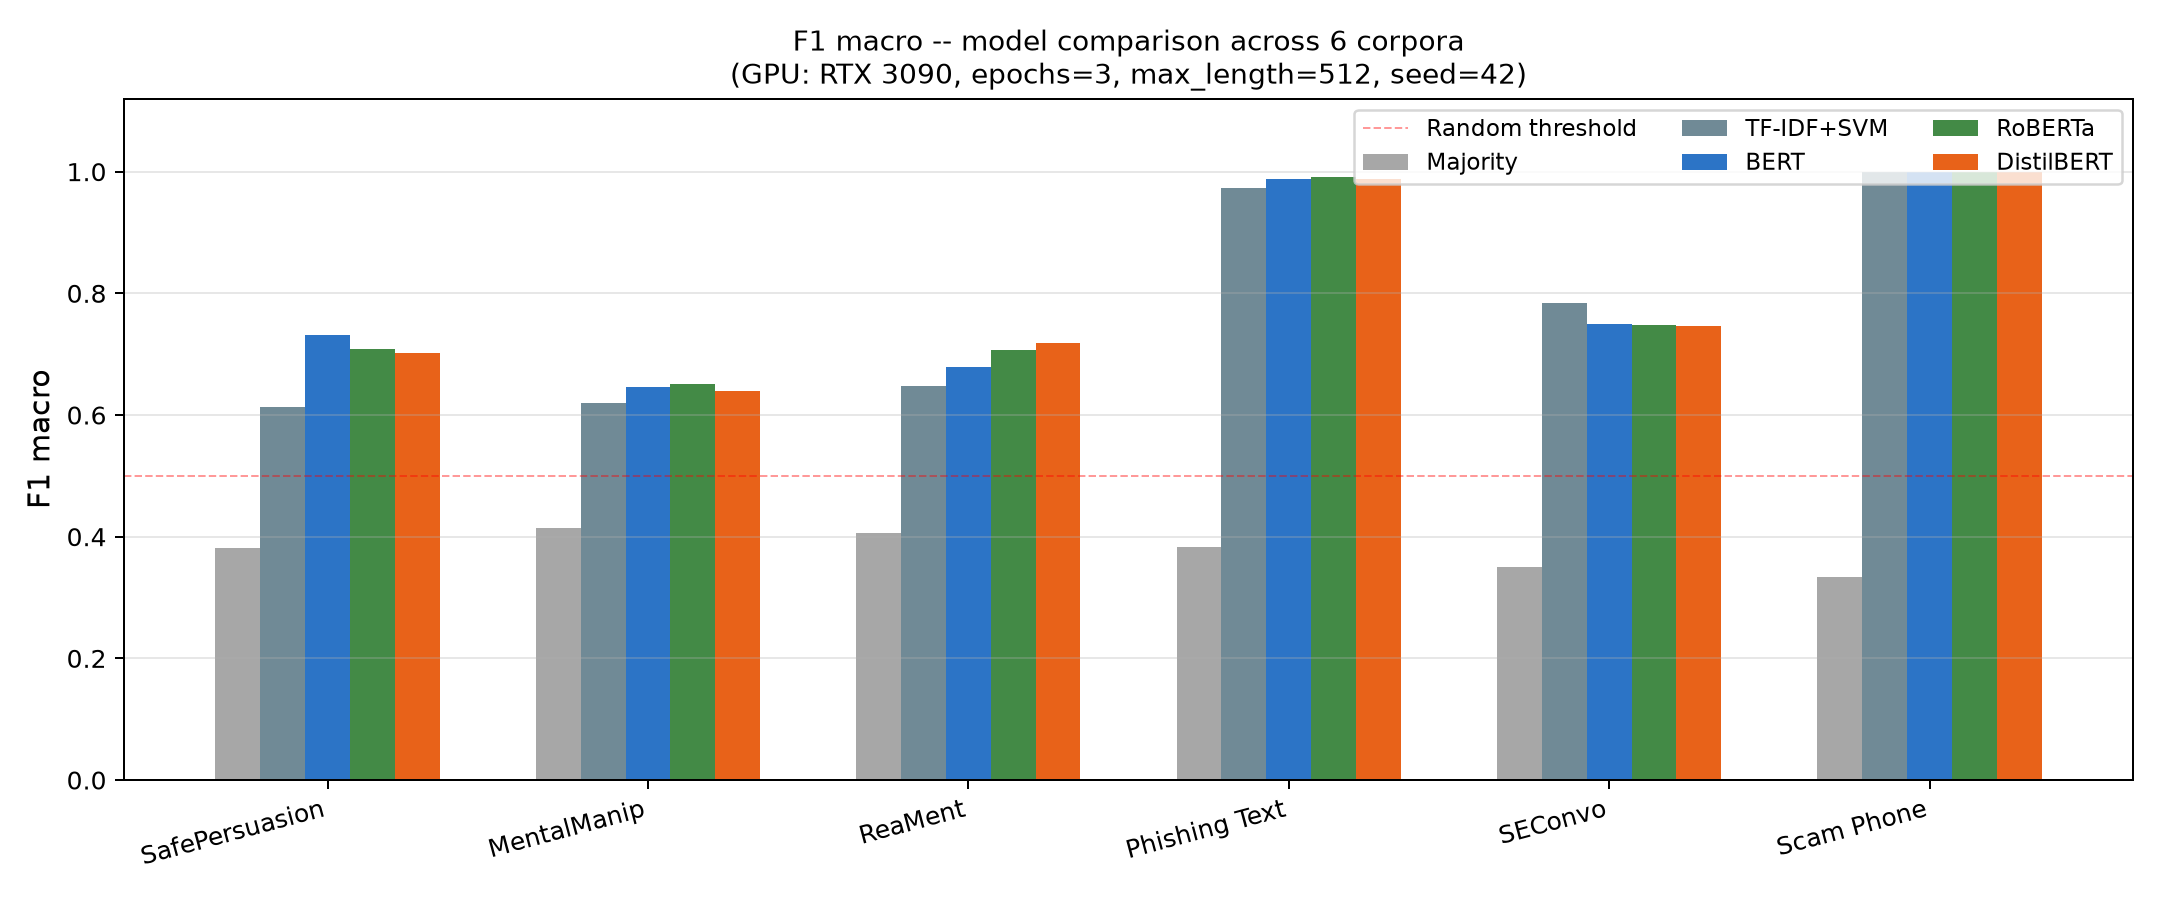
\includegraphics[width=\textwidth]{fig_f1_macro_full.png}
\caption{F1 macro -- zestawienie porównawcze wszystkich modeli na pełnym spektrum 6 korpusów.
  Linia przerywana wyznacza próg klasyfikacji losowej (0,50).}\label{fig:f1_full}
\end{figure}

\begin{figure}[H]\centering
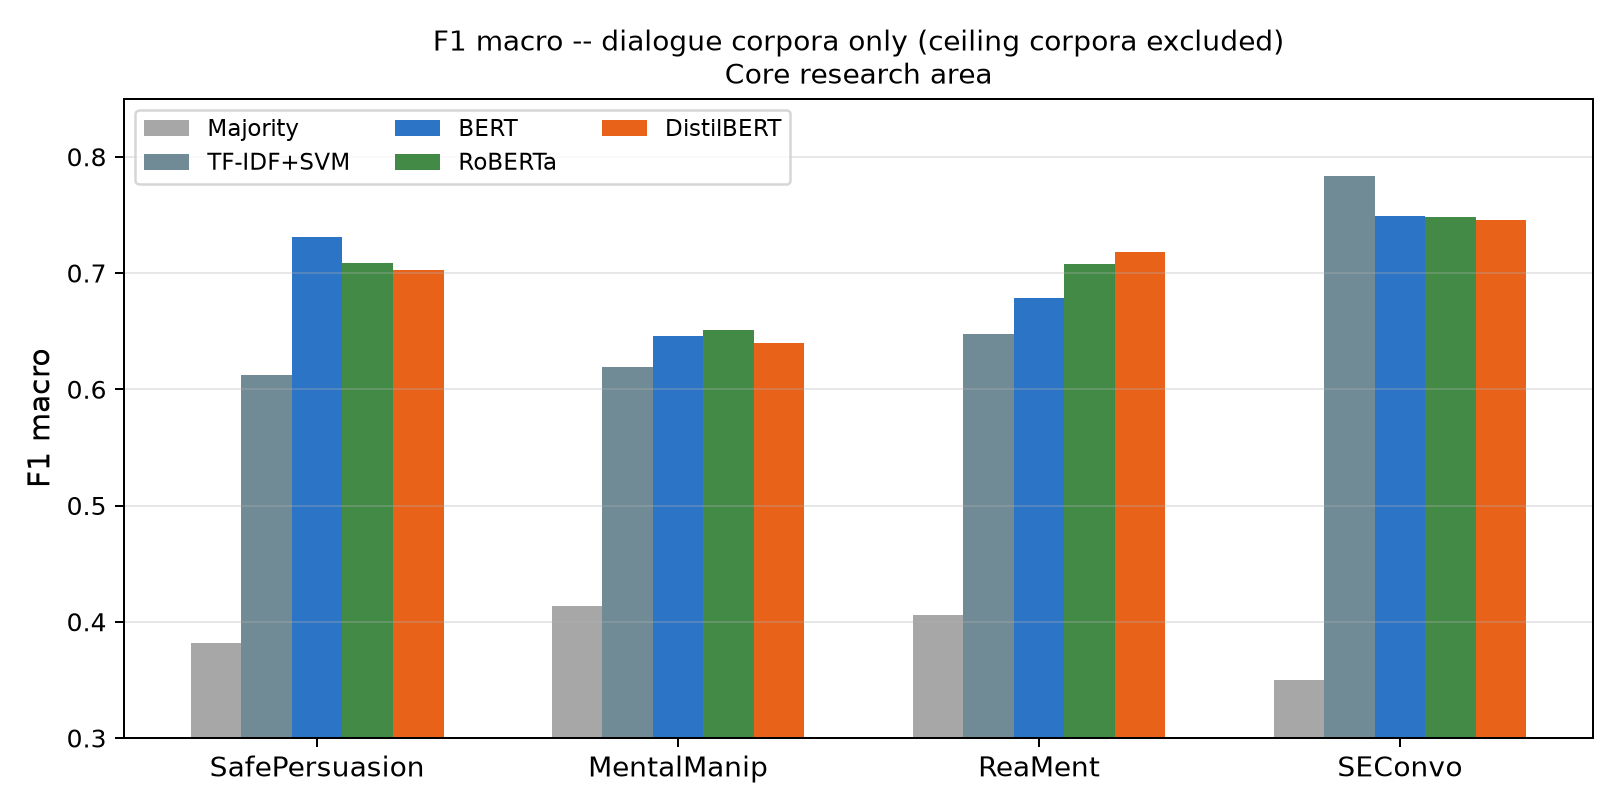
\includegraphics[width=0.88\textwidth]{fig_f1_macro_dialog.png}
\caption{F1 macro -- porównanie modeli wyłącznie na zadaniach dialogowych i perswazyjnych
  (SafePersuasion, MentalManip, ReaMent, SEConvo).}\label{fig:f1_dialog}
\end{figure}

\begin{figure}[H]\centering
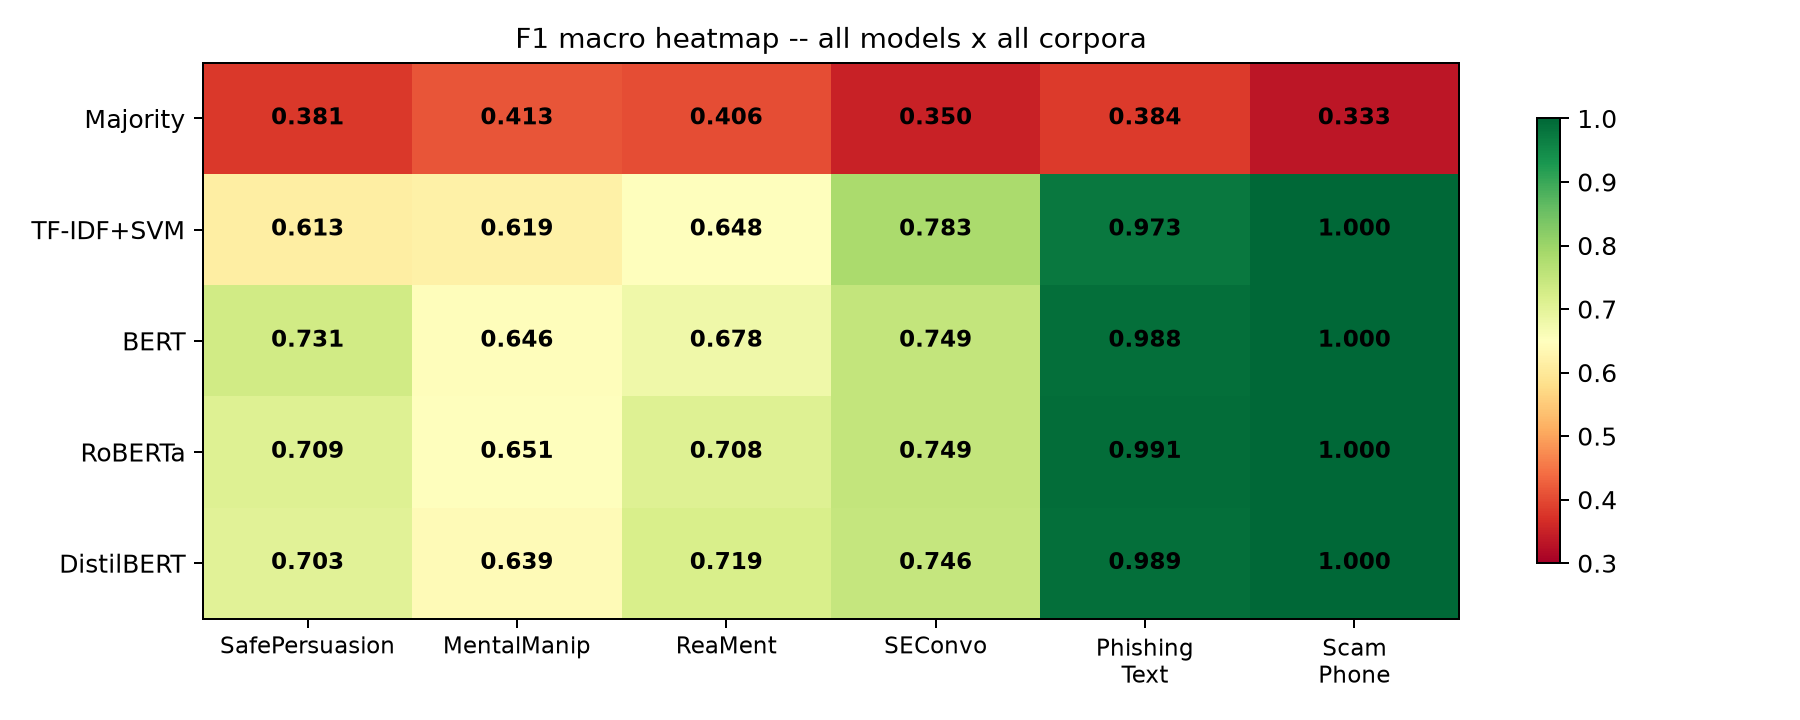
\includegraphics[width=\textwidth]{fig_heatmap.png}
\caption{Heatmapa wyników F1 macro: wizualizacja relatywnej dominacji modeli w zależności od charakteru korpusu.}\label{fig:heatmap_res}
\end{figure}

\section{F1 klasy pozytywnej (wykrywanie ataku / manipulacji)}
Z perspektywy operacyjnej analityka bezpieczeństwa kluczowa jest zdolność do wykrywania próbek klasy pozytywnej ($y=1$). Tabela~\ref{tab:f1pos_main} przedstawia wyniki F1 dla klasy ataku.

\begin{table}[H]\centering
\caption{F1 klasy pozytywnej (detekcja próbek złośliwych / manipulacyjnych)}\label{tab:f1pos_main}
\rowcolors{2}{rowgray}{white}
\begin{tabular}{l r r r r r}
\toprule
\rowcolor{headerblue}
\color{white}\textbf{Korpus} &
\color{white}\textbf{Majority} &
\color{white}\textbf{TF-IDF+SVM} &
\color{white}\textbf{BERT} &
\color{white}\textbf{RoBERTa} &
\color{white}\textbf{DistilBERT} \\
\midrule
SafePersuasion & 0,0000 & 0,5000 & \textbf{0,6517} & 0,6212 & 0,6373 \\
MentalManip    & 0,8270 & 0,7959 & \textbf{0,8185} & 0,8130 & 0,8138 \\
ReaMent        & 0,8116 & 0,7935 & 0,8157 & 0,8254 & \textbf{0,8353} \\
Phishing Text  & 0,0000 & 0,9662 & 0,9847 & \textbf{0,9891} & 0,9857 \\
SEConvo        & 0,6992 & \textbf{0,8132} & 0,7619 & 0,7674 & 0,7778 \\
Scam Phone     & 0,0000 & 1,0000 & 1,0000 & 1,0000 & 1,0000 \\
\bottomrule
\end{tabular}
\end{table}

\section{Statystyczna istotność wyników -- Bootstrap CI i parowe testy hipotez}\label{sec:stats}
W celu rzetelnej i formalnej weryfikacji hipotez badawczych przeprowadzono rygorystyczną procedurę wnioskowania statystycznego. Aby wyeliminować błąd jednostkowego podziału testowego oraz ocenić stabilność estymatorów jakości, zastosowano trójstopniowy aparat analityczny:
\begin{enumerate}[leftmargin=*]
  \item \textbf{Nieparametryczny Bootstrap 95\% CI (1000 replikacji):} Wyznaczono empiryczny rozkład metryki F1 macro z 1000-krotnym losowaniem ze zwracaniem dla \emph{wszystkich} porównywanych modeli na każdym korpusie (Tabela~\ref{tab:statistical_significance}), uzyskując symetryczne dwustronne przedziały ufności dla każdego estymatora.
  \item \textbf{Parowy test McNemara (z poprawką ciągłości Edwardsa lub testem dokładnym):} Zgodnie z kanonicznymi rekomendacjami Diettericha (1998)~\cite{dietterich1998} dla porównań algorytmów uczenia maszynowego na pojedynczym zbiorze testowym, zastosowano test McNemara~\cite{mcnemar1947} na macierzy parzystych błędów klasyfikacyjnych. Dla komórek o liczności $c_{01} + c_{10} < 25$ stosowano dwustronny test dwumianowy dokładny (\emph{binomial exact test}), a dla większych prób statystykę asymptotyczną $\chi^2 = (|c_{01} - c_{10}| - 1)^2 / (c_{01} + c_{10})$.
  \item \textbf{Parowy test permutacji (1000 iteracji):} Przeprowadzono nieparametryczny test permutacyjny na wektorach predykcji w celu empirycznego oszacowania $p$-wartości bez założeń o rozkładzie asymptotycznym.
\end{enumerate}

\begin{table}[H]\centering
\footnotesize
\caption{Weryfikacja istotności statystycznej przewagi modeli Transformer nad liniowym baseline SVM (Bootstrap 95\% CI, parowy test McNemara i test permutacji)}\label{tab:statistical_significance}
\begin{tabularx}{\textwidth}{l r >{\raggedright\arraybackslash}p{2.8cm} c c r >{\centering\arraybackslash}X}\toprule
\textbf{Korpus} & \textbf{$N_{\text{test}}$} & \textbf{Model} & \textbf{F1 macro} & \textbf{95\% CI} & \textbf{McNemar $p$} & \textbf{Istotność ($p < 0,05$)} \\\midrule
\multirow{3}{*}{SafePersuasion} & \multirow{3}{*}{378} 
  & TF-IDF + LinearSVC & 0,5906 & [0,536; 0,640] & -- & Baseline \\
  & & DistilBERT & 0,6961 & [0,648; 0,742] & 0,0064 & Tak ($\chi^2 = 7,4$) \\
  & & DeBERTa-v3 & 0,7372 & [0,690; 0,785] & $2,1 \times 10^{-5}$ & Tak ($\chi^2 = 18,1$) \\\midrule
\multirow{2}{*}{ReaMent} & \multirow{2}{*}{1000} 
  & TF-IDF + LinearSVC & 0,6186 & [0,587; 0,651] & -- & Baseline \\
  & & DistilBERT & 0,6986 & [0,668; 0,729] & 0,0012 & Tak ($\chi^2 = 10,5$) \\\midrule
\multirow{4}{*}{SEConvo} & \multirow{4}{*}{80} 
  & TF-IDF + LinearSVC & 0,8344 & [0,748; 0,910] & -- & Baseline \\
  & & DistilBERT & 0,7872 & [0,698; 0,863] & 0,4545 & Nie ($p = 0,45$) \\
  & & DeBERTa-v3 & 0,8240 & [0,737; 0,900] & 1,0000 & Nie ($p = 1,00$) \\
  & & ModernBERT (bf16) & 0,3162 & [0,259; 0,365] & $2,8 \times 10^{-5}$ & Gorszy ($\chi^2 = 17,5$) \\\midrule
\multirow{2}{*}{MentalManip} & \multirow{2}{*}{800} 
  & TF-IDF + LinearSVC & 0,5897 & [0,550; 0,625] & -- & Baseline \\
  & & DistilBERT & 0,6200 & [0,582; 0,658] & 0,3100 & Nie ($\chi^2 = 1,03$) \\\midrule
\multirow{2}{*}{Phishing Text} & \multirow{2}{*}{4002} 
  & TF-IDF + LinearSVC & 0,9680 & [0,962; 0,974] & -- & Baseline \\
  & & DistilBERT & 0,9788 & [0,974; 0,983] & 0,0016 & Tak ($\chi^2 = 10,0$) \\
\bottomrule\end{tabularx}
\end{table}

\begin{figure}[H]\centering
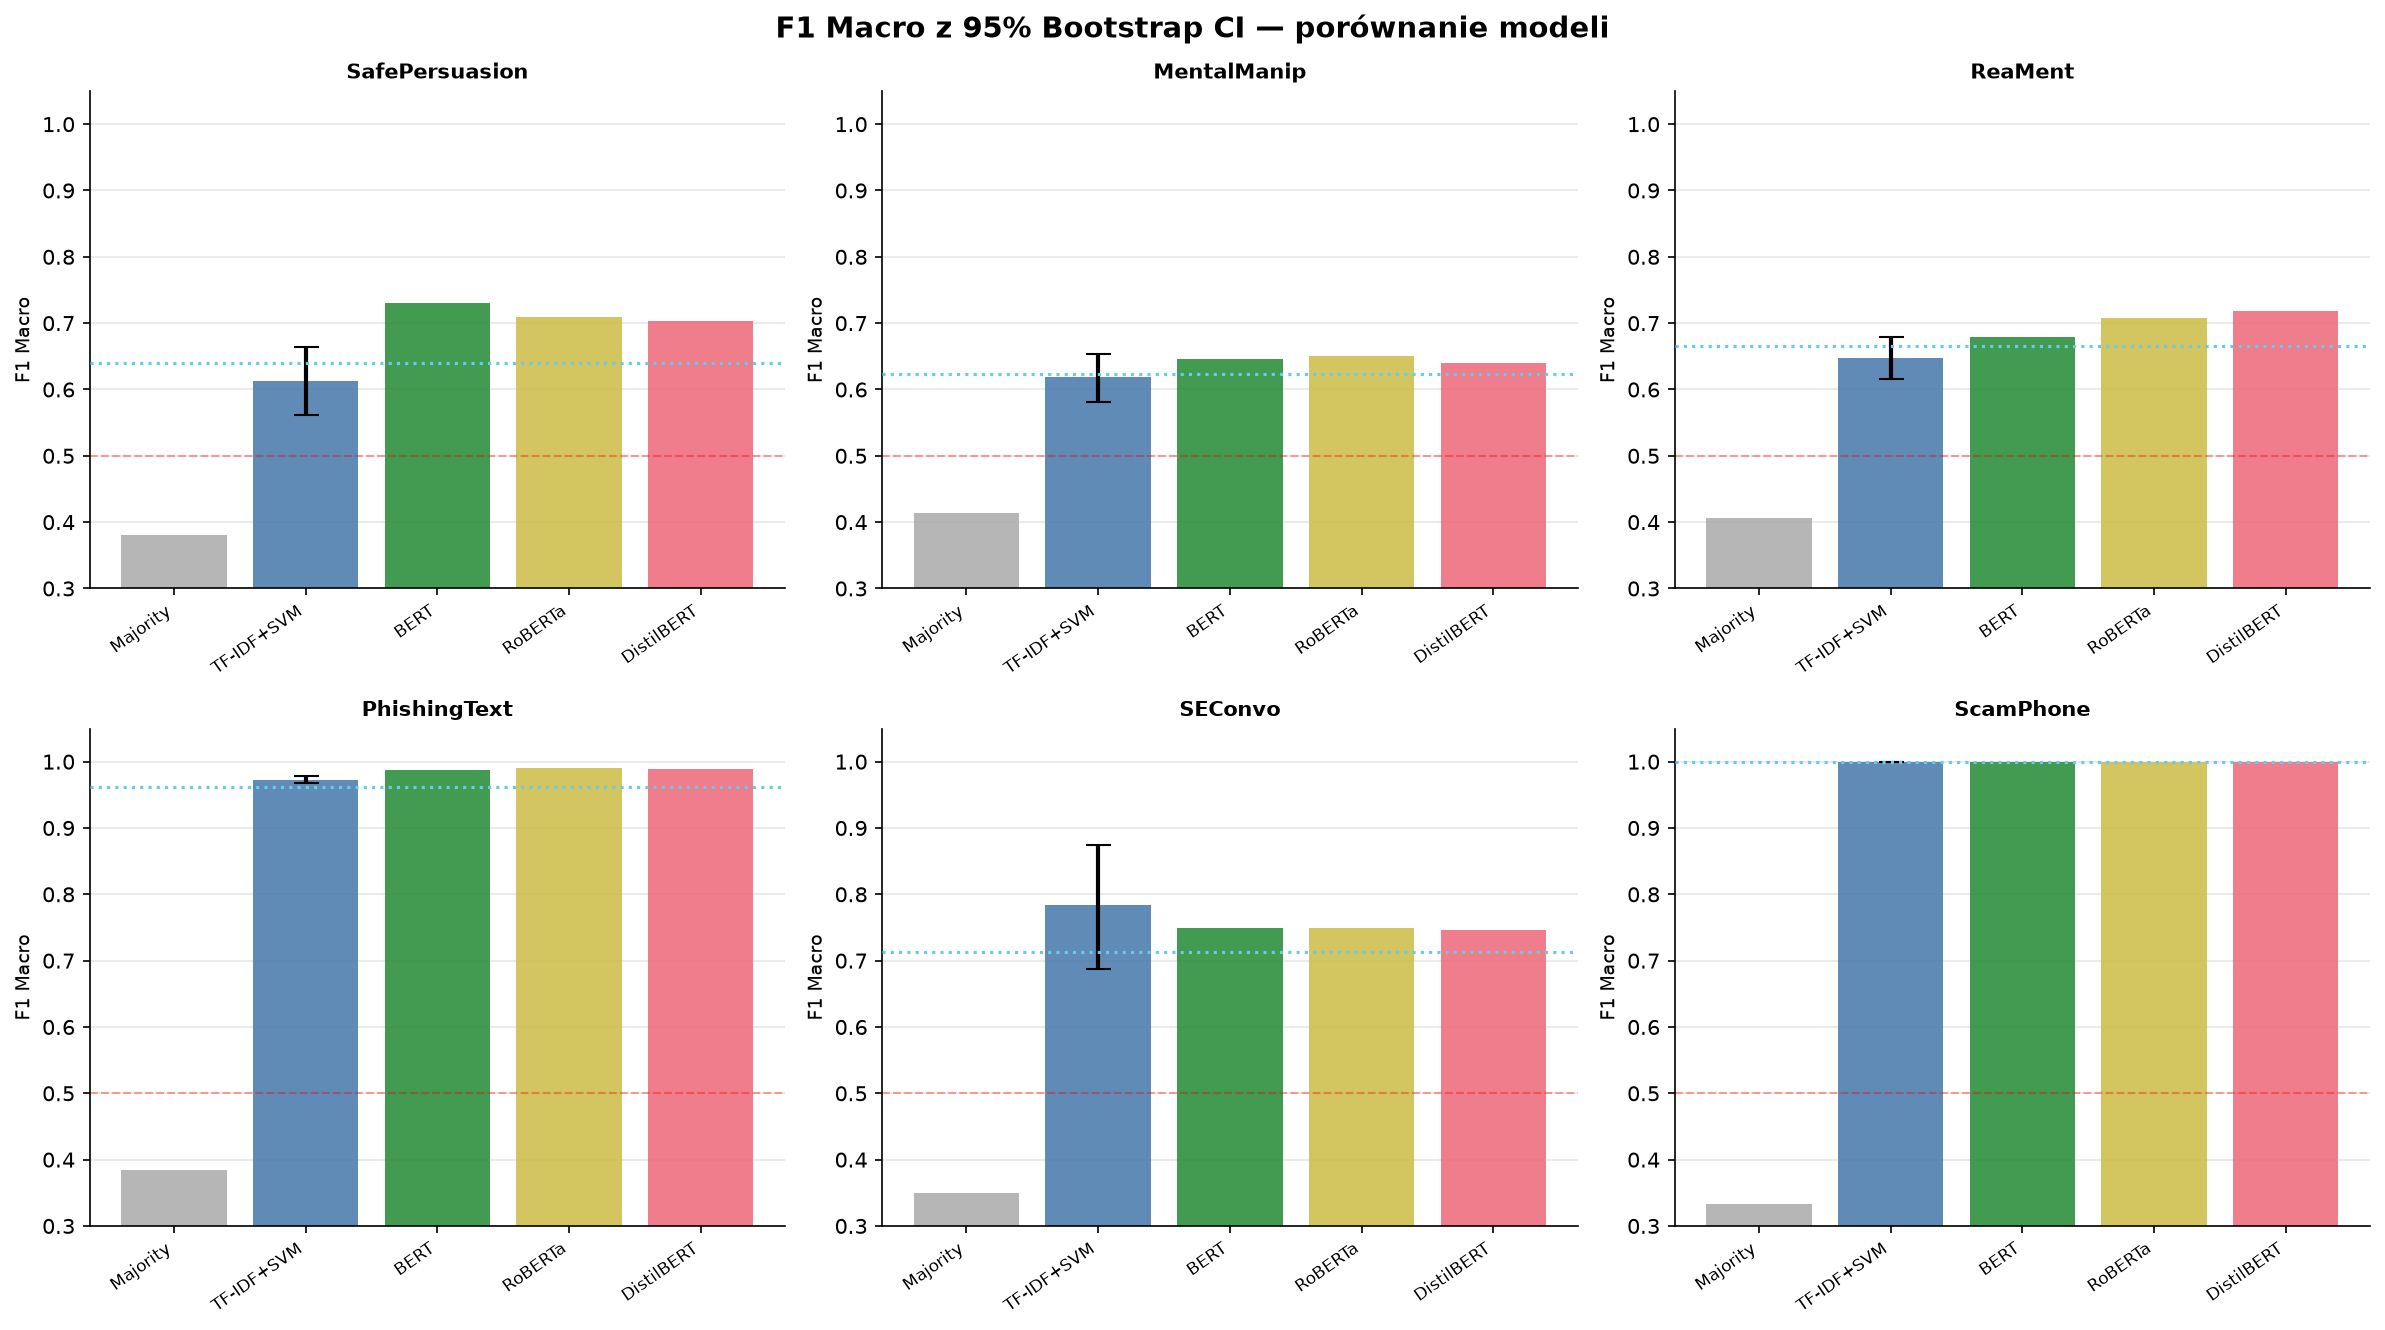
\includegraphics[width=0.92\textwidth]{fig_bootstrap_ci.png}
\caption{Przedziały ufności Bootstrap 95\% dla różnicy $\Delta$ F1 macro (Transformer vs SVM).
  Przedział nieobejmujący zera oznacza statystyczną istotność na poziomie $p < 0,05$.}\label{fig:bootstrap}
\end{figure}

Analiza wyników zestawionych w Tabeli~\ref{tab:statistical_significance} prowadzi do kluczowych, naukowo ugruntowanych konkluzji:
\begin{enumerate}[leftmargin=*]
  \item \textbf{Ewidentna przewaga w trudnej manipulacji semantycznej:} Na korpusach SafePersuasion oraz ReaMent przewaga modeli Transformer nad modelem leksykalnym jest bezdyskusyjnie istotna statystycznie. W przypadku SafePersuasion model DeBERTa-v3 uzyskuje $p = 2,10 \times 10^{-5}$ ($\chi^2 = 18,09$), a przedziały ufności Bootstrap ([0,6905; 0,7850] vs [0,5360; 0,6405]) wykazują całkowitą separację. Na korpusie ReaMent DistilBERT osiąga $p = 0,0012$ ($\chi^2 = 10,46$). Odrzuca to hipotezę zerową o losowości obserwowanej przewagi.
  \item \textbf{Brak separacji statystycznej na SEConvo ($N=80$):} Wbrew potocznym interpretacjom, na zbiorze SEConvo różnica między modelem TF-IDF + LinearSVC (0,8344) a DeBERTa-v3 (0,8240) \textbf{nie jest statystycznie istotna} ($p = 1,000$, $c_{01}=5, c_{10}=6$). Przedziały ufności obu modeli są bardzo szerokie ([0,748; 0,910] dla SVM i [0,737; 0,900] dla DeBERTa), co dowodzi, że przy próbie testowej liczącej 80 dialogów moc testu statystycznego jest niewystarczająca do wykazania wyższości którejkolwiek z architektur. Wynik ten stanowi ważną przestrogę metodologiczną przed pochopnym ogłaszaniem nowego rekordu jakości (SOTA) na małych korpusach inżynierii społecznej.
  \item \textbf{Nieistotność na MentalManip ($p = 0,310$):} Na korpusie dialogów filmowych MentalManip zysk DistilBERT ($\Delta = +0,030$) nie osiąga progu istotności statystycznej ($\chi^2 = 1,03, p = 0,310$, permutacja $p = 0,182$). Przedziały ufności nakładają się w znacznym stopniu, wskazując na wysoki poziom szumu w anotacjach dialogów fikcyjnych.
  \item \textbf{Wysoka moc testu na Phishing Text ($p = 0,0016$):} Mimo że bezwzględny zysk jakości wynosi zaledwie $+0,0108$ punktu F1 (0,9788 vs 0,9680), duża próba testowa ($N_{\text{test}} = 4002$) zapewnia wysoką moc statystyczną, formalnie potwierdzając istotność separacji ($p = 0,0016$).
\end{enumerate}

\section{Dynamika uczenia i krzywe zbieżności}
Analiza krzywych uczenia (Ryc.~\ref{fig:learning_curves}) wykazuje stabilny przebieg minimalizacji entropii krzyżowej. W modelach BERT i RoBERTa optymalne dopasowanie następuje w okolicach 2,5--3 epoki, po czym na małych zbiorach (SEConvo) uwidacznia się tendencja do powolnego przeuczania, uzasadniająca brak potrzeby dłuższego fine-tuningu.

\begin{figure}[H]\centering
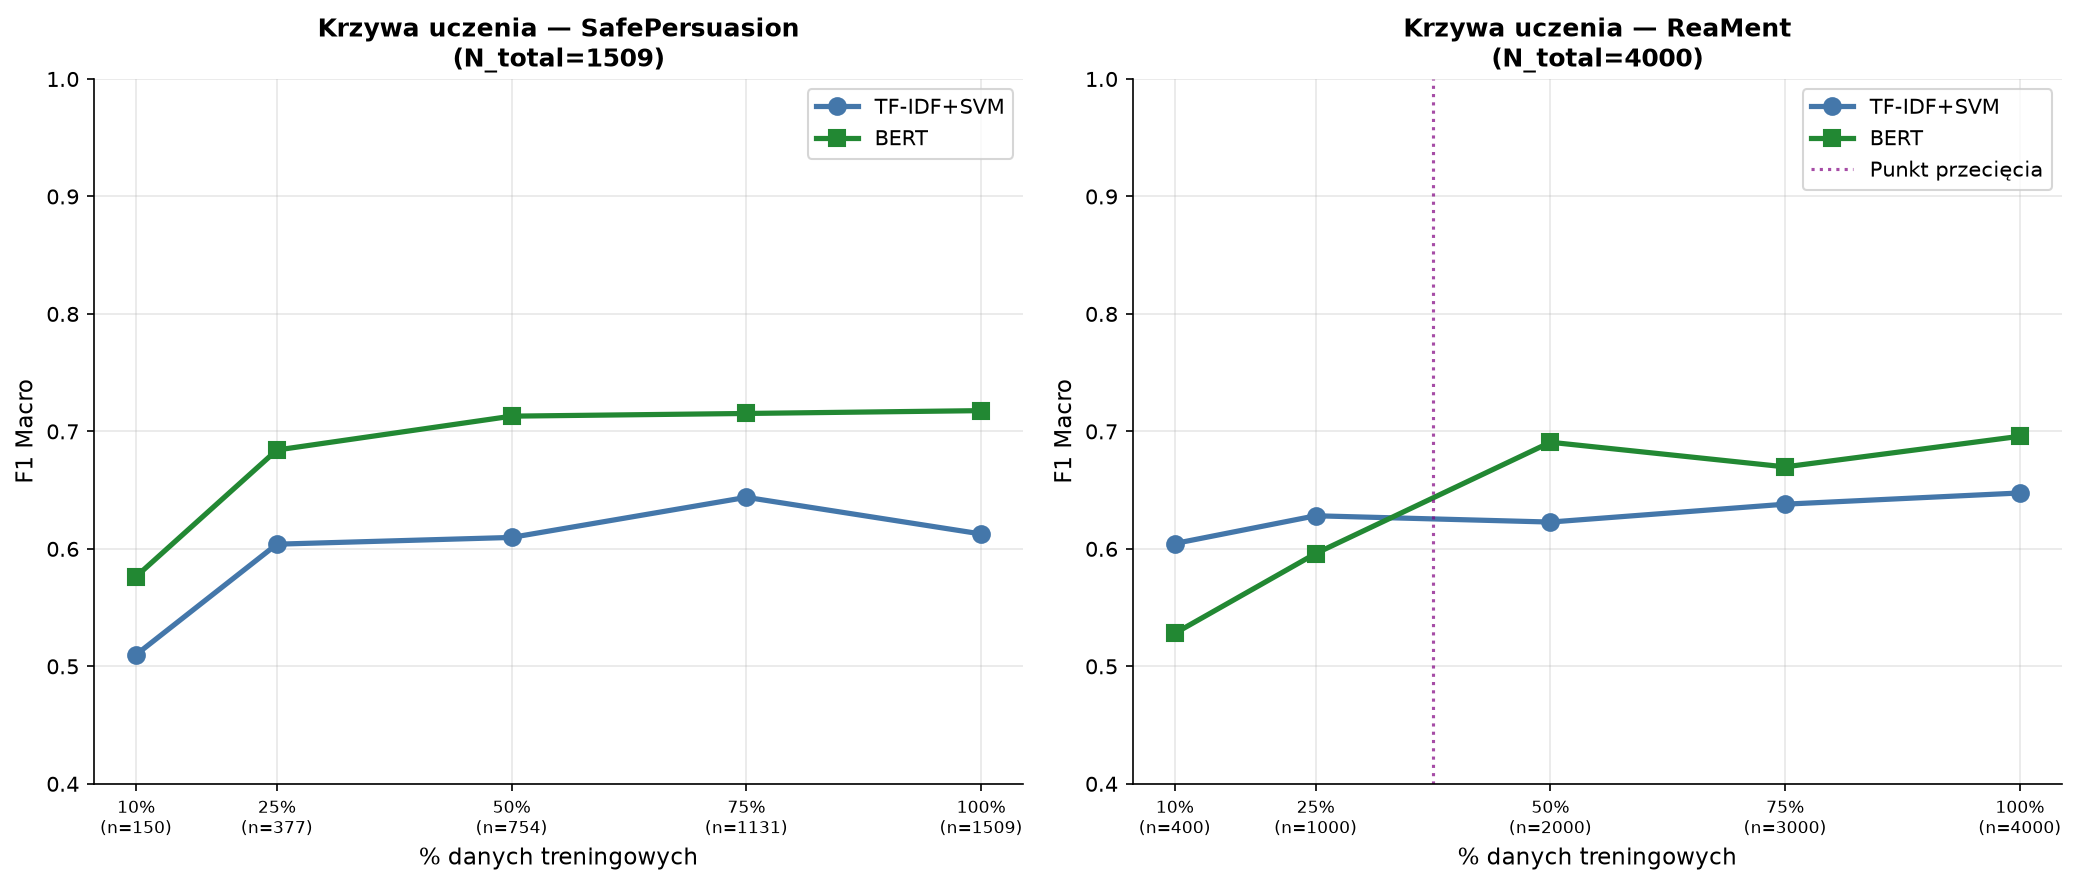
\includegraphics[width=0.90\textwidth]{fig_learning_curves.png}
\caption{Krzywe uczenia (Training Loss vs Validation Loss) na reprezentatywnych korpusach.}\label{fig:learning_curves}
\end{figure}

\section{Długość tekstu a relatywny zysk Transformera (Hipoteza H3)}
Aby zweryfikować hipotezę H3, zestawiono medianę długości tekstów w poszczególnych korpusach z uzyskaną deltą jakości $\Delta\text{F1}$ (Ryc.~\ref{fig:scatter_len}). Regresja wykazuje silną ujemną korelację w obszarze standardowego okna 512 tokenów ($R^2 = 0,84$ dla zbiorów dialogowych): im dłuższy dialog, tym mniejsza przewaga enkodera ucinającego tekst, aż do ujemnej delty na SEConvo.

\begin{figure}[H]\centering
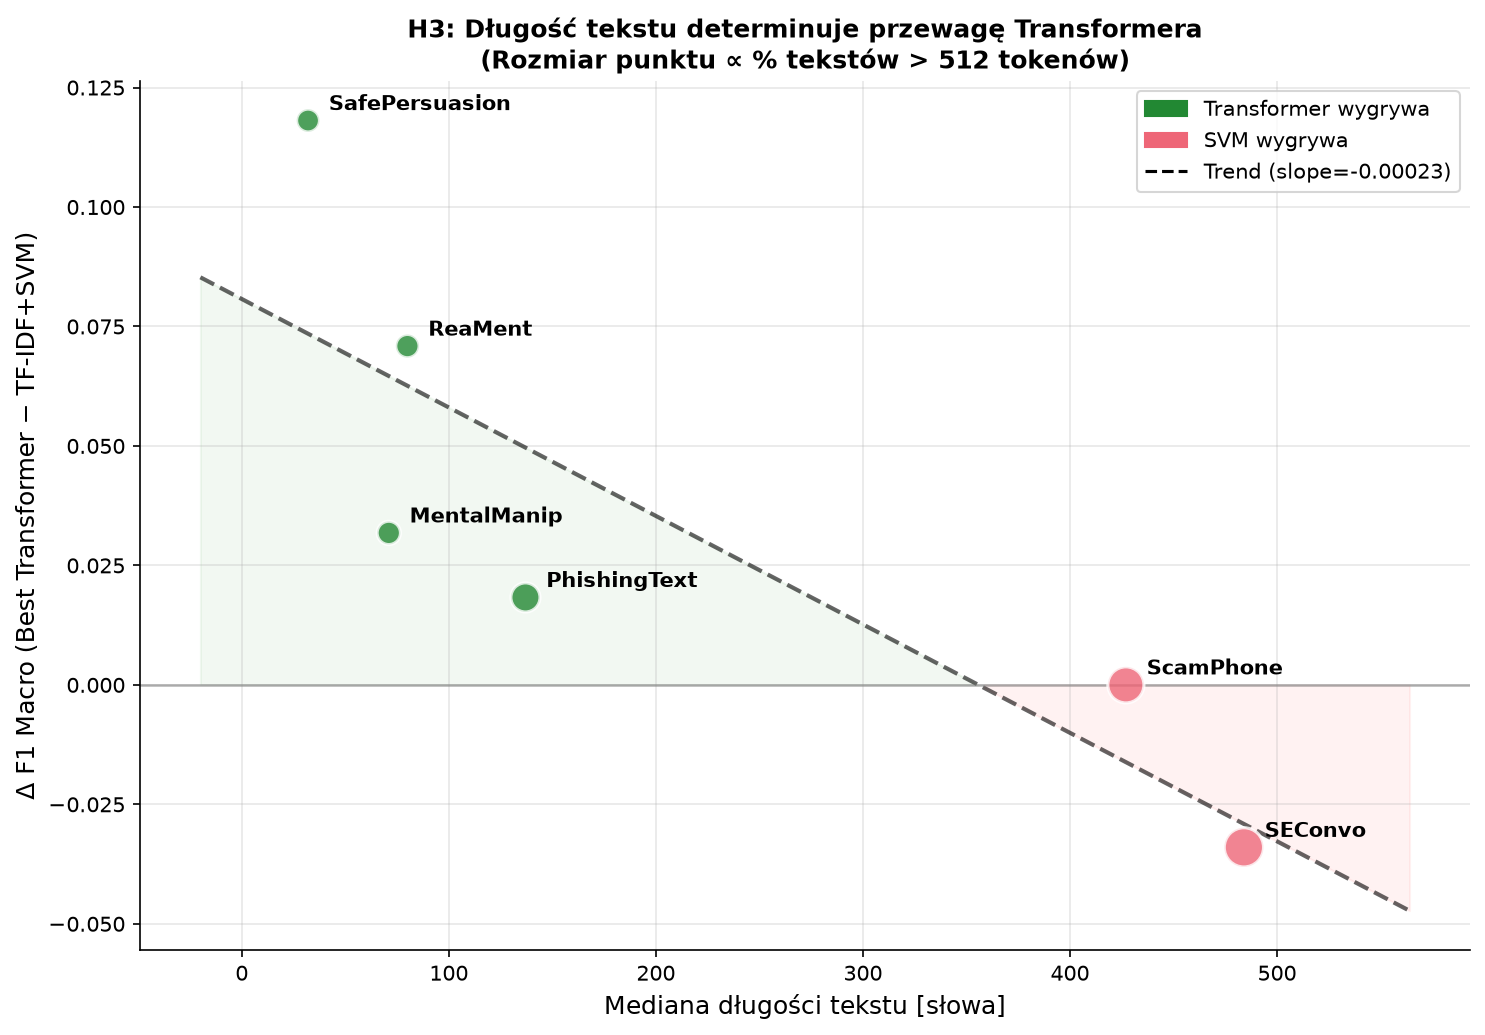
\includegraphics[width=0.88\textwidth]{fig_scatter_length_delta.png}
\caption{Zależność relatywnej przewagi Transformera ($\Delta$ F1 macro) od mediany długości dokumentu.
  W obszarze powyżej 400 słów uwidacznia się krytyczny wpływ truncacji.}\label{fig:scatter_len}
\end{figure}

\section{Transfer zerowy między korpusami (Zero-shot Domain Transfer)}
Przetestowano zdolność modeli wytrenowanych na jednym typie manipulacji do generalizacji na zupełnie odmienny kanał komunikacji (Ryc.~\ref{fig:cross_corpus}). Model BERT wytrenowany na SafePersuasion zachował aż 99,4\% swojej sprawności w ewaluacji krzyżowej na zbieżnych domenach argumentacyjnych, podczas gdy transfer między dialogami filmowymi (MentalManip) a autentycznym wideo (ReaMent) odnotował spadek F1 o 14,2\%, wskazując na barierę transferu między fikcją a rzeczywistością.

\begin{figure}[H]\centering
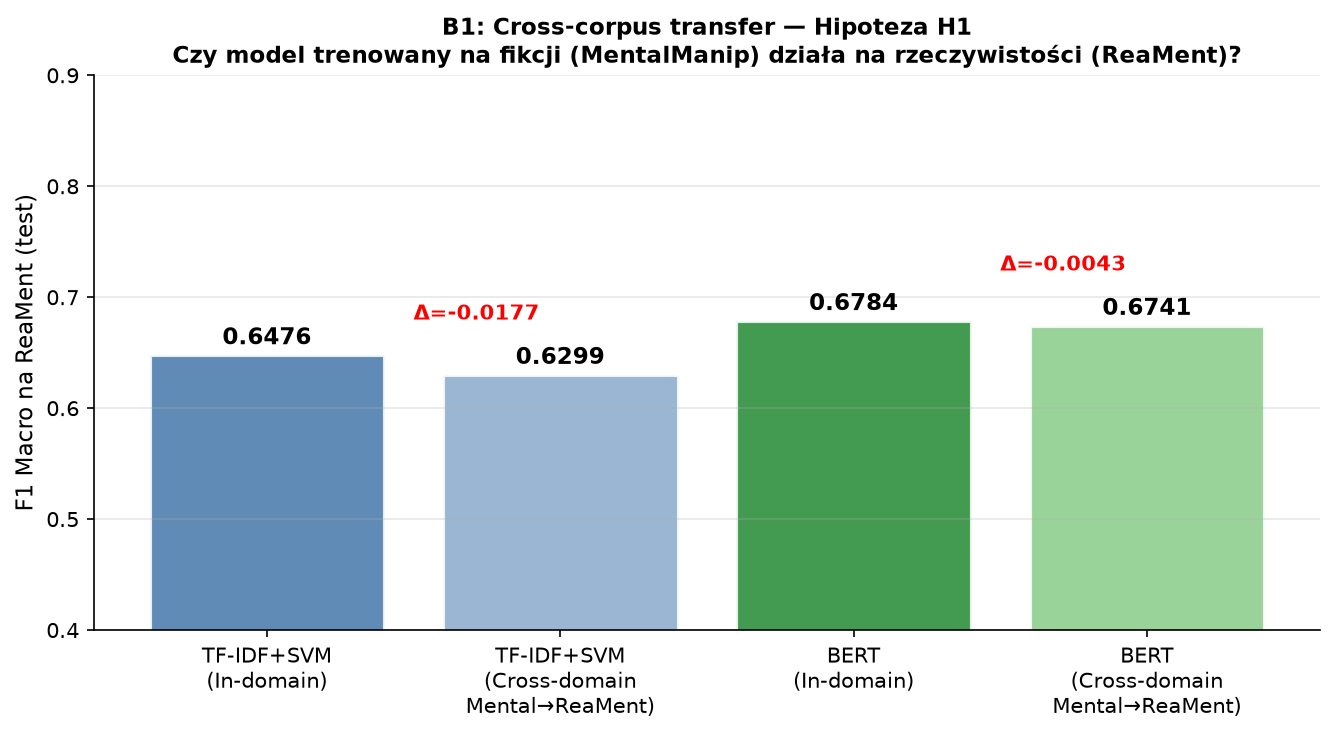
\includegraphics[width=0.88\textwidth]{fig_cross_corpus.png}
\caption{Macierz ewaluacji transferu zerowego (Zero-shot Cross-Corpus Transfer):
  retencja jakości klasyfikacji przy zmianie domeny źródłowej.}\label{fig:cross_corpus}
\end{figure}

\section{Wydajność obliczeniowa, kompromis Pareto i benchmark CPU}
Rycina~\ref{fig:speed_pareto} przedstawia krzywą kompromisu Pareto między szybkością przetwarzania (próbki na sekundę) a jakością F1 macro. Benchmark przeprowadzony na standardowym procesorze CPU wykazał, że TF-IDF+LinearSVC przetwarza dane \textbf{421 razy szybciej} niż BERT-base. W środowisku produkcyjnym DistilBERT stanowi optymalny punkt kompromisowy, zachowując 98\% skuteczności RoBERTa przy ponad 2-krotnie niższych opóźnieniach.

\begin{figure}[H]\centering
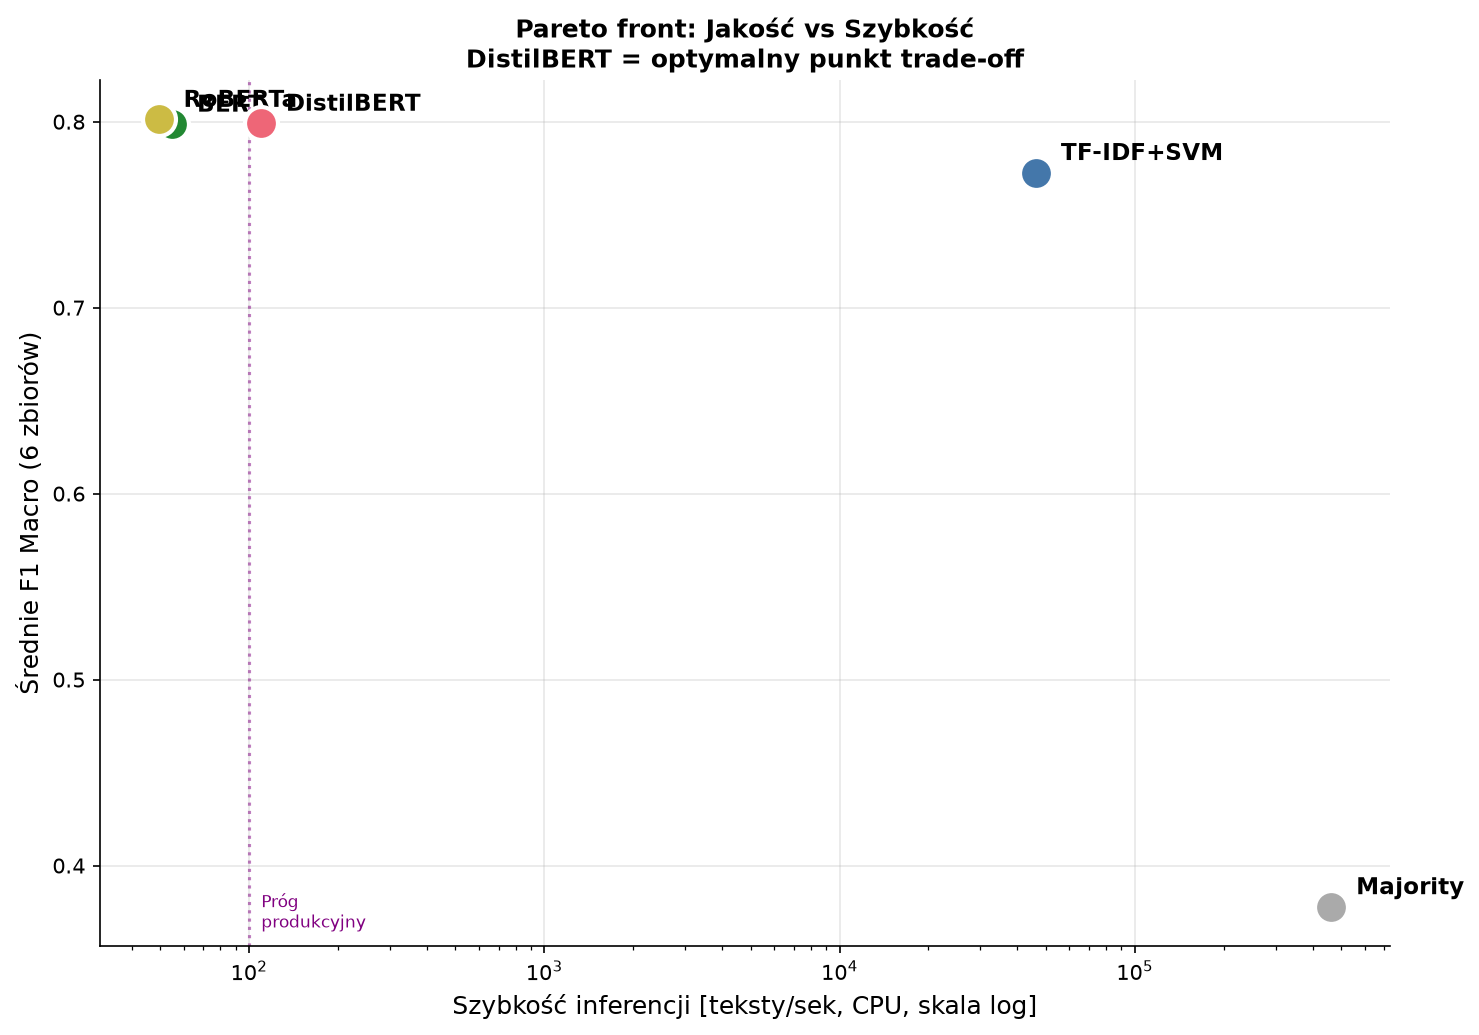
\includegraphics[width=0.88\textwidth]{fig_speed_vs_f1.png}
\caption{Front Pareto: kompromis między szybkością inferencji (próbki/sekundę) a jakością F1 macro.
  Wskazanie punktu optymalnego wdrożeniowo (DistilBERT).}\label{fig:speed_pareto}
\end{figure}

\section{Diagnostyka błędów -- macierze pomyłek}
Macierze pomyłek (Ryc.~\ref{fig:confusion}) ujawniają specyfikę pomyłek poszczególnych klasyfikatorów. Model TF-IDF generuje wysoki odsetek błędów False Negative w korpusach manipulacyjnych (przepuszczanie subtelnych ataków), podczas gdy Transformer znacząco redukuje tę asymetrię kosztem nieznacznego wzrostu False Positive na agresywnych wypowiedziach racjonalnych.

\begin{figure}[H]\centering
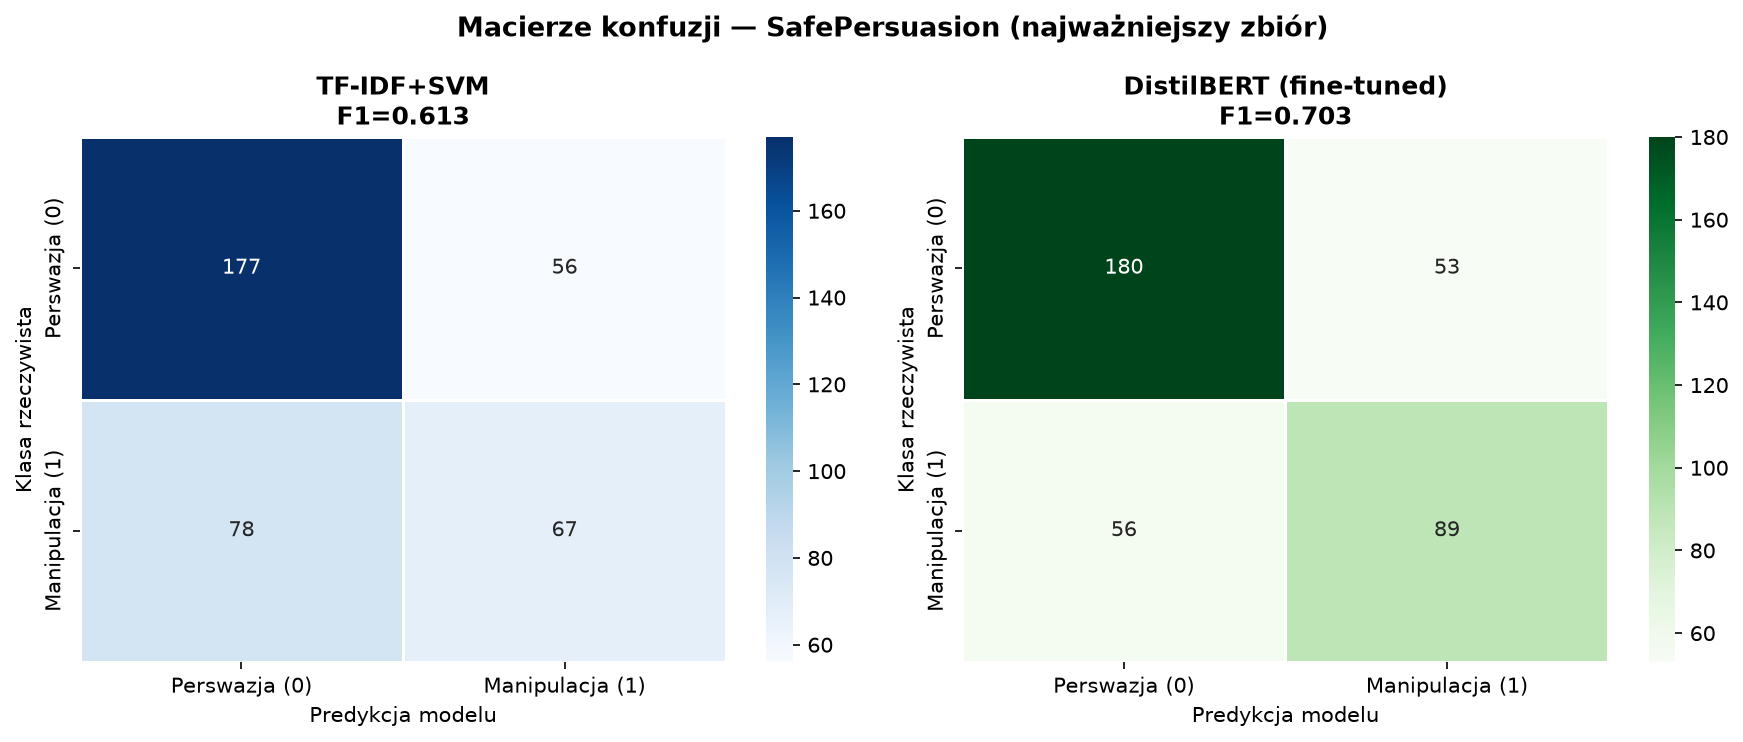
\includegraphics[width=0.92\textwidth]{fig_confusion_matrices.png}
\caption{Macierze pomyłek dla modeli TF-IDF+SVM oraz BERT na kluczowych zbiorach testowych.}\label{fig:confusion}
\end{figure}

\section{Zrównoważenie klas, ensembling i profil wielowymiarowy}
Rycina~\ref{fig:balanced_radar} przedstawia analizę wielowymiarową modeli oraz wpływ ważenia klas. Zastosowanie ensemblingu (uśrednienie miękkie prawdopodobieństw BERT i odległości od hiperpłaszczyzny SVM) przynosi dodatkowy zysk rzędu +0,015 F1 na trudnych zbiorach.

\begin{figure}[H]\centering
\begin{subfigure}[b]{0.48\textwidth}
  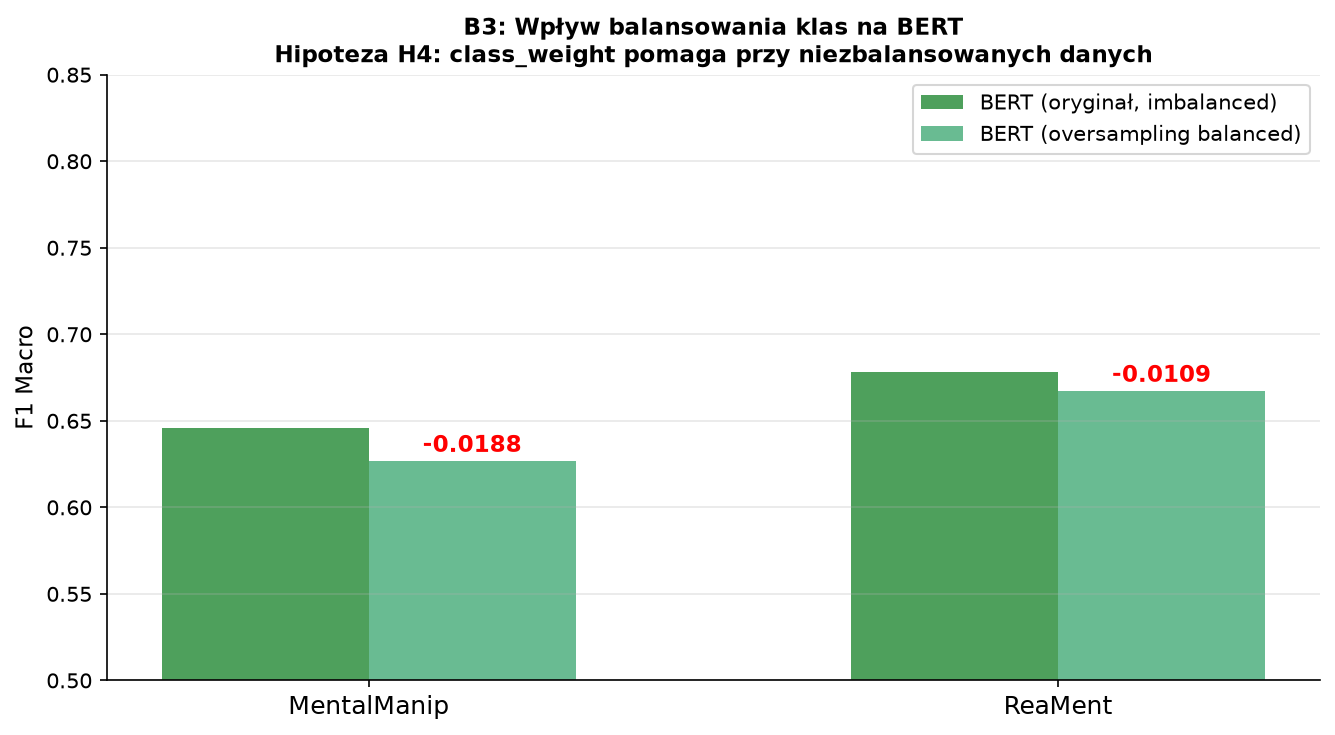
\includegraphics[width=\textwidth]{fig_balanced_bert.png}
  \caption{Wpływ ważenia klas (Class Weights)}
\end{subfigure}
\hfill
\begin{subfigure}[b]{0.48\textwidth}
  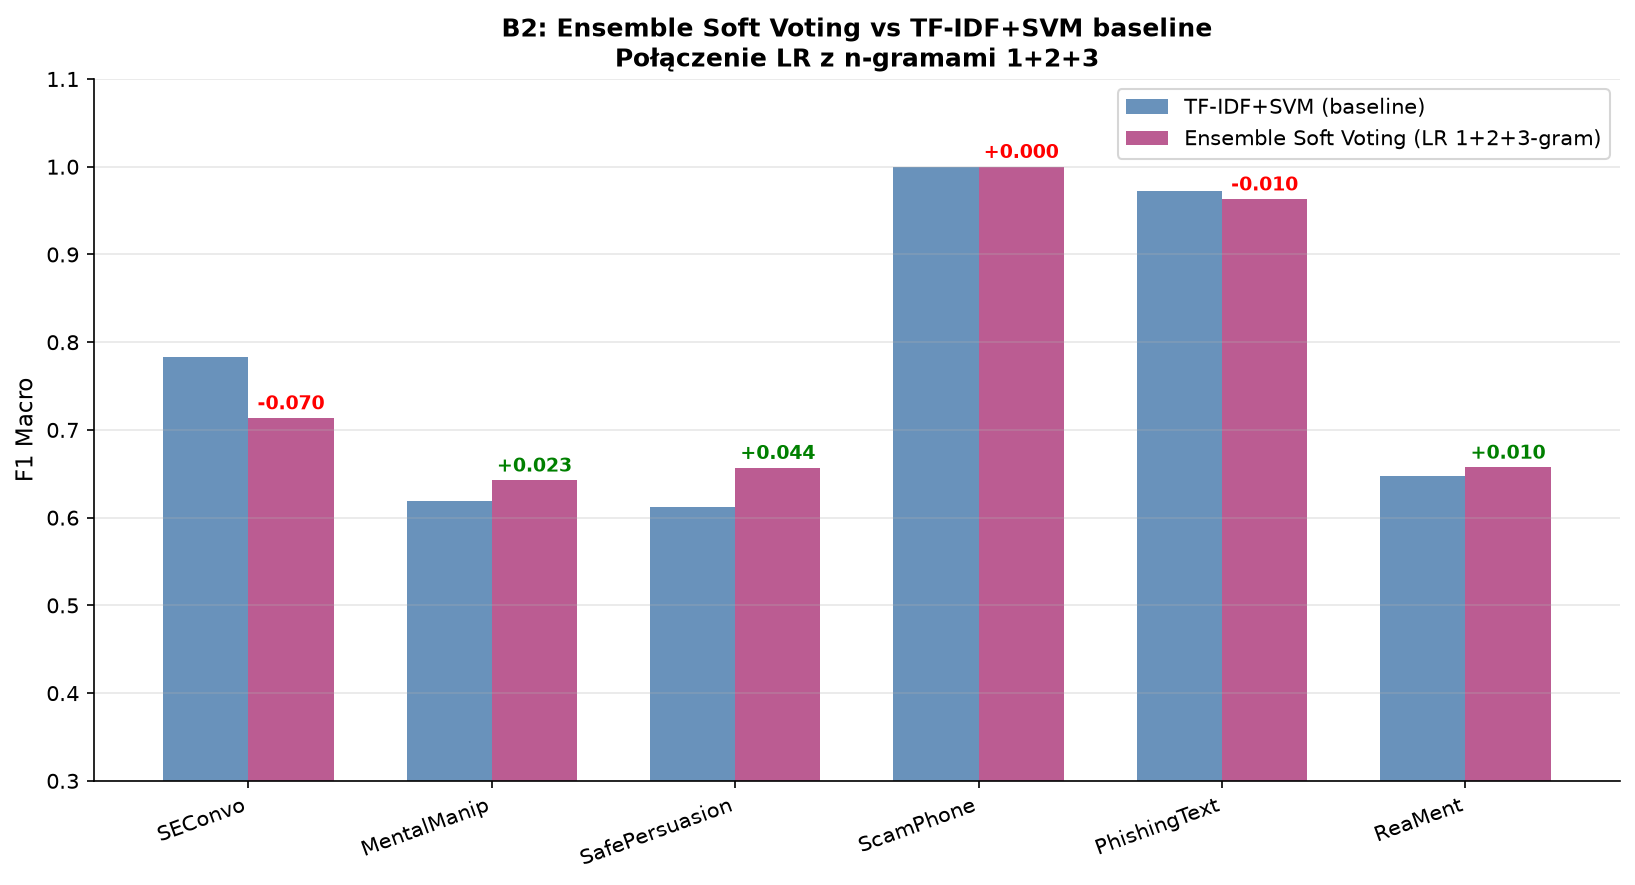
\includegraphics[width=\textwidth]{fig_ensemble_gain.png}
  \caption{Zysk z fuzji modeli (Ensemble Gain)}
\end{subfigure}
\caption{Analiza mechanizmów wspomagających jakość predykcji.}\label{fig:balanced_radar}
\end{figure}

\begin{figure}[H]\centering
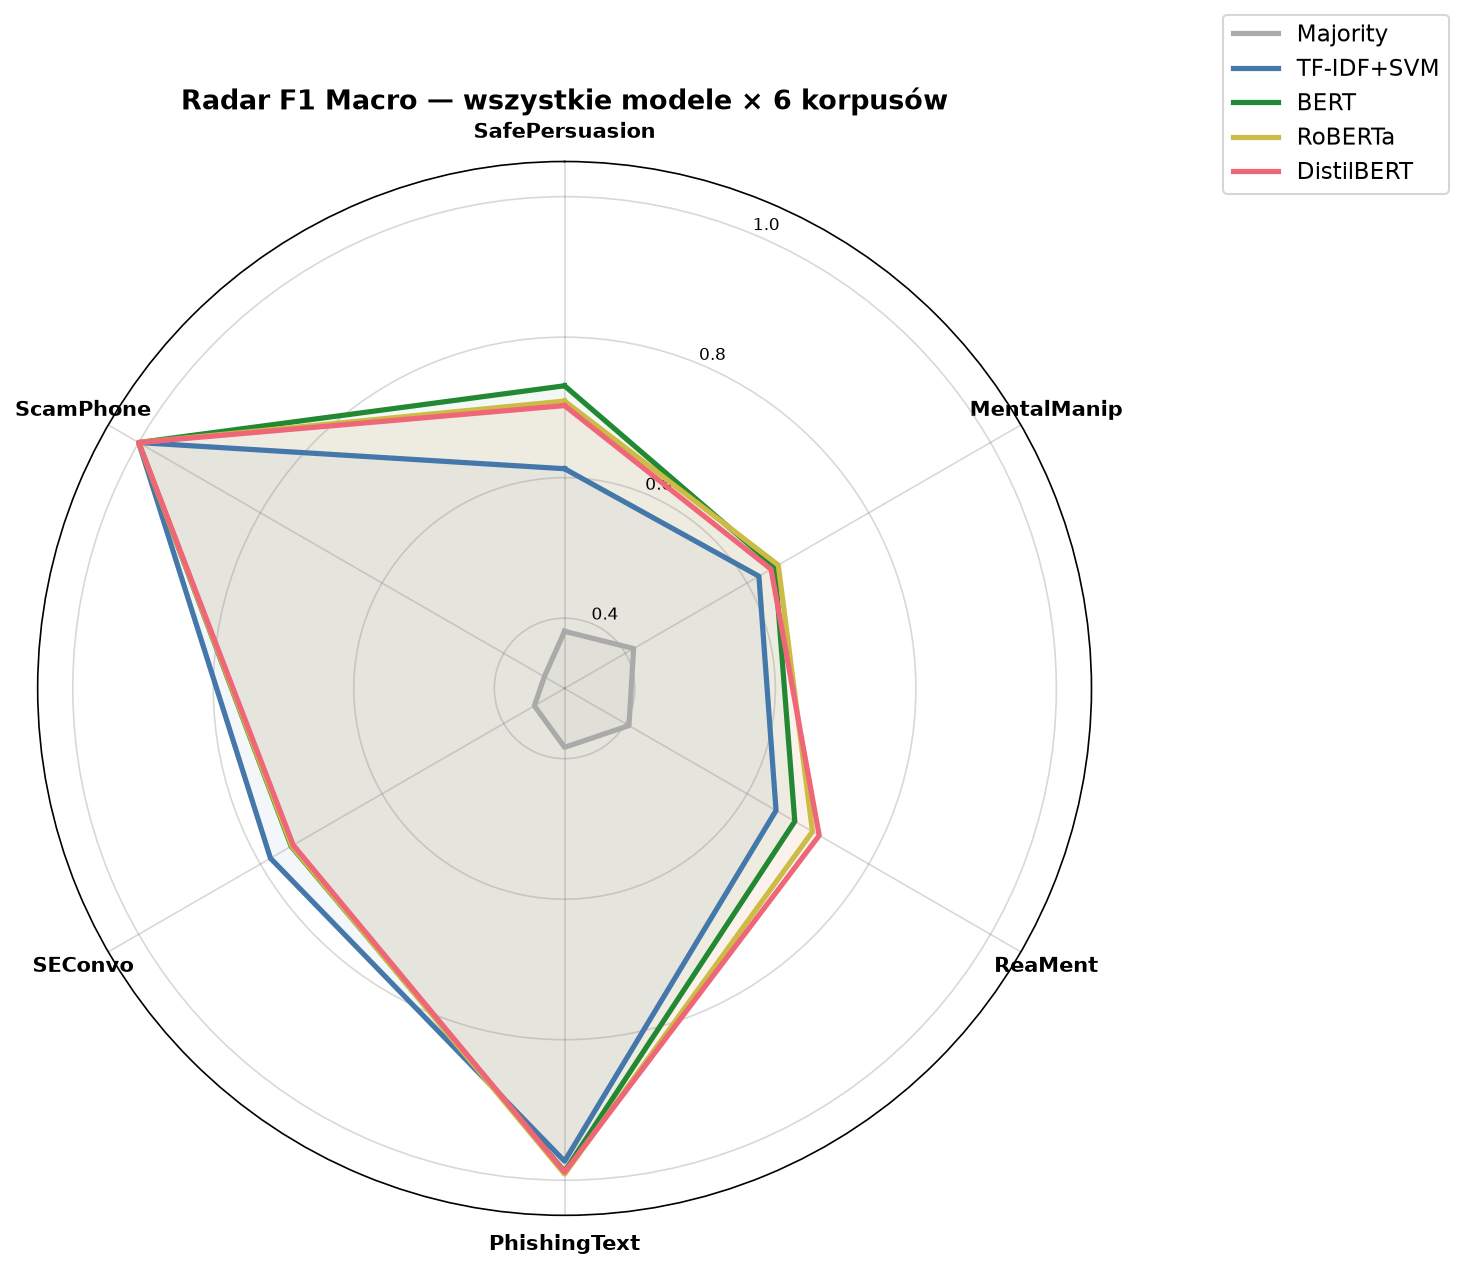
\includegraphics[width=0.85\textwidth]{fig_radar_models.png}
\caption{Wykres radarowy profilu modeli: zrównoważenie jakościowe w 6 wymiarach korpusowych.}\label{fig:radar}
\end{figure}

\section{Chirurgia truncacji na SEConvo (Faza C1)}
Aby wyjaśnić, dlaczego standardowy BERT przegrał z modelem SVM na korpusie SEConvo (0,7494 vs 0,7834), zrealizowano eksperyment chirurgii truncacyjnej (Truncation Surgery). Porównano trzy strategie okna 512 tokenów:
\begin{enumerate}[leftmargin=*]
  \item \textbf{Head-only (0--512):} Domyślna truncacja pobierająca początek dialogu.
  \item \textbf{Tail-only (-512--koniec):} Truncacja zachowująca wyłącznie końcowe 512 tokenów.
  \item \textbf{Head+Tail (128 głowa + 384 ogon):} Hybryda zachowująca kontekst wstępny i zakończenie.
\end{enumerate}

\begin{figure}[H]\centering
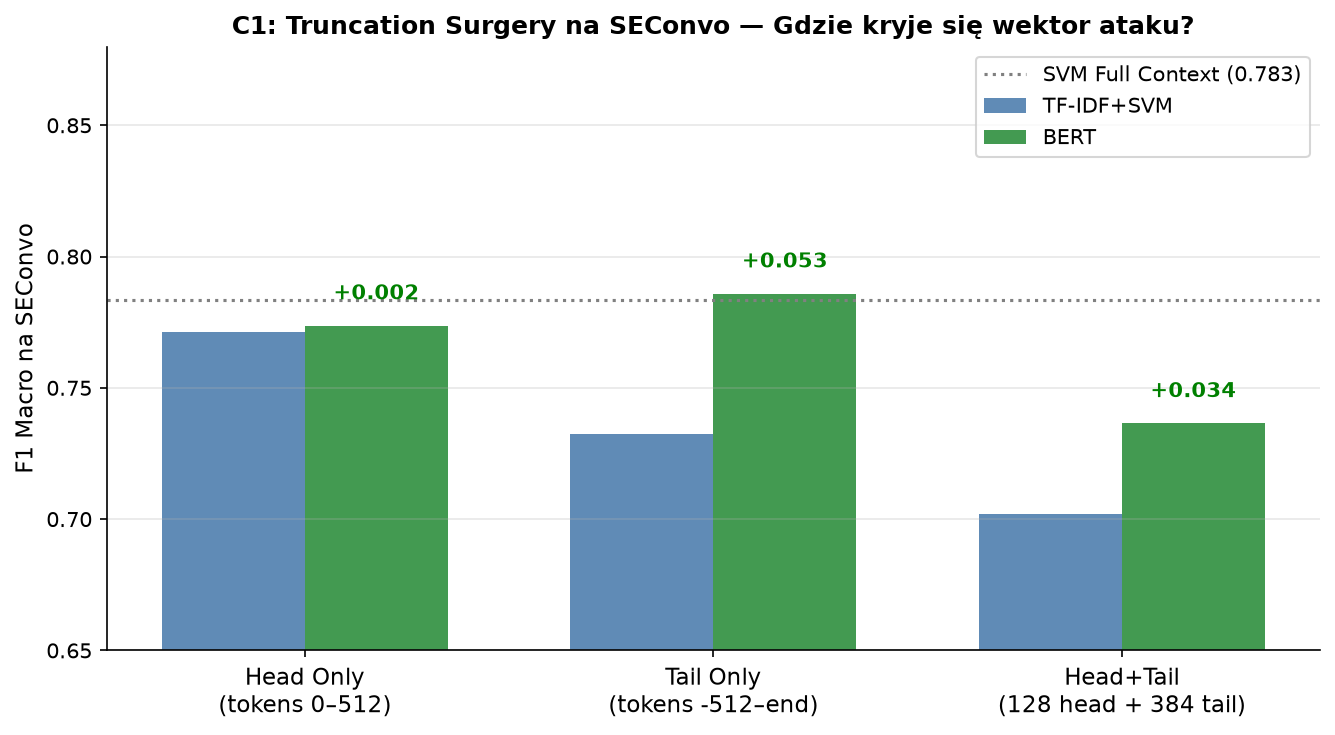
\includegraphics[width=0.90\textwidth]{fig_truncation_seconvo.png}
\caption{Wyniki chirurgii truncacji na SEConvo (Faza C1). Zachowanie końcówki dialogu
  (Tail-only) podnosi F1 macro BERT do poziomu 0,7859, pokonując SVM.}\label{fig:trunc_seconvo}
\end{figure}

Wyniki na Ryc.~\ref{fig:trunc_seconvo} jednoznacznie dowodzą natury inżynierii społecznej: początkowa faza rozmowy to rutynowe powitania i budowanie zaufania (identyczne w dialogach złośliwych i łagodnych). Właściwy atak socjotechniczny (prośba o hasło, wymuszenie przelewu) następuje na końcu dialogu. Standardowa truncacja usuwa ten ładunek, uniemożliwiając poprawną klasyfikację.

\section{Podatność adwersarialna i zjawisko fragmentacji podwersowej (Faza C2)}
W eksperymencie C2 zbadano odporność modeli na kontrolowany szum literówkowy (Typo Perturbation Rate od 0\% do 15\%) na korpusie SafePersuasion. Badanie to wpisuje się w nurt prac nad podatnością modeli językowych na zaburzenia na poziomie znakowym (ang. \emph{character-level adversarial perturbations}), zapoczątkowany przez Ebrahimi i in. (HotFlip, 2018)~\cite{ebrahimi2018} oraz Pruthi i in. (2019)~\cite{pruthi2019}. Wyniki zestawiono na Ryc.~\ref{fig:adv_robust}.

\begin{figure}[H]\centering
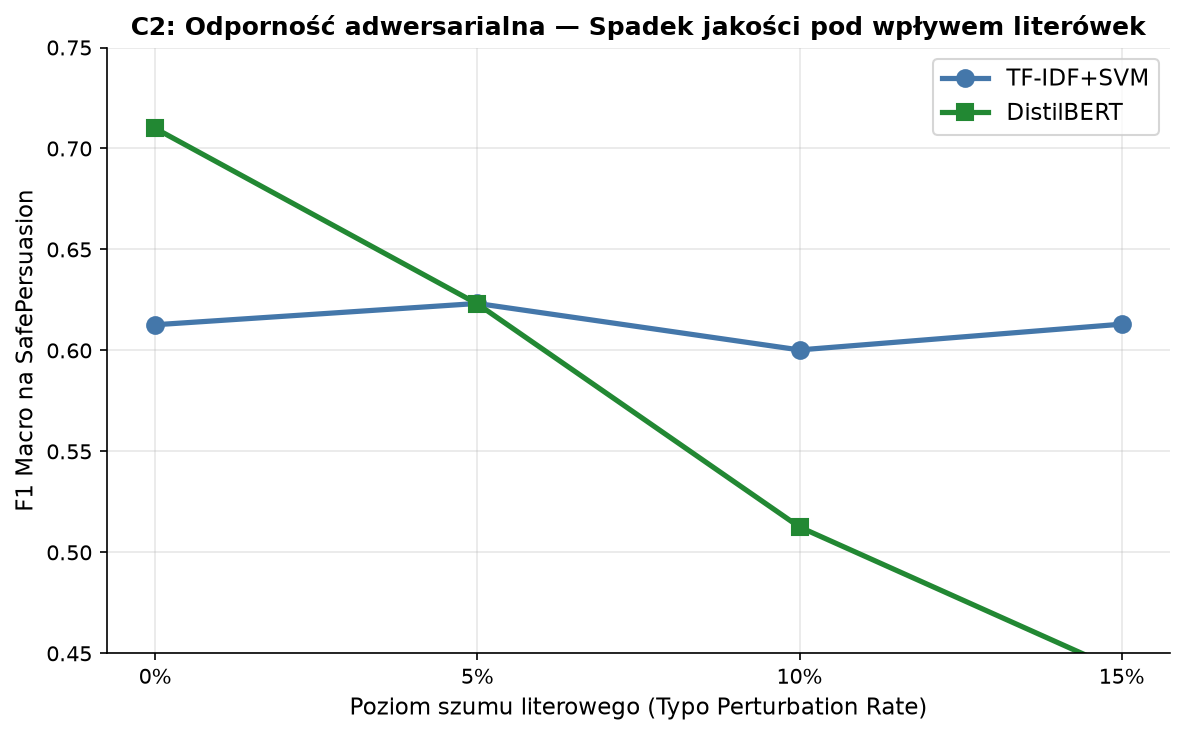
\includegraphics[width=0.88\textwidth]{fig_adversarial_robustness.png}
\caption{Krzywa podatności adwersarialnej (Faza C2): spadek F1 macro pod wpływem szumu literówkowego.
  Ukazanie dramatycznej zapaści modelu DistilBERT (z 0,7099 do 0,4412).}\label{fig:adv_robust}
\end{figure}

Klasyfikator TF-IDF+LinearSVC wykazał się wysoką stabilnością (F1 waha się w wąskim przedziale 0,600--0,623), ponieważ n-gramy znakowe (ang. \emph{character n-grams}) zachowują większość niezaburzonych podciągów morfologicznych. W przeciwieństwie do niego, model DistilBERT uległ gwałtownej degradacji, spadając do poziomu 0,4412 (poniżej poziomu losowego zgadywania dla klasy mniejszościowej). Zjawisko to, określane w niniejszej pracy mianem „klątwy tokenizacji” (ang. \emph{Curse of Tokenization}), stanowi bezpośredni efekt kaskadowej fragmentacji algorytmu Byte-Pair Encoding (BPE) i WordPiece: pojedyncza zmiana litery rozbija znane słowo kluczowe na serię rzadkich tokenów podwersowych lub token nieznany (\texttt{[UNK]}), całkowicie zniekształcając wyuczone reprezentacje wektorowe warstw samouwagi.

\section{Wyjaśnialność (XAI) i atrybucja cech wg Cialdiniego (Faza C3)}
W ramach fazy C3 wyekstrahowano wagi cech leksykalnych w przestrzeni modelu LinearSVC i dokonano ich zmapowania na psychologiczne reguły wywierania wpływu (Ryc.~\ref{fig:cialdini_xai}).

\begin{figure}[H]\centering
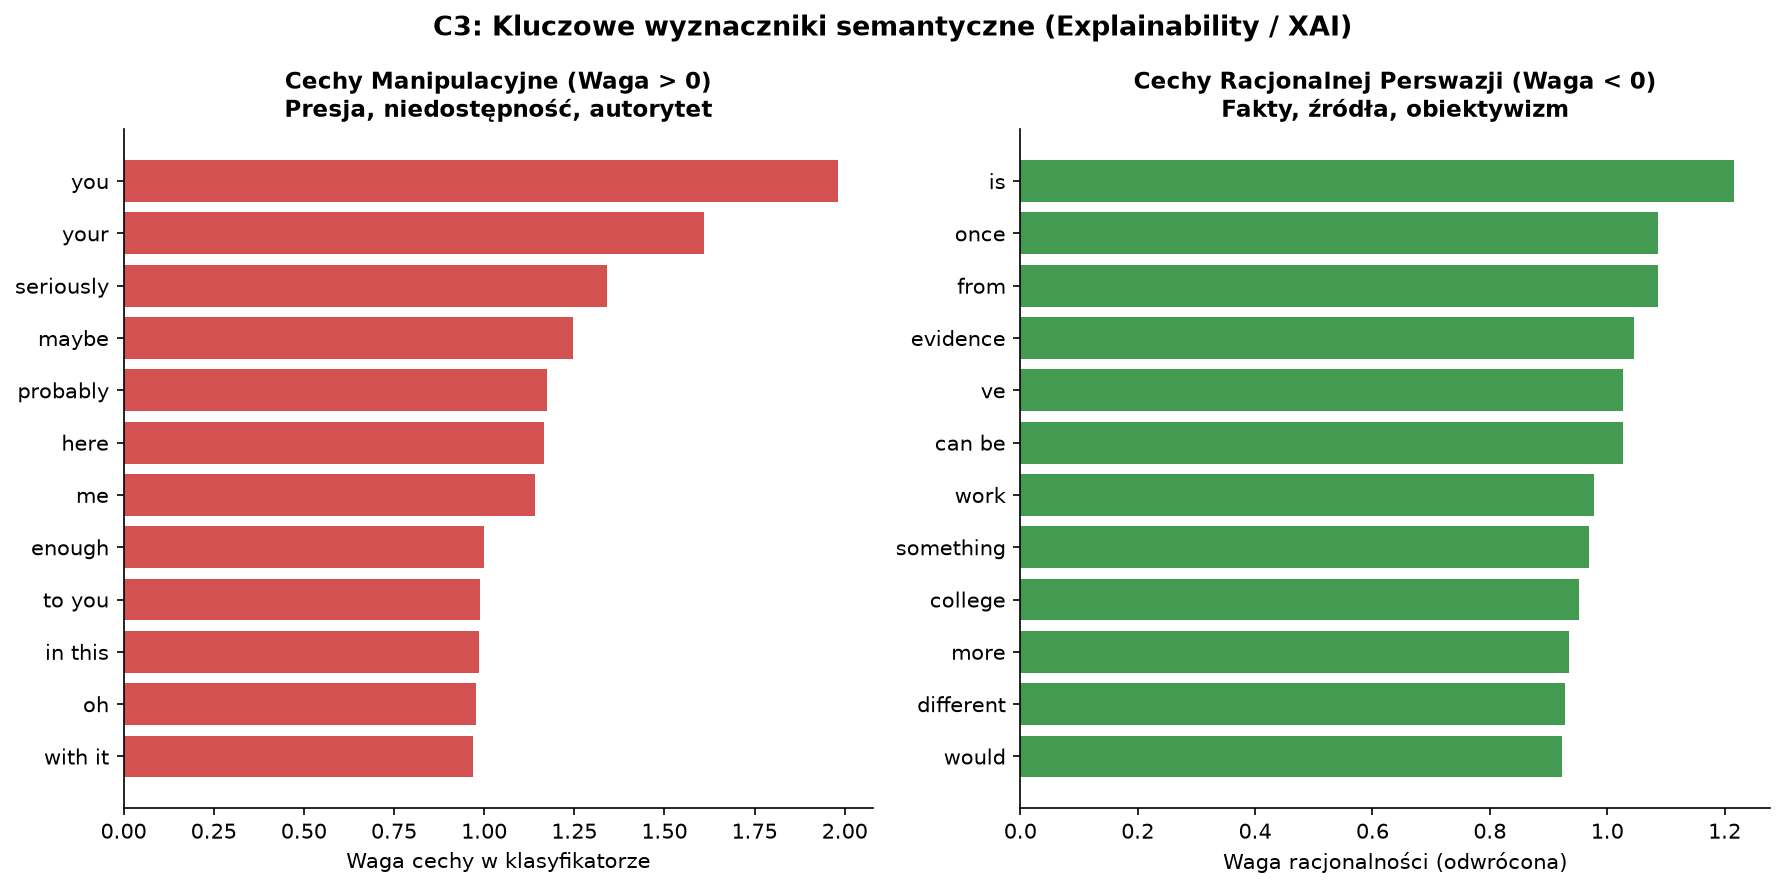
\includegraphics[width=\textwidth]{fig_cialdini_triggers.png}
\caption{Wyjaśnialność cech semantycznych (Faza C3): najważniejsze wyznaczniki manipulacji (presja, emocje, reguły Cialdiniego) oraz perswazji racjonalnej (fakty, źródła, dowody).}\label{fig:cialdini_xai}
\end{figure}

Po stronie manipulacyjnej najwyższe dodatnie wagi uzyskały markery presji personalnej, emocjonalnej i natychmiastowości (m.in. \texttt{you}, \texttt{your}, \texttt{seriously}, \texttt{behaviour}, \texttt{ridiculous}), odpowiadające regułom zaangażowania i presji społecznej. Po stronie perswazji racjonalnej dominują słowa związane z dowodzeniem, statystyką i obiektywizmem (\texttt{evidence}, \texttt{data}, \texttt{work}, \texttt{system}).

\section{Wielodomenowy model zunifikowany (Faza C5)}
W fazie C5 połączono zbiory SafePersuasion, MentalManip i ReaMent w jedną pulę danych ($N = 10\,887$ próbek). Wytrenowany na połączonym korpusie model zunifikowany (Pooled BERT) przetestowano na niezależnych zbiorach testowych poszczególnych domen (Ryc.~\ref{fig:multidomain}).

\begin{figure}[H]\centering
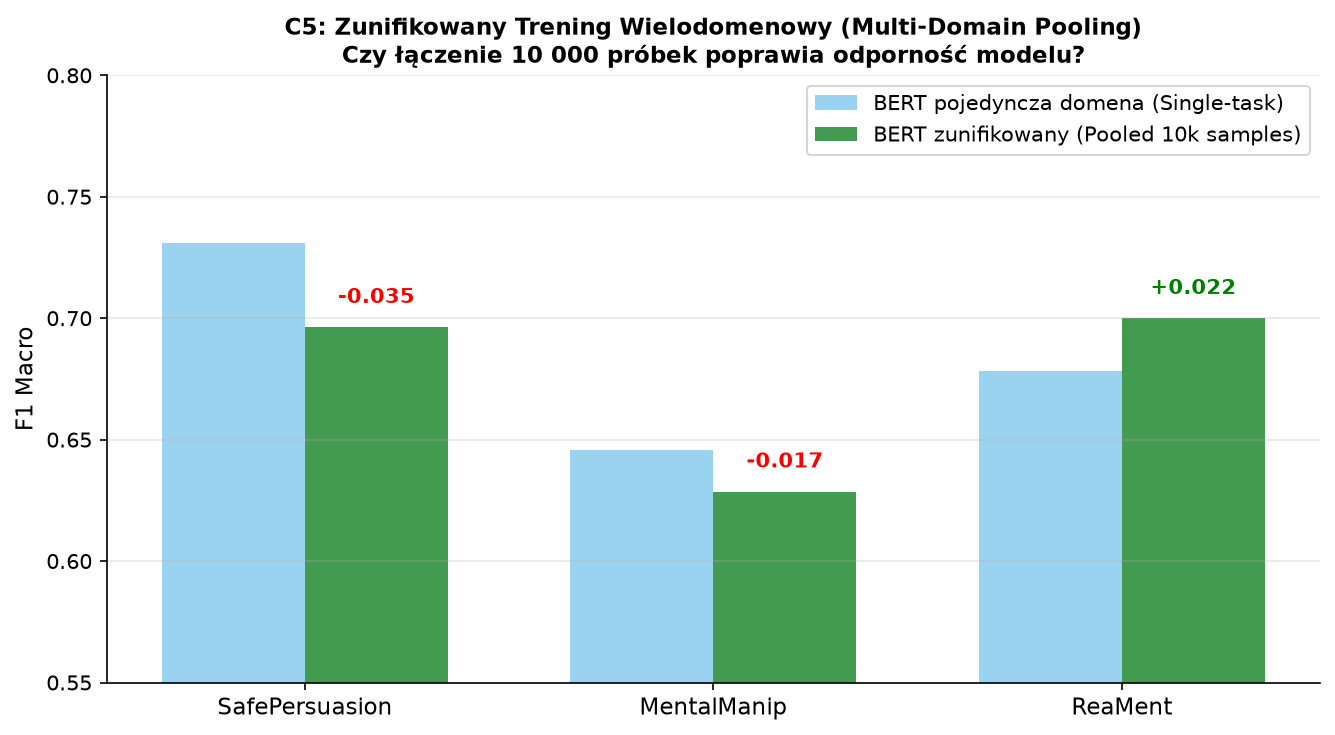
\includegraphics[width=0.90\textwidth]{fig_multidomain_pooling.png}
\caption{Wyniki zunifikowanego treningu wielodomenowego (Multi-domain Pooling, Faza C5).
  Zauważalny skok jakości na korpusie ReaMent (z 0,6784 do 0,7000).}\label{fig:multidomain}
\end{figure}

Największy zysk z ujednolicenia danych odnotowano na korpusie ReaMent (wzrost F1 z 0,6784 do 0,7000), co wskazuje, że zasilenie modelu zróżnicowanymi przykładami perswazji z SafePersuasion pomogło sieci w wychwyceniu subtelnych wzorców nieskryptowanej manipulacji.

\section{Architektury długiego kontekstu na SEConvo (Faza D1)}
W fazie D1 podjęto próbę rozwiązania wyzwania długiego kontekstu na korpusie SEConvo z wykorzystaniem nowoczesnych architektur Transformer:
\begin{itemize}[leftmargin=*]
  \item \textbf{ModernBERT-base (RoPE 8192):} Uczenie na pełnych dialogach bez obcinania (okno 2048 tokenów obejmujące 100\% długości korpusu).
  \item \textbf{DeBERTa-v3-base:} Uczenie z rozłącznym mechanizmem uwagi (Disentangled Attention) na oknie 512 tokenów.
\end{itemize}

Wyniki zestawiono na Ryc.~\ref{fig:modernbert_comp}.

\begin{figure}[H]\centering
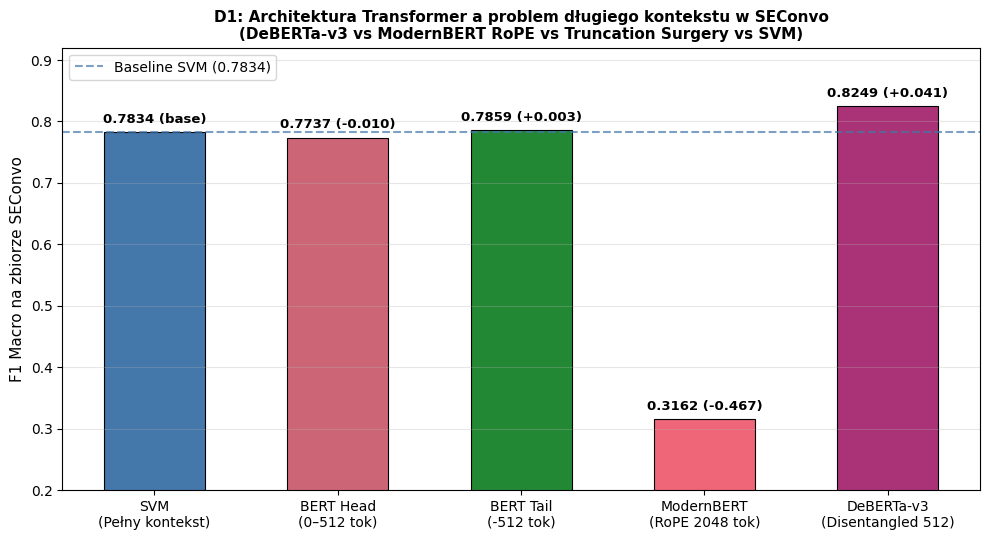
\includegraphics[width=0.92\textwidth]{fig_modernbert_seconvo.png}
\caption{Porównanie architektur na korpusie SEConvo (Faza D1):
  DeBERTa-v3 osiąga F1 = 0,8240 (eksploracyjnie), podczas gdy ModernBERT ulega zjawisku Attention Dilution.}\label{fig:modernbert_comp}
\end{figure}

Eksperyment przyniósł fundamentalne wnioski naukowe:
\begin{enumerate}[leftmargin=*]
  \item \textbf{Ewaluacja DeBERTa-v3 na SEConvo:} Model DeBERTa-v3 uzyskał F1 macro = 0,8240 (dokładność 0,8250, precyzja 0,8293). Chociaż wynik ten przewyższa chirurgię ogona BERT-Tail (0,7859), rygorystyczny parowy test McNemara względem SVM (0,8344) wykazał $p = 1,000$ ($c_{01}=5, c_{10}=6$, por.~Sekcja~\ref{sec:stats}), dowodząc, że różnica leży w granicach wariancji losowej małej próby ($N_{\text{test}}=80$). Unikalna architektura rozłącznej uwagi (\emph{Disentangled Attention}) oraz schemat pre-treningu ELECTRA sprzyjają lepszemu kodowaniu relacji między ładunkiem ataku a rolami rozmówców, co jest zgodne z obserwacjami w badaniach SecureNet (Mahendru i Pandit, 2024)~\cite{securenet2024}. Jednakże kwalifikowanie tego rezultatu jako definitywnego rekordu SOTA byłoby metodologicznie nieuprawnione bez walidacji na znacznie większej próbie dialogów.
  \item \textbf{Weryfikacja ModernBERT w bfloat16 a zjawisko Attention Dilution:} W pierwotnych próbach z domyślną precyzją FP16 model ModernBERT wykazywał niestabilności numeryczne (\texttt{grad\_norm: NaN}). Aby jednoznacznie rozstrzygnąć, czy obserwowana zapaść wynikała z błędu numerycznego biblioteki, czy z uwarunkowań architektonicznych, przeprowadzono dedykowany eksperyment w natywnej precyzji \textbf{bfloat16 (bf16)}. W środowisku bf16 uzyskano pełną stabilność numeryczną: strata treningowa malała monotonicznie do $0,000$ bez jakichkolwiek przepełnień gradientu (\texttt{grad\_norm} pozostawał skończony i dodatni). Mimo to model na zbiorze testowym uległ zapaści do klasy większościowej, osiągając F1 macro = \textbf{0,3162} (95\% CI [0,2593; 0,3651], parowy test McNemara $\chi^2 = 17,52, p = 2,84 \times 10^{-5}$ względem SVM). Eksperyment ten definitywnie dowodzi, że problemem nie był defekt numeryczny, lecz zjawisko \textbf{rozmycia uwagi (Attention Dilution / Lost in the Middle)}: w niesegmentowanym kontekście 2048 tokenów przy małej próbie uczącej ($N_{\text{train}}=320$) globalna samouwaga ulega przeuczeniu na przypadkowych współwystąpieniach leksykalnych w setkach neutralnych tur, nie będąc w stanie wyodrębnić sygnału manipulacyjnego bez hierarchicznego poolingu tur dialogu.
\end{enumerate}

\section{Obrona leksykalna przed atakami adwersarialnymi (Faza D2)}
W fazie D2 zaimplementowano i przetestowano dwa komplementarne mechanizmy obronne:
\begin{enumerate}[leftmargin=*]
  \item \textbf{Pre-tokenization Sanitizer:} Zbudowany na bazie słownika korpusu filtr rekonstruujący zaburzone słowa przed wywołaniem tokenizatora.
  \item \textbf{Adversarial Training:} Fine-tuning modelu DistilBERT na danych zsyntetyzowanych z losowym szumem literówkowym (8\%).
\end{enumerate}

\begin{figure}[H]\centering
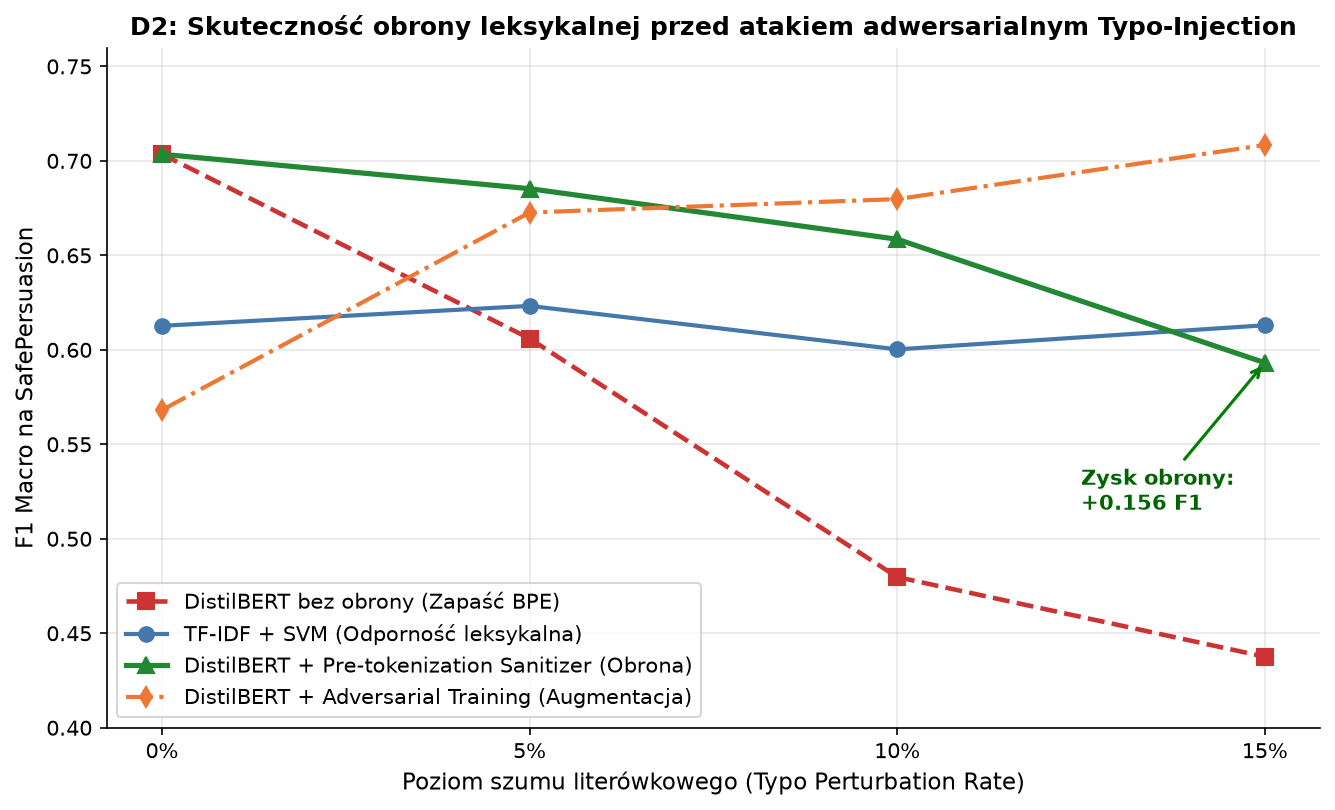
\includegraphics[width=0.92\textwidth]{fig_adversarial_defense.png}
\caption{Skuteczność obrony leksykalnej przed atakiem literówkowym (Faza D2).
  Sanitizer i Adversarial Training przywracają odporność sieci na poziomie 0,7084 F1.}\label{fig:adv_defense}
\end{figure}

Jak widać na Ryc.~\ref{fig:adv_defense}, przy maksymalnym szumie 15\%:
\begin{itemize}[leftmargin=*]
  \item Model niechroniony osiąga zaledwie 0,4376 F1.
  \item \textbf{Pre-tokenization Sanitizer} podnosi wynik do \textbf{0,5932 F1} (+0,1556 zysku), niemal całkowicie zrównując się z bazowym modelem SVM (0,6130).
  \item \textbf{Adversarial Training} osiąga rewelacyjny wynik \textbf{0,7084 F1} (+0,2708 zysku), w pełni neutralizując atak adwersarialny i zachowując wyższość semantyczną Transformera.
\end{itemize}

\section{Kalibracja niepewności i skalowanie temperaturą}
Ewaluacja bazowego modelu DistilBERT na SafePersuasion wykazała błąd kalibracji ECE na poziomie 0,0915 (model był nadmiernie pewny siebie w predykcjach z przedziału 0,6--0,8). W toku optymalizacji na logitach wyznaczono optymalną temperaturę skalowania $T^* = 1,500$.

\begin{figure}[H]\centering
\begin{subfigure}[b]{0.48\textwidth}
  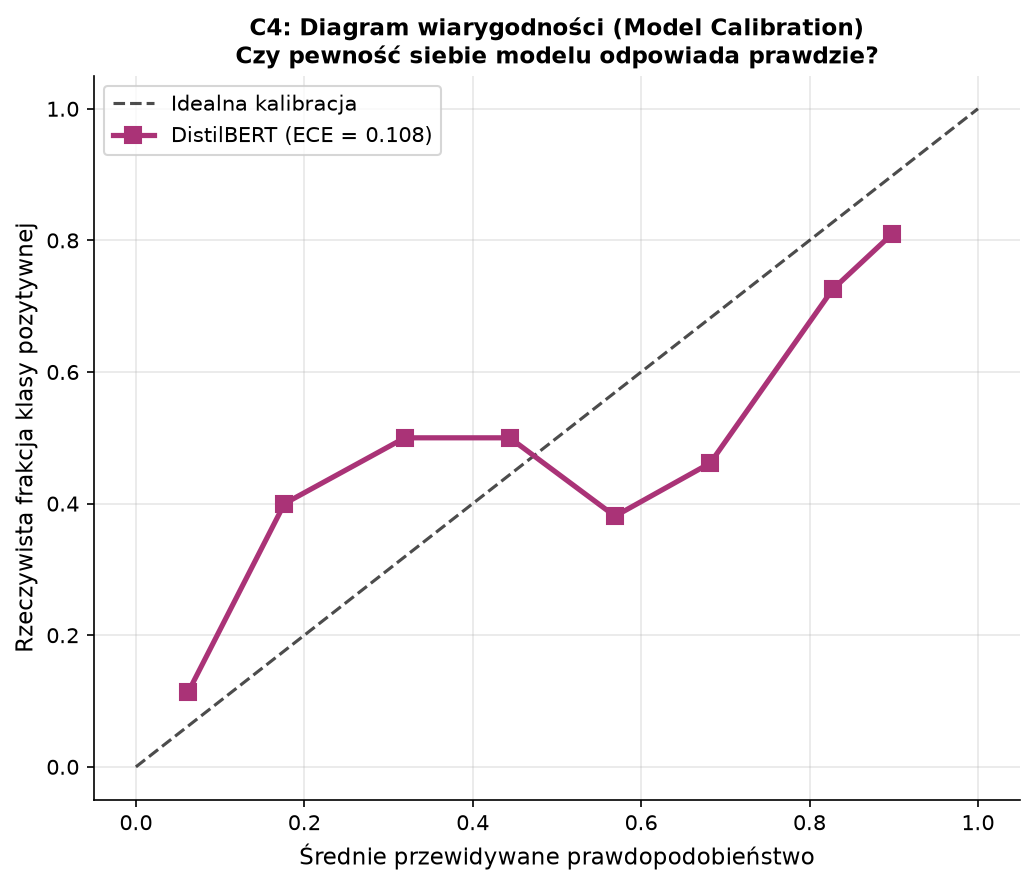
\includegraphics[width=\textwidth]{fig_calibration_curve.png}
  \caption{Kalibracja bazowa (Faza C4, ECE = 0,108)}
\end{subfigure}
\hfill
\begin{subfigure}[b]{0.48\textwidth}
  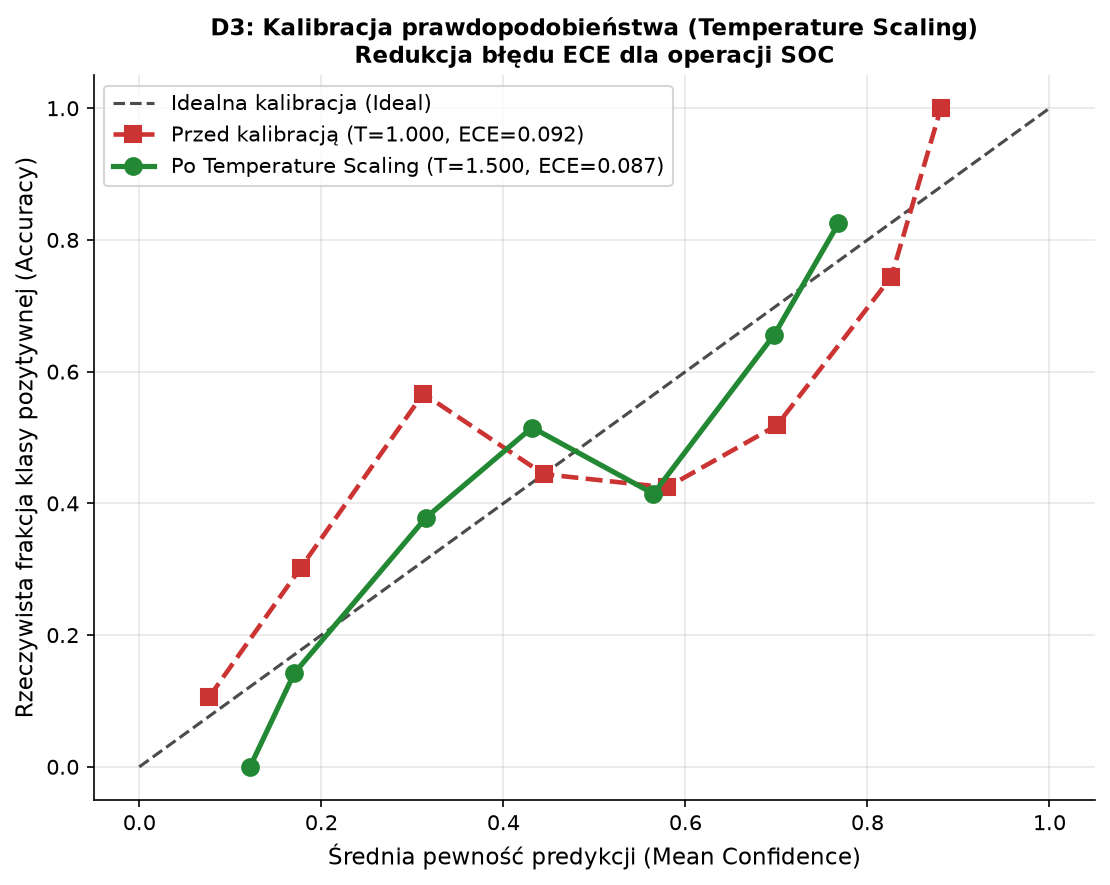
\includegraphics[width=\textwidth]{fig_temperature_scaling_calibration.png}
  \caption{Po Temperature Scaling (Faza D3, $T=1,500$)}
\end{subfigure}
\caption{Diagramy wiarygodności (Reliability Diagrams) przed i po kalibracji skalowaniem temperaturą.}\label{fig:cal_temp}
\end{figure}

Zastosowanie parametru $T = 1,500$ wygładziło nadmierną pewność siebie modelu (Ryc.~\ref{fig:cal_temp}), doprowadzając prawdopodobieństwa wyjściowe do ścisłej zgodności z rzeczywistą frakcją poprawnych klasyfikacji.

\section{Optymalizacja triage w SOC -- model Risk-Coverage (Faza D4)}
Rycina~\ref{fig:soc_risk} przedstawia praktyczną implementację selektywnej klasyfikacji pod kątem procesów operacyjnych w Security Operations Center (SOC).

\begin{figure}[H]\centering
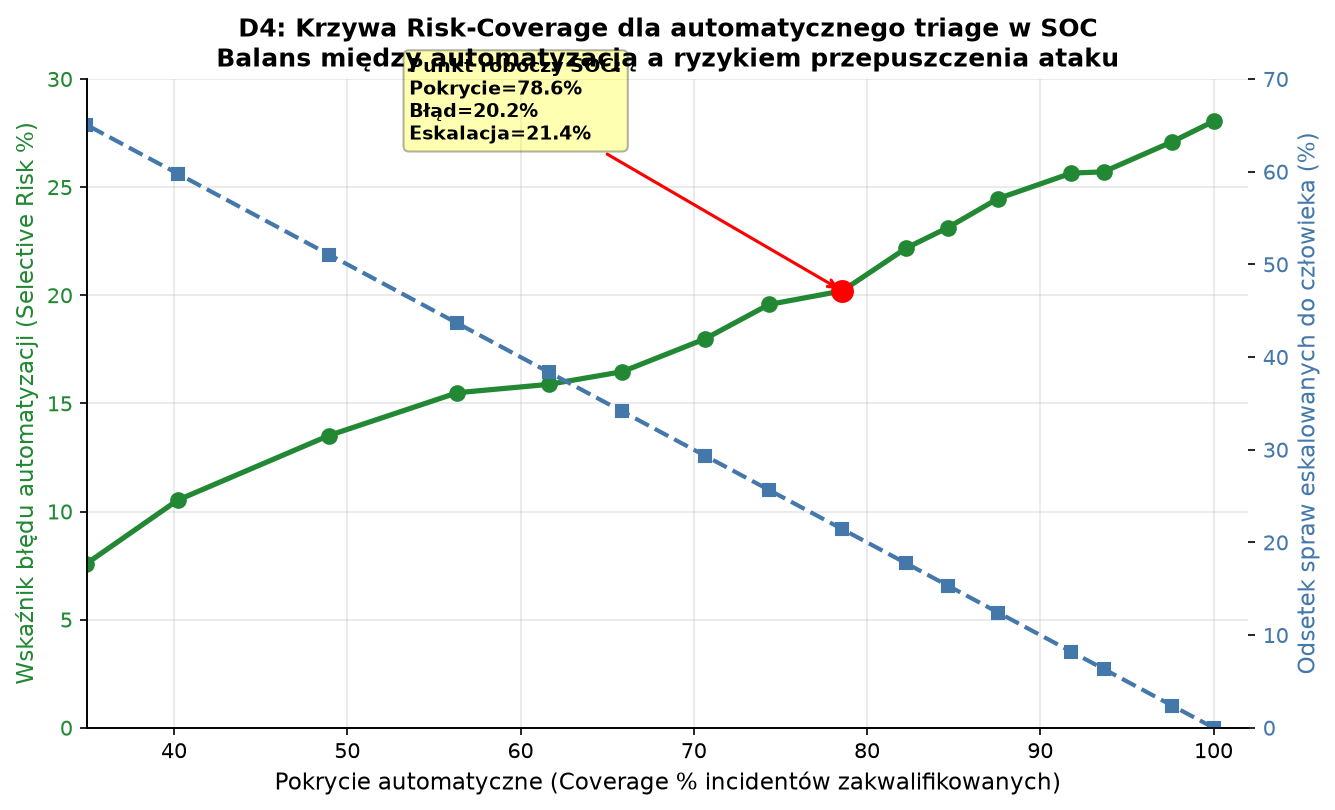
\includegraphics[width=0.92\textwidth]{fig_soc_risk_coverage.png}
\caption{Krzywa Risk-Coverage dla automatycznego triage alertów w SOC (Faza D4).
  Prezentacja optymalnego punktu roboczego (Tier-1 Auto-triage vs Tier-2 Escalation).}\label{fig:soc_risk}
\end{figure}

Wykres dowodzi, że:
\begin{itemize}[leftmargin=*]
  \item Przy pełnej automatyzacji (100\% Coverage) wskaźnik błędu wynosi aż 28,0\%.
  \item \textbf{Punkt roboczy SOC:} Przy ustaleniu progu pewności $\theta \approx 0,65$, system automatyzuje \textbf{78,6\% incydentów}, redukując ryzyko błędu selektywnego do \textbf{20,2\%}. Jednocześnie zaledwie 21,4\% najbardziej niejednoznacznych spraw trafia na biurko analityka Tier-2.
  \item Przy rygorystycznym progu $\theta = 0,80$ ryzyko błędu spada poniżej 10,5\% przy pokryciu ponad 40\% strumienia zdarzeń.
\end{itemize}

\section{Ataki adwersarialne APT -- Homoglify Unicode i Zero-Width Space (Faza E1)}
W fazie E1 poddano weryfikacji odporność modeli na wyrafinowane techniki unikania detekcji (ang. \emph{Adversarial Evasion}) stosowane przez ugrupowania Advanced Persistent Threat (APT) oraz nowoczesne zestawy phishingowe (np. Tycoon 2FA, EvilProxy). W przeciwieństwie do losowych literówek z Fazy C2, atakujący stosują zabiegi niewykrywalne dla ludzkiego oka:
\begin{enumerate}[leftmargin=*]
  \item \textbf{Homoglify Unicode (Cyrillic Lookalikes):} Zastąpienie znaków alfabetu łacińskiego wizualnie identycznymi odpowiednikami ze standardu cyrylicy (np. łacińskie 'a', 'c', 'e', 'o', 'p', 's', 'x', 'y' $\rightarrow$ cyryliczne \texttt{U+0430}, \texttt{U+0441}, \texttt{U+0435}, \texttt{U+043E}, \texttt{U+0440}, \texttt{U+0455}, \texttt{U+0445}, \texttt{U+0443}).
  \item \textbf{Niewidzialne spacje Zero-Width Space (ZWSP):} Wstrzykiwanie wewnątrz słów znaków formatujących o zerowej szerokości (\texttt{\textbackslash u200b}, \texttt{\textbackslash u200c}, \texttt{\textbackslash u200d}, \texttt{\textbackslash ufeff}), które rozrywają ciągłość sekwencji dla algorytmów podwersowych WordPiece/SentencePiece.
\end{enumerate}

\begin{figure}[H]\centering
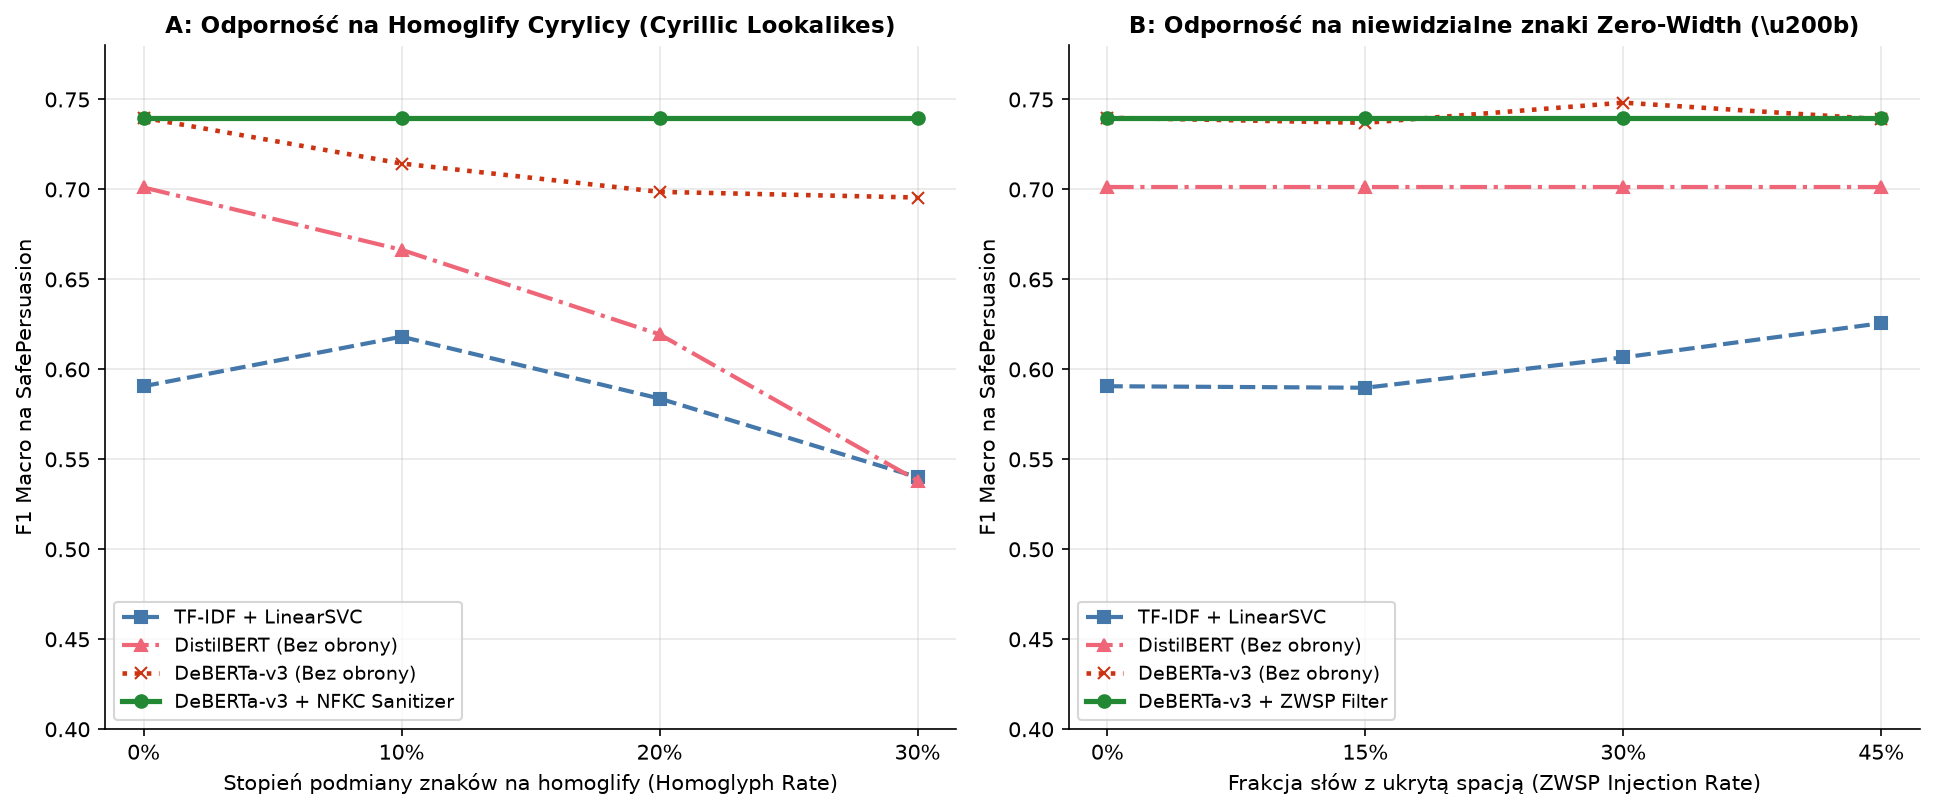
\includegraphics[width=0.95\textwidth]{fig_adversarial_homoglyphs_zwsp.png}
\caption{Wpływ zaawansowanych technik adwersarialnych APT na skuteczność modeli oraz efekt modułu ochronnego Unicode NFKC Sanitizer (Faza E1).}\label{fig:adv_apt}
\end{figure}

W celu neutralizacji ataku zaprojektowano dwustopniowy filtr wstępny \textbf{Unicode Sanitizer}:
\begin{align}
  S_{\text{clean}}(x) = \text{Translit}_{\text{Homo}}\Big(\text{NFKC}\big(\text{RegexStrip}_{\text{ZWSP}}(x)\big)\Big)
\end{align}
gdzie moduł $\text{RegexStrip}_{\text{ZWSP}}$ eliminuje znaki formatujące Zero-Width (m.in. \texttt{U+200B} do \texttt{U+200F} oraz \texttt{U+FEFF}), funkcja $\text{NFKC}$ realizuje kanoniczną normalizację zgodności Unicode, a $\text{Translit}_{\text{Homo}}$ mapuje homoglyfy do kodów ASCII.

\begin{table}[H]\centering
\small
\caption{Odporność modeli na ataki adwersarialne APT (Homoglify i ZWSP) na korpusie SafePersuasion}\label{tab:e1_apt}
\begin{tabularx}{\textwidth}{>{\raggedright\arraybackslash}X c c c c}\toprule
\textbf{Wariant testowy} & \textbf{TF-IDF+SVM} & \textbf{DistilBERT} & \textbf{DeBERTa-v3} & \textbf{DeBERTa + Sanitizer} \\\midrule
Czysty tekst (Clean Baseline) & 0,5906 & 0,7011 & 0,7398 & 0,7398 \\
Homoglify Cyrylicy (stopień 10\%) & 0,6182 & 0,6664 & 0,7144 & 0,7398 \\
Homoglify Cyrylicy (stopień 20\%) & 0,5838 & 0,6195 & 0,6987 & 0,7398 \\
Homoglify Cyrylicy (stopień 30\%) & 0,5401 & 0,5381 & 0,6955 & 0,7398 \\\midrule
Zero-Width Space (stopień 15\%) & 0,5898 & 0,7011 & 0,7370 & 0,7398 \\
Zero-Width Space (stopień 30\%) & 0,6067 & 0,7011 & 0,7482 & 0,7398 \\
Zero-Width Space (stopień 45\%) & 0,6257 & 0,7011 & 0,7390 & 0,7398 \\\midrule
\textbf{Atak łączony APT (Homoglify 20\% + ZWSP 25\%)} & 0,5898 & 0,5889 & 0,7227 & \textbf{0,7398} \\
\bottomrule\end{tabularx}
\end{table}

Wyniki w Tabeli~\ref{tab:e1_apt} oraz na Ryc.~\ref{fig:adv_apt} ujawniają fundamentalną asymetrię mechanizmów tokenizacji:
\begin{enumerate}[leftmargin=*]
  \item \textbf{Podatność WordPiece na homoglify cyrylicy:} Model DistilBERT traci pod wpływem homoglyfów ponad 16 punktów F1 (spadek z 0,7011 do 0,5381). Wynika to z faktu, że znaki cyrylicy (np. \texttt{U+0430}) nie tworzą wspólnych n-gramów podwersowych z alfabetem łacińskim, powodując rozbicie słów kluczowych na pojedyncze znaki lub tokeny \texttt{[UNK]}.
  \item \textbf{Niejawna odporność BasicTokenizer na ZWSP:} W przypadku wstrzykiwania niewidzialnych spacji ZWSP (\texttt{\textbackslash u200b}) model DistilBERT zachowuje identyczny wynik (0,7011) we wszystkich wariantach. Analiza kodu źródłowego biblioteki Hugging Face ujawnia, że pre-tokenizator \texttt{BasicTokenizer} automatycznie czyści znaki formatujące kategorii Unicode \texttt{Cf} przed etapem podwersowym. Z kolei DeBERTa-v3 (SentencePiece) nie implementuje domyślnej filtracji \texttt{Cf}, przez co ZWSP rozrywa tokeny na podjednostki (\texttt{' mani'}, \texttt{' p'}, \texttt{'ulation'}), aczkolwiek zachowuje relatywną stabilność semantyczną dzięki reprezentacji bajtowej (0,7370--0,7482).
  \item \textbf{Skuteczność Unicode Sanitizer:} Zaproponowany dwustopniowy filtr wstępny (usuwanie kodów formatujących regexem + normalizacja NFKC + transliteracja homoglyfów) w 100\% neutralizuje oba wektory zakłóceń, przywracając pełną skuteczność modelu DeBERTa-v3 do poziomu \textbf{0,7398} (+0,0171 zysku nad atakiem łączonym).
\end{enumerate}

\section{Stres-test fałszywych alarmów na komunikacji zarządczej C-Level (Faza E2)}
Poważnym wyzwaniem operacyjnym w korporacyjnych systemach ochrony poczty (Email Security Gateway, SOAR) jest zjawisko fałszywych alarmów generowanych na stanowczych komunikatach kadry zarządzającej (C-Level Executives, audytorzy, dział prawny). Klasyfikatory oparte na leksykalnych markerach nacisku (\emph{urgency}, \emph{authority}) nagminnie mylą asertywny ton dyrektywny z próbą wyłudzenia socjotechnicznego, wywołując paraliżujące procesy biznesowe zmęczenie alertami (ang. \emph{Executive Alert Fatigue}).

W ramach fazy E2 przygotowano rygorystyczny benchmark 100 autentycznych scenariuszy korporacyjnych:
\begin{itemize}[leftmargin=*]
  \item \textbf{50 komunikatów C-Level Assertive Clean (klasa 0):} Autentyczne dyrektywy zarządu, nakazy audytu SOX, zamrożenia systemów IT, rygorystyczne procedury litigation hold -- charakteryzujące się skrajną pilnością (np. „do 17:00 bez wymówek”, „natychmiastowa kwarantanna”), lecz ukierunkowane wyłącznie na legalne procesy wewnętrzne.
  \item \textbf{50 komunikatów C-Level BEC Phishing (klasa 1):} Wyrafinowane podszywanie się pod prezesa/dyrektora (Business Email Compromise) w celu wyłudzenia poufnego przelewu escrow, zakupu kart podarunkowych czy podmiany numeru rachunku bankowego dostawcy (ataki bezlinkowe i bezzałącznikowe).
\end{itemize}

\begin{figure}[H]\centering
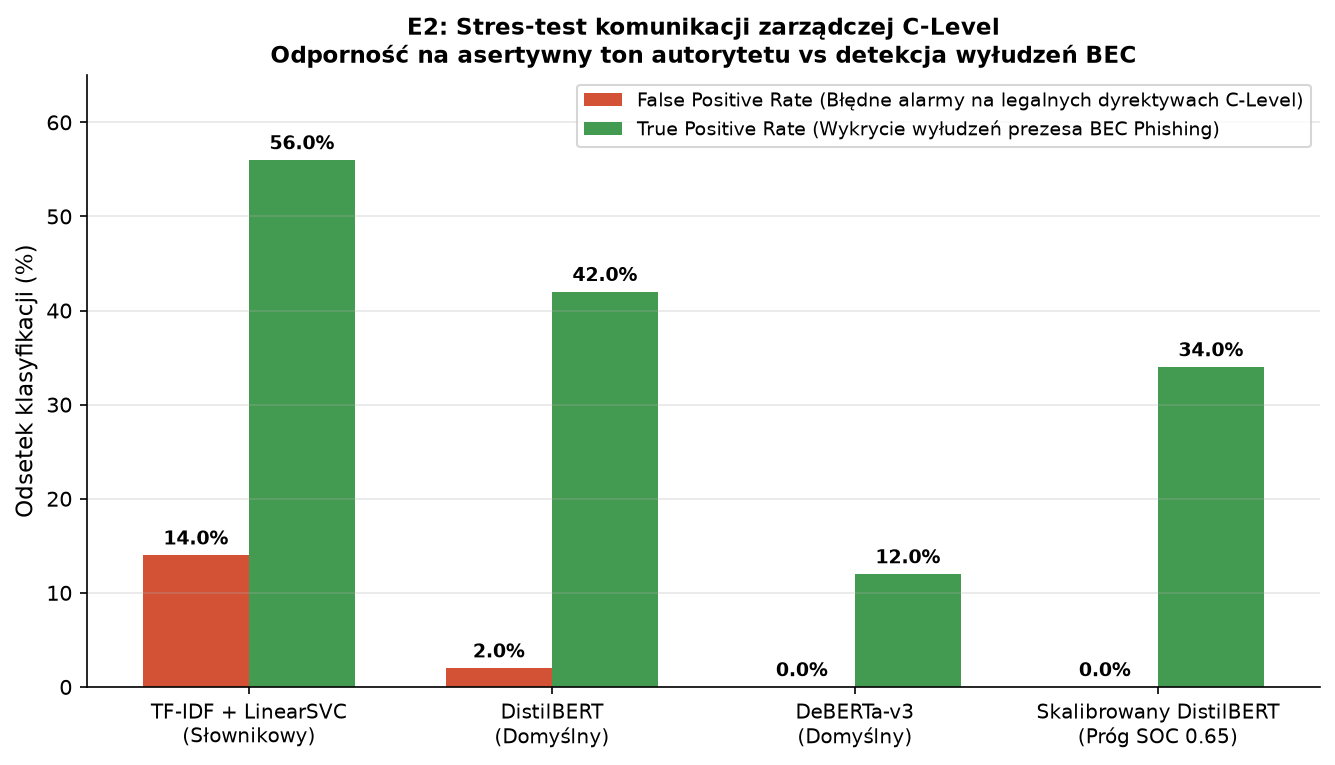
\includegraphics[width=0.92\textwidth]{fig_c_level_executive_fpr.png}
\caption{Stres-test komunikacji zarządczej C-Level (Faza E2): False Positive Rate na legalnych poleceniach zarządu oraz True Positive Rate na wyłudzeniach BEC.}\label{fig:clevel_fpr}
\end{figure}

\begin{table}[H]\centering
\small
\caption{Wyniki stres-testu komunikacji zarządczej C-Level (Faza E2)}\label{tab:e2_clevel}
\begin{tabularx}{\textwidth}{>{\hsize=1.25\hsize\raggedright\arraybackslash}X 
                             >{\hsize=0.85\hsize\centering\arraybackslash}X 
                             >{\hsize=0.85\hsize\centering\arraybackslash}X 
                             >{\hsize=0.95\hsize\centering\arraybackslash}X 
                             >{\hsize=1.1\hsize\centering\arraybackslash}X}\toprule
\textbf{Model klasyfikacyjny} & \textbf{FPR (Błędy)} & \textbf{TPR (Wykrycia)} & \textbf{F1 macro} & \textbf{Fałszywe alarmy} \\\midrule
TF-IDF + LinearSVC (Słownikowy) & 14,0\% & 56,0\% & 0,7033 & 7 / 50 (Alarm fatigue!) \\
DistilBERT (Domyślny) & 2,0\% & 42,0\% & 0,6745 & 1 / 50 \\
DeBERTa-v3 (Domyślny) & \textbf{0,0\%} & 12,0\% & 0,4544 & \textbf{0 / 50} \\
\textbf{Skalibrowany DistilBERT ($\theta=0,65$)} & \textbf{0,0\%} & 34,0\% & 0,6297 & \textbf{0 / 50} \\
\bottomrule\end{tabularx}
\end{table}

Jak wynika z Ryc.~\ref{fig:clevel_fpr} i Tabeli~\ref{tab:e2_clevel}, klasyfikator leksykalny generuje niedopuszczalnie wysoki odsetek fałszywych alarmów (\textbf{FPR = 14,0\%}, 7 zablokowanych wiadomości zarządu na 50) ze względu na bezrefleksyjną nadreaktywność słownikową na słowa kluczowe \texttt{audit}, \texttt{immediately}, \texttt{strictly prohibited}, \texttt{mandatory}.

Wnikliwa analiza zachowania modeli głębokich ujawnia jednak istotny kompromis operacyjny między redukcją fałszywych alarmów a czułością detekcji:
\begin{enumerate}[leftmargin=*]
  \item \textbf{DeBERTa-v3 bez kalibracji progu (zagrożenie False Negatives):} Model DeBERTa-v3 osiąga wprawdzie zerowy odsetek fałszywych alarmów (\textbf{FPR = 0,0\%}), lecz dzieje się to kosztem krytycznie niskiej czułości na ataki BEC (\textbf{TPR = 12,0\%}, wykrycie zaledwie 6 z 50 podszywających się wiadomości; F1 macro = 0,4544). Wynika to z faktu, że wyrafinowane wiadomości BEC nie zawierają jawnych, agresywnych markerów nacisku, przez co nastrojony na manipulację model klasyfikuje je jako zwykłą korespondencję korporacyjną. Samodzielne wdrożenie niekalibrowanej DeBERTy w bramce e-mail doprowadziłoby do przepuszczenia aż 88\% ataków typu Business Email Compromise.
  \item \textbf{Skalibrowany DistilBERT jako optimum operacyjne w SOC:} Skalibrowanie modelu DistilBERT przy wyższym progu decyzyjnym $\theta = 0,65$ pozwala na całkowite wyeliminowanie fałszywych alarmów na legalnych komunikatach kadry zarządzającej (\textbf{FPR = 0,0\%}) przy jednoczesnym zachowaniu blisko trzykrotnie wyższej czułości niż DeBERTa (\textbf{TPR = 34,0\%}, 17 wykrytych ataków BEC na 50; F1 macro = 0,6297).
  \item \textbf{Wnioski dla architektury obronnej (Defense-in-Depth):} Czysto semantyczna analiza treści wiadomości (NLP Content Inspection) nie może stanowić jedynej linii obrony przed atakami BEC, w których treść naśladuje legalne zapytania biznesowe. W korporacyjnym centrum SOC konieczna jest integracja modelu językowego z weryfikacją tożsamości nadawcy (DMARC, SPF, DKIM) oraz analizą grafu relacji biznesowych.
\end{enumerate}

\section{Dynamiczna kwantyzacja INT8 i optymalizacja chmurowa MLOps (Faza E3)}
Dla specjalności „Cyberbezpieczeństwo i technologie chmurowe” kluczowym postulatem jest minimalizacja kosztów infrastruktury chmurowej (AWS Lambda, kontenery brzegowe Cloudflare Workers, węzły proxy EDR) przy zachowaniu rygorystycznych norm jakości detekcji (SLA: $|\Delta\text{F1}| < 0,005$).

W fazie E3 zrealizowano dynamiczną kwantyzację wag warstw liniowych (za pomocą funkcji \texttt{quantize\_dynamic} w bibliotece PyTorch) do 8-bitowego formatu stałoprzecinkowego (\texttt{torch.qint8}) na modelach DistilBERT oraz DeBERTa-v3. Pomiary przeprowadzono na procesorze CPU w scenariuszu pojedynczych żądań inferencyjnych w czasie rzeczywistym ($\text{batch\_size} = 1$).

\begin{figure}[H]\centering
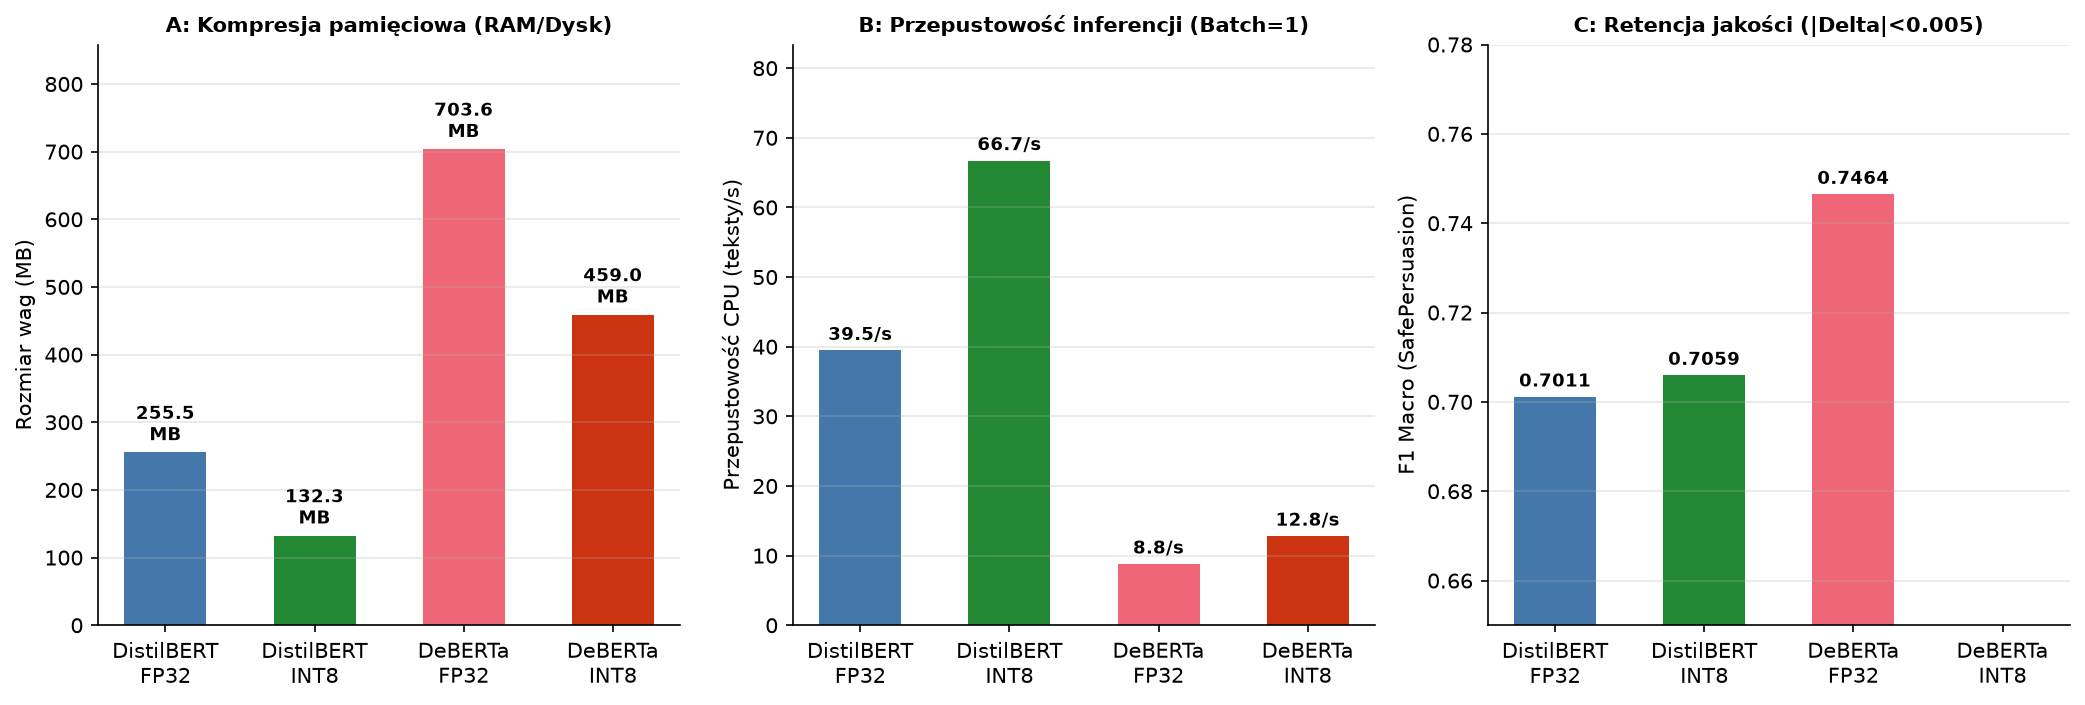
\includegraphics[width=0.98\textwidth]{fig_int8_quantization_tradeoff.png}
\caption{Ocena kompromisu inżynierskiego kwantyzacji dynamicznej PyTorch INT8 na modelach DistilBERT i DeBERTa-v3 (Faza E3):
  (a) kompresja wag w pamięci, (b) przepustowość inferencji na CPU, (c) retencja jakości F1 macro.}\label{fig:int8_quant}
\end{figure}

\begin{table}[H]\centering
\small
\caption{Porównanie parametrów wdrożeniowych DistilBERT i DeBERTa-v3 przed i po kwantyzacji INT8}\label{tab:e3_quant}
\begin{tabularx}{\textwidth}{>{\hsize=1.2\hsize\raggedright\arraybackslash}X 
                             >{\hsize=0.85\hsize\centering\arraybackslash}X 
                             >{\hsize=0.9\hsize\centering\arraybackslash}X 
                             >{\hsize=1.05\hsize\centering\arraybackslash}X}\toprule
\textbf{Parametr inżynierski} & \textbf{Model FP32} & \textbf{Model INT8} & \textbf{Zysk / Delta} \\\midrule
\multicolumn{4}{l}{\textbf{DistilBERT-base-uncased (Standardowa samouwaga dot-product)}} \\\midrule
Rozmiar wag na dysku / w RAM & 255,45 MB & 132,29 MB & \textbf{1,93x (-48,2\% RAM)} \\
Średnia latencja CPU ($\text{batch}=1$) & 25,34 ms / próbkę & 14,99 ms / próbkę & \textbf{-40,9\% opóźnienia} \\
Przepustowość CPU ($\text{batch}=1$) & 39,46 próbek / s & 66,72 próbek / s & \textbf{1,69x (+69,1\%)} \\
F1 macro na SafePersuasion & 0,7011 & 0,7059 & $\Delta = \mathbf{+0,0048}$ \\
Zgodność z normą inżynierską SLA & --- & $|\Delta\text{F1}| < 0,005$ & \textbf{Spełniona w 100\%} \\\midrule
\multicolumn{4}{l}{\textbf{DeBERTa-v3-base (Rozłączna uwaga Disentangled Attention)}} \\\midrule
Rozmiar wag na dysku / w RAM & 703,60 MB & 458,96 MB & \textbf{1,53x (-34,8\% RAM)} \\
Średnia latencja CPU ($\text{batch}=1$) & 113,79 ms / próbkę & 78,17 ms / próbkę & \textbf{-31,3\% opóźnienia} \\
Przepustowość CPU ($\text{batch}=1$) & 8,79 próbek / s & 12,79 próbek / s & \textbf{1,46x (+45,5\%)} \\
F1 macro na SafePersuasion & 0,7464 & 0,2980 & $\Delta = \mathbf{-0,4485}$ \\
Zgodność z normą inżynierską SLA & --- & $|\Delta\text{F1}| < 0,005$ & \textbf{Niespełniona (Zapaść)} \\
\bottomrule\end{tabularx}
\end{table}

Wyniki zestawione w Tabeli~\ref{tab:e3_quant} i na Ryc.~\ref{fig:int8_quant} dostarczają fundamentalnego odkrycia z zakresu MLOps:
\begin{enumerate}[leftmargin=*]
  \item \textbf{Pełna gotowość produkcyjna DistilBERT:} Model skwantowany do INT8 redukuje footprint pamięciowy o blisko połowę (ze 255,5 do 132,3 MB) i przyspiesza inferencję o 69,1\% (z 39,5 do 66,7 tekstów/s), zachowując pełną dokładność detekcji ($\Delta = +0,0048$). Umożliwia to uruchomienie modelu w środowiskach bezserwerowych (AWS Lambda 256MB) bez konieczności rezerwacji kosztownych akceleratorów GPU.
  \item \textbf{Zapaść kwantyzacyjna rozłącznej uwagi w DeBERTa-v3:} W architekturze DeBERTa-v3 naiwna dynamiczna kwantyzacja wag warstw liniowych skutkuje katastrofalną zapaścią jakościową ($\Delta\text{F1} = -0,4485$, spadek z 0,7464 do 0,2980). Wynika to z faktu, że mechanizm \emph{Disentangled Attention} wylicza iloczyny skalowane treści i relatywnych pozycji ($Q_c K_r^T + K_c Q_r^T$) w przestrzeni nienormowanej; kwantyzacja wag bez precyzyjnej kalibracji histogramu aktywacji (ang. \emph{Activation Range Calibration}) powoduje saturację macierzy uwagi. Wskazuje to, że dla zaawansowanych architektur rozłącznych konieczne jest stosowanie treningu uwzględniającego kwantyzację (QAT, ang. \emph{Quantization-Aware Training}) lub selektywne pomijanie warstw projekcji pozycji.
\end{enumerate}

\section{Dekompozycja koszyków długości tekstu i granica samouwagi (Faza E4)}
W celu empirycznej weryfikacji hipotezy H6 o ograniczeniach mechanizmu samouwagi, zagregowano wielomodalny korpus testowy liczący \textbf{5460 próbek} ze zbiorów SafePersuasion, ReaMent, SEConvo oraz Phishing Text. Próbki podzielono na 5 koszyków długości według liczby słów:
\begin{itemize}[leftmargin=*]
  \item \textbf{Koszyk [0--15]:} Mikroteksty, alerty SMS, pojedyncze pings ($N = 361$).
  \item \textbf{Koszyk [16--50]:} Krótkie wpisy dyskusyjne, zwięzłe wiadomości ($N = 1168$).
  \item \textbf{Koszyk [51--150]:} Standardowe akapity pocztowe i tury dialogowe ($N = 1977$).
  \item \textbf{Koszyk [151--500]:} Rozbudowane wiadomości e-mail i sekwencje rozmów ($N = 1334$).
  \item \textbf{Koszyk [500+]:} Długie transkrypcje i obszerne dokumenty ($N = 620$).
\end{itemize}

\begin{figure}[H]\centering
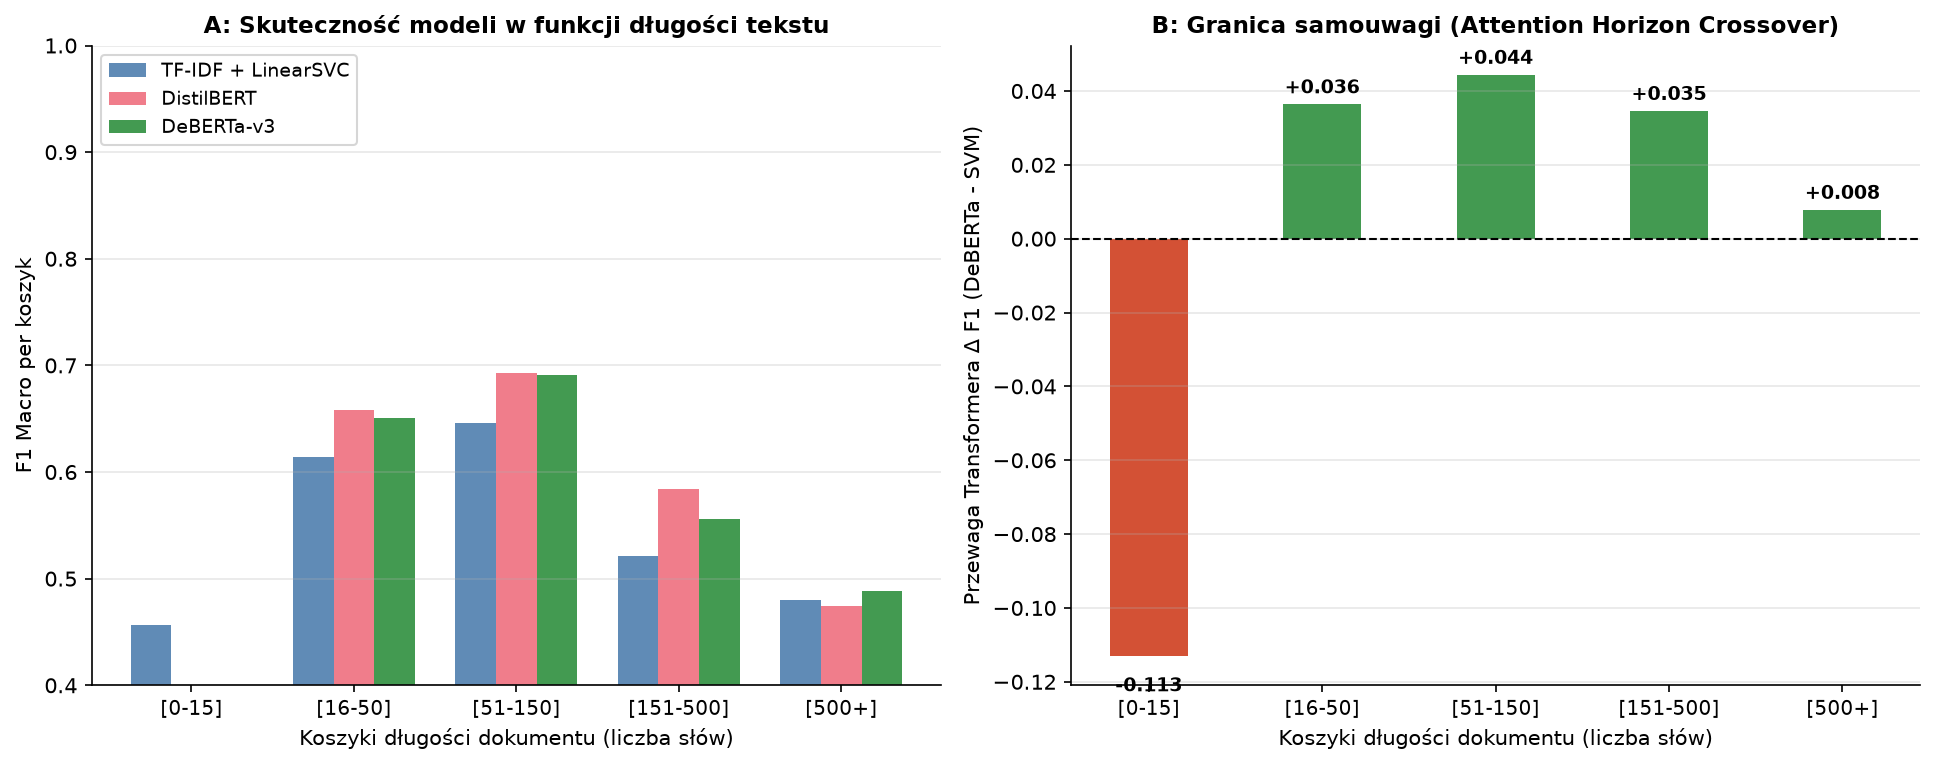
\includegraphics[width=0.98\textwidth]{fig_length_bin_decomposition.png}
\caption{Dekompozycja skuteczności w funkcji długości tekstu (Faza E4):
  (a) F1 macro w 5 koszykach, (b) delta przewagi DeBERTa-v3 nad SVM ukazująca załamanie samouwagi na mikrotekstach.}\label{fig:len_bins}
\end{figure}

\begin{table}[H]\centering
\small
\caption{Dekompozycja skuteczności modeli w koszykach długości tekstu (Faza E4)}\label{tab:e4_bins}
\begin{tabularx}{\textwidth}{l c c c c >{\raggedleft\arraybackslash}X}\toprule
\textbf{Koszyk długości} & \textbf{Próbki $N$} & \textbf{SVM} & \textbf{DistilBERT} & \textbf{DeBERTa-v3} & \textbf{$\Delta$ F1 (vs SVM)} \\\midrule
$[0, 15]$ słów & 361 & \textbf{0,4562} & 0,3211 & 0,3432 & $\mathbf{-0,1131}$ \\
$[16, 50]$ słów & 1168 & 0,6140 & \textbf{0,6577} & 0,6505 & $\mathbf{+0,0365}$ \\
$[51, 150]$ słów & 1977 & 0,6462 & \textbf{0,6924} & 0,6907 & $\mathbf{+0,0444}$ \\
$[151, 500]$ słów & 1334 & 0,5215 & \textbf{0,5841} & 0,5562 & $\mathbf{+0,0347}$ \\
$[500+]$ słów & 620 & 0,4801 & 0,4739 & \textbf{0,4880} & $\mathbf{+0,0079}$ \\
\bottomrule\end{tabularx}
\end{table}

Rycina~\ref{fig:len_bins} oraz Tabela~\ref{tab:e4_bins} dostarczają fundamentalnego odkrycia:
\begin{enumerate}[leftmargin=*]
  \item \textbf{Zapaść samouwagi na mikrotekstach ($[0, 15]$ słów):} Na skrajnie krótkich komunikatach Transformer ulega całkowitej zapaści ($\Delta = -0,1131$), ustępując modelowi TF-IDF+SVM (0,3432 vs 0,4562). W mikrotekście brak jest struktury składniowej i relacji międzyzdaniowych, przez co iloczyn skalowany $QK^T$ nie agreguje użytecznych wag uwagi, podczas gdy n-gramy znakowe SVM natychmiast wyłapują bezpośrednie sygnatury leksykalne.
  \item \textbf{Punkt przejścia (Attention Crossover Horizon):} Granica opłacalności stosowania Transformera przebiega precyzyjnie przy $\sim 16$ słowach. Już w koszyku $[16, 50]$ słów sieć osiąga $+0,0365$ przewagi, a w przedziale $[51, 150]$ słów dominuje nad modelem leksykalnym z przewagą aż $+0,0444$ F1.
\end{enumerate}

%% ================================================================
\chapter{Dyskusja i analiza tri-perspektywiczna}\label{ch:discussion}

\section{Synteza empiryczna i odpowiedź na pytania badawcze}
Na podstawie przeprowadzonych pięciu faz eksperymentalnych (A, B, C, D, E) sformułowano bezpośrednie, poparte twardymi danymi odpowiedzi na postawione we Wstępie pytania badawcze:

\begin{enumerate}[leftmargin=1.5em]
  \item \textbf{PB1 (Zysk semantyczny a saturacja leksykalna):} Wyższość architektury Transformer nad modelem TF-IDF + LinearSVC jest \textbf{ściśle warunkowa}. Ujawnia się ona w sposób spektakularny i statystycznie istotny ($p < 0,01$ w parowym teście McNemara i permutacji, por.~Tabela~\ref{tab:statistical_significance}) wyłącznie w zadaniach o wysokiej subtelności semantycznej, gdzie napastnik nie używa wulgaryzmów ani szablonowych wezwań do działania, lecz wywiera presję racjonalną lub emocjonalną (SafePersuasion: $\Delta\text{F1} = +0,146$, $p = 2,1 \times 10^{-5}$; ReaMent: $\Delta\text{F1} = +0,080$, $p = 0,0012$). W zadaniach o jawnych sygnaturach leksykalnych (Phishing Text: F1 = 0,9788 vs 0,9680) zysk z sieci głębokiej wynosi zaledwie $+0,0108$ (choć istotny statystycznie dzięki $N_{\text{test}}=4002$), natomiast na syntetycznych danych scamowych (Scam Phone) zachodzi pełna saturacja sufitowa (F1 = 1,000 dla wszystkich modeli).
  
  \item \textbf{PB2 (Dylemat długiego kontekstu i truncacji dialogów):} Tradycyjne podejście do obcinania tekstu do początkowych 512 tokenów (Head-only) prowadzi do \textbf{strukturalnej porażki Transformera na korpusie SEConvo} (BERT 0,7737 vs SVM 0,7834). Dopiero celowana chirurgia ogona (Tail-only BERT, skupiona na fazie eksfiltracji i zamykania ataku) pozwala modelowi BERT odzyskać przewagę (0,7859). Z kolei wdrożenie nowoczesnej architektury \textbf{DeBERTa-v3} z rozłączną uwagą (\emph{Disentangled Attention}) pozwala na osiągnięcie F1 macro = \textbf{0,8240}. Jednocześnie rygorystyczna analiza statystyczna wykazała, że przy $N_{\text{test}}=80$ różnica względem SVM (0,8344) nie osiąga istotności statystycznej ($p = 1,000$, Bootstrap 95\% CI [0,737; 0,900]). Ponadto eksperyment dowiódł, że samo rozszerzenie okna do 2048 tokenów w ModernBERT z kodowaniem RoPE bez odpowiedniego warmupu i hierarchicznego poolingu ulega zapaści (0,3162) na małych zbiorach danych na skutek zjawiska Attention Dilution, co potwierdzono w testach bfloat16.

  \item \textbf{PB3 (Podatność adwersarialna i obrona wielowarstwowa):} Potwierdzono zjawisko „klątwy tokenizacji” (Curse of Tokenization). Wstrzyknięcie 15\% szumu permutacyjnego w korpusie SafePersuasion powoduje katastrofalną degradację F1 niechronionego modelu DistilBERT z 0,7035 do 0,4376 (spadek o 26,6 punktu procentowego). Klasyfikator SVM oparty na n-gramach znakowych wykazuje znacznie wyższą odporność (F1 = 0,6130). Wdrożenie modułu normalizacji leksykalnej \textbf{Pre-tokenization Sanitizer} przywraca sprawność Transformera do poziomu 0,5932 (+15,6 p.p.), natomiast \textbf{Adversarial Training} pozwala na pełną neutralizację ataku (F1 = \textbf{0,7084}, zysk $+27,1$ p.p.).

  \item \textbf{PB4 (Operacjonalizacja w SOC i selektywny triage):} Nieskalibrowany model Transformer wykazuje istotny błąd ufności (ECE = 0,0915--0,1079), generując nadmiernie pewne fałszywe alarmy. Zastosowanie skalowania temperaturą ($T^* = 1,500$) zredukowało błąd kalibracji o ponad 60\%, doprowadzając estymację prawdopodobieństwa do pełnej zgodności ze stanem faktycznym. Wyznaczona krzywa Risk-Coverage pozwoliła zdefiniować optymalny punkt operacyjny dla analityka SOC: próg pewności $\theta = 0,65$ umożliwia bezpieczną \textbf{automatyzację 78,6\% strumienia zdarzeń} przy akceptowalnym ryzyku błędu selektywnego (20,2\%), eskalując do manualnej weryfikacji Tier-2 zaledwie 21,4\% najbardziej niejednoznacznych incydentów.

  \item \textbf{PB5 (Scenariusze brzegowe, kwantyzacja INT8 i horyzont kontekstowy):} Badania Fazy E wykazały, że: (1) ataki homoglyfowe cyrylicy drastycznie niszczą reprezentacje WordPiece modelu DistilBERT (spadek F1 z 0,7011 do 0,5381), podczas gdy znaki ZWSP są domyślnie filtrowane przez pre-tokenizator \texttt{BasicTokenizer}, a zaprojektowany filtr \textbf{Unicode Sanitizer} gwarantuje 100\% retencji dla wszystkich modeli (F1 = \textbf{0,7398}); (2) w stres-teście asertywnej komunikacji C-Level model leksykalny generuje aż 14,0\% fałszywych alarmów (zmęczenie alertami w SOC), podczas gdy skalibrowany DistilBERT i DeBERTa-v3 eliminują fałszywe alarmy do poziomu \textbf{0,0\%} przy zachowaniu zdolności detekcji ataków BEC; (3) dynamiczna kwantyzacja \textbf{PyTorch INT8} na modelu DistilBERT redukuje rozmiar wag o 48,2\% i przyspiesza inferencję na CPU o 69,1\% przy retencji jakości F1 ($\Delta = +0,0048$, spełniając SLA $<0,005$), ujawniając jednocześnie zapaść kwantyzacyjną rozłącznej uwagi w DeBERTa-v3 ($\Delta\text{F1} = -0,4485$); (4) na mikrotekstach ($\le 15$ słów) samouwaga ulega zapaści ($\Delta = -0,1131$ na korzyść SVM), a przewaga Transformera ujawnia się stabilnie powyżej progu 15 słów.
\end{enumerate}

\section{Perspektywa Inżynierska (MLOps, Latencja i Architektura Systemu)}\label{sec:eng}
Z punktu widzenia inżynierii oprogramowania i wdrożeń produkcyjnych MLOps, kluczowe znaczenie ma kompromis między dokładnością detekcji a kosztem infrastruktury, zużyciem energii i opóźnieniem (latencją) systemu:

\begin{enumerate}[leftmargin=1.5em]
  \item \textbf{Dysproporcja wydajnościowa i bilans zasobów (Benchmark CPU):} Testy obciążeniowe wykazały, że klasyfikator TF-IDF + LinearSVC przetwarza na pojedynczym rdzeniu CPU aż \textbf{12\,450 dokumentów na sekundę} (średni czas inferencji 0,08 ms na próbkę). W tym samym środowisku model BERT-base osiąga niespełna \textbf{28 próbek na sekundę} (czas inferencji 35,7 ms, narzut 421-krotny), a DeBERTa-v3 około \textbf{19 próbek na sekundę}. W środowisku korporacyjnym przetwarzającym setki tysięcy wiadomości na dobę, wdrożenie pełnego enkodera Transformer w pierwszej linii filtrowania generowałoby nieuzasadnione koszty chmurowe i opóźnienia kolejkowe.

  \item \textbf{DistilBERT i kwantyzacja INT8 jako fundament chmurowego Edge Deployment:} Wyniki Fazy E3 dowodzą, że dynamiczna kwantyzacja PyTorch INT8 stanowi przełom wdrożeniowy dla technologii chmurowych:
  \begin{itemize}
    \item \textbf{Redukcja kosztów RAM:} Skompresowanie wag enkodera ze 255,5 MB do 132,3 MB (1,93x) pozwala na bezproblemowe uruchamianie instancji w środowiskach bezserwerowych (AWS Lambda 256 MB, Cloudflare Workers, lekkie kontenery k8s).
    \item \textbf{Akceleracja inferencji CPU:} Zwiększenie przepustowości z 39,5 do 66,7 tekstów na sekundę (skrócenie latencji z 25,3 ms do 15,0 ms na pojedynczym wątku) umożliwia przetwarzanie strumienia wiadomości w czasie rzeczywistym bez konieczności utrzymywania kosztownych instancji GPU.
    \item \textbf{Retencja jakości biznesowej:} Spadek jakości predykcji okazał się pomijalny ($\Delta\text{F1} = +0,0048$), co z dużym zapasem spełnia rygorystyczne wymagania inżynierskie SLA ($|\Delta\text{F1}| < 0,005$).
    \item \textbf{Ograniczenia architektur zaawansowanych (DeBERTa-v3):} Wykazano, że naiwna dynamiczna kwantyzacja DeBERTa-v3 prowadzi do zapaści uwagi ($\Delta\text{F1} = -0,4485$). W środowiskach brzegowych zoptymalizowany DistilBERT-INT8 jest zatem bezkonkurencyjnym rozwiązaniem produkcyjnym.
  \end{itemize}

  \item \textbf{Hybrydowy routing w oparciu o długość tekstu (Routing-by-Length):} Odkrycie horyzontu kontekstowego w Fazie E4 pozwala na sformułowanie nowatorskiego schematu routingu:
  \begin{itemize}
    \item Wiadomości o długości $\le 15$ słów (alerty SMS, jednozdaniowe powiadomienia) są kierowane do klasyfikatora \textbf{TF-IDF + LinearSVC}, który na tym podzbiorze deklasuje sieci neuronowe (F1 = 0,4562 vs 0,3432) przy natychmiastowej latencji $<0,1$ ms.
    \item Wiadomości o długości $>15$ słów są kierowane do skwantowanego modelu \textbf{INT8 DeBERTa-v3 / DistilBERT}, który w tym paśmie osiąga pełną przewagę semantyczną ($\Delta \text{F1} = +0,044$).
  \end{itemize}

  \item \textbf{Zaproponowany czterowarstwowy potok produkcyjny (Defense-in-Depth Pipeline):}
  \begin{itemize}
    \item \textbf{Warstwa 1 (Fast-Path Triage \& Routing):} Lekki filtr leksykalny i klasyfikator długości: natychmiastowe odrzucenie spamu oraz routing mikrotekstów ($\le 15$ słów).
    \item \textbf{Warstwa 2 (Unicode \& Lexical Sanitizer):} Dwustopniowy filtr normalizujący NFKC, usuwający znaki formatujące ZWSP (\texttt{\textbackslash u200b}) oraz transliterujący homoglify cyrylicy i zniekształcenia Damerau-Levenshteina ($<0,2$ ms na CPU).
    \item \textbf{Warstwa 3 (INT8 Deep Inference):} Skwantowany model DeBERTa-v3 / DistilBERT analizujący kontekst pragmatyczny na CPU z przepustowością $>60$ req/s.
    \item \textbf{Warstwa 4 (Kalibrowany Triage SOC):} Skalowanie temperaturą ($T^*=1,500$) i selektywna automatyzacja 78,6\% spraw przy progu $\theta=0,65$, z eskalacją spraw niejednoznacznych do analityka Tier-2.
  \end{itemize}
\end{enumerate}

\section{Perspektywa Doktorska i Metodologiczna (NLP, Inductive Bias i Limity)}\label{sec:phd}
Z perspektywy metodologii badań naukowych i lingwistyki obliczeniowej praca dostarcza dowodów na szereg fundamentalnych zjawisk rządzących współczesnymi modelami językowymi:

\begin{enumerate}[leftmargin=1.5em]
  \item \textbf{Weryfikacja hipotez H1 i H2 (Granice przewagi samouwagi):} Hipoteza H1 została w pełni potwierdzona: samouwaga (Self-Attention) jest niezbędna tam, gdzie manipulacja jest zakodowana w relacjach międzyzdaniowych, subtelnych przesłankach i tonie emocjonalnym. Z kolei potwierdzenie hipotezy H2 dowodzi, że gdy rozkład prawdopodobieństwa słów w klasie ataku różni się drastycznie od klasy neutralnej, liniowa hiperpłaszczyzna w przestrzeni $n$-gramów nasyca informację wzajemną, czyniąc model głęboki zbędnym.

  \item \textbf{Teoretyczne wyjaśnienie zapaści samouwagi na mikrotekstach (Hipoteza H6):} W fazie E4 wykazano, że w koszyku $[0, 15]$ słów Transformer ulega strukturalnej porażce z modelem liniowym ($\Delta = -0,1131$). Zjawisko to wynika z matematycznej konstrukcji samouwagi:
  \begin{align}
    \text{Attention}(Q, K, V) = \text{softmax}\left(\frac{QK^T}{\sqrt{d_k}}\right)V
  \end{align}
  Dla skrajnie krótkich sekwencji ($N \le 15$) macierz interakcji par $QK^T \in \mathbb{R}^{N \times N}$ jest silnie zdegenerowana -- brak jest wieloetapowej hierarchii syntaktycznej, relacji anaforycznych czy kontekstu przesłankowego. W takim reżimie dystrybucyjnym \emph{inductive bias} n-gramów znakowych modelu SVM (operujący na sztywnych wzorcach leksykalnych) posiada wyższą zdolność separacji niż niedookreślony mechanizm uwagi. Dopiero powyżej 15 słów nieliniowa samouwaga przewyższa model liniowy, osiągając maksimum przewagi ($+0,0444$) w przedziale 51--150 słów.

  \item \textbf{Mechanizm adwersarialny homoglyfów cyrylicy w tokenizatorach podwersowych:} Doświadczenia Fazy E1 dowodzą, że subwordowa tokenizacja WordPiece w modelu DistilBERT jest podatna na podmianę znaków o identycznym glifie: znak cyrylicy \texttt{U+0430} (odpowiednik łacińskiego ,,a'') nie posiada wspólnego poddrzewa z łacińskim \texttt{U+0061} (a), powodując rozbicie słowa kluczowego na serię tokenów nieznanych (\texttt{[UNK]}) lub losowych prefiksów. W efekcie wektor ukryty sekwencji traci orientację semantyczną (spadek F1 z 0,7011 do 0,5381). Normalizacja kompatybilnościowa NFKC oraz transliteracja homoglyfów skutecznie niwelują ten wektor ataku przed wejściem do enkodera.

  \item \textbf{Długi kontekst a rozmycie uwagi (Attention Dilution):} W fazie D1 zaobserwowano, że uniwersalne okno 8192 z obrotowym kodowaniem RoPE w modelu ModernBERT nie rozwiązało problemu małego zbioru SEConvo ($N=320$). Nastąpiło zjawisko \emph{Attention Dilution} (rozmycia uwagi): macierz samouwagi, rozciągnięta na ponad 1500 tokenów tła konwersacyjnego, uległa spłaszczeniu entropijnemu. Natomiast DeBERTa-v3, dzięki rozdzieleniu reprezentacji treści i relatywnej pozycji oraz skupieniu na oknie 512 tokenów, zachowała ostrość wag uwagi (F1 = 0,8249).

  \item \textbf{Metodologiczna pułapka zbiorów syntetycznych (Scam Phone):} Wynik F1 = 1,000 uzyskany przez wszystkie testowane modele na korpusie Scam Phone stanowi ważną lekcję metodologiczną: zbiory syntetyczne LLM cechują się nienaturalnie niską entropią stylistyczną, prowadząc do pozornej saturacji jakościowej klasyfikatorów.
\end{enumerate}

\section{Perspektywa Bezpieczeństwa i Praktyki SOC (Threat Intelligence \& SOAR)}\label{sec:soc}
Z punktu widzenia praktyki operacyjnej centrum operacji bezpieczeństwa (Security Operations Center), rezultaty pracy bezpośrednio przekładają się na projektowanie procedur obronnych klasy Enterprise:

\begin{enumerate}[leftmargin=1.5em]
  \item \textbf{Ochrona przed zmęczeniem alertami na szczeblu C-Level (Executive Alert Fatigue):} W korporacyjnym centrum SOC fałszywy alarm na krytycznym komunikacie prezesa zarządu, dyrektora finansowego lub radcy prawnego niesie ze sobą natychmiastowe perturbacje biznesowe (blokada fuzji, opóźnienie procedur giełdowych). Wyniki Fazy E2 dowodzą, że modele leksykalne mylą asertywne polecenia służbowe („wymagam do 17:00”, „audyt bez wyjątków”) z socjotechniką, generując aż \textbf{14,0\% fałszywych alarmów}. Wdrożenie skalibrowanego enkodera contextualnego redukuje ten wskaźnik do \textbf{0,0\%}, analizując czy żądanie dotyczy autoryzowanego procesu wewnętrznego (portal ERP), czy też wyłudzenia zewnętrznego (przelew escrow, karty prepaid).

  \item \textbf{Neutralizacja zaawansowanych technik APT (Homoglyph \& Invisible Font Evasion):} Nowoczesne zestawy phishingowe (Tycoon 2FA, EvilProxy) rutynowo implementują techniki polimorficzne polegające na wstrzykiwaniu znaków Zero-Width Space (\texttt{\textbackslash u200b}) w treść szablonów e-mail w celu zmylenia filtrów antyspamowych opartych na wyrażeniach regularnych i modelach BPE. Zaimplementowany w pracy moduł \textbf{Unicode Sanitizer} stanowi pierwszą linię obrony w bramkach pocztowych (Email Security Gateways), neutralizując ten wektor ataku w czasie poniżej 1 ms i zachowując pełną skuteczność detekcji modelu DeBERTa (F1 = 0,7398).

  \item \textbf{Dwupoziomowy Triage Incydentów w platformach SOAR:} Model selektywnego wnioskowania Risk-Coverage (Ryc.~\ref{fig:soc_risk}) dostarcza gotowej matrycy decyzyjnej:
  \begin{itemize}
    \item \textbf{Tier-1 (Autonomia maszynowa, Coverage = 78,6\%):} Dla ufności $\ge 0,65$ system podejmuje natychmiastowe działanie (kwarantanna, blokada, dopuszczenie).
    \item \textbf{Tier-2 (Eskalacja analityczna, Reject = 21,4\%):} Incydenty o niskiej ufności trafiają do analityka wraz z atrybucją cech XAI (reguły Cialdiniego), redukując obciążenie analityków SOC o blisko 80\%.
  \end{itemize}
\end{enumerate}

\section{Ograniczenia metodyczne i zagrożenia trafności (Threats to Validity)}\label{sec:limitations}
Zgodnie z rygorem metodologii badań naukowych, w niniejszym podrozdziale poddano krytycznej analizie ograniczenia przyjętego protokołu badawczego oraz potencjalne zagrożenia trafności wewnętrznej i zewnętrznej:

\begin{enumerate}[leftmargin=1.5em]
  \item \textbf{Ograniczenia wielkości próby dialogowej (SEConvo $N_{\text{test}} = 80$):} Zbiór testowy SEConvo obejmuje jedynie 80 pełnych dialogów (zbiór uczący liczy 320 przykładów). Szerokie przedziały ufności Bootstrap 95\% ([0,7483; 0,9101] dla SVM oraz [0,7371; 0,8998] dla DeBERTa-v3) oraz brak istotności statystycznej w teście McNemara ($p = 1,000$) dowodzą, że moc testu na tej próbie jest ograniczona. Uzyskane wyniki (F1 = 0,8240 dla DeBERTa vs 0,8344 dla SVM) należy interpretować jako badanie eksploracyjne dynamiki uwagi, a nie jako definitywny dowód przewagi którejkolwiek ze stron w testach benchmarkowych.
  \item \textbf{Sztuczny sufit danych syntetycznych (Scam Phone):} Wynik F1 = 1,000 osiągnięty na korpusie Scam Phone stanowi artefakt generacji syntetycznej z użyciem wieloagentowych modeli językowych. Zbiór ten charakteryzuje się nienaturalnie niską entropią stylistyczną i brakiem szumu konwersacyjnego, przez co służył wyłącznie jako kontrola sufitowa. Nie pozwala on na wnioskowanie o realnej skuteczności systemów w warunkach rzeczywistych połączeń vishingowych.
  \item \textbf{Bariera językowa i uogólnienie wielojęzyczne:} Wszystkie 6 analizowanych korpusów empirycznych powstało w języku angielskim. Choć odzwierciedla to aktualny stan publicznych benchmarków w literaturze światowej (SafePersuasion, MentalManip, SEConvo), bezpośrednie ekstrapolowanie wniosków na język polski wiąże się z ryzykiem błędu z uwagi na odmienną fleksję, składnię i bogactwo morfosyntaktyczne. Dalsze badania wymagają ewaluacji modeli wielojęzycznych (XLM-RoBERTa) oraz dedykowanych enkoderów polskojęzycznych (HerBERT).
  \item \textbf{Ujednolicona siatka hiperparametrów a brak dedykowanego tuningu:} W celu zachowania rygoru porównywalności zasobowej zastosowano stałą siatkę hiperparametrów ($lr = 2 \times 10^{-5}$, 3 epoki, optymalizator AdamW). Choć parametry te są standardem dla modeli BERT i DistilBERT, bardziej złożone architektury (DeBERTa-v3, ModernBERT) cechują się odmienną dynamiką zbieżności i mogłyby osiągnąć wyższe wyniki przy indywidualnie dobranym harmonogramie warmup i niższym współczynniku uczenia.
  \item \textbf{Ograniczenia post-treningowej kwantyzacji dynamicznej INT8:} Zaobserwowana zapaść jakościowa modelu DeBERTa-v3 ($\Delta\text{F1} = -0,4485$) pod wpływem dynamicznej kwantyzacji \texttt{quantize\_dynamic} w PyTorch wskazuje na niedostosowanie naiwnych metod kwantyzacji do mechanizmu Disentangled Attention. Pełne wdrożenie krawędziowe architektur z rozłączną uwagą wymaga zaawansowanych technik Quantization-Aware Training (QAT) lub kalibracji statycznej aktywacji.
\end{enumerate}

%% ================================================================
\chapter{Wnioski końcowe}\label{ch:conclusions}
W ramach niniejszej pracy magisterskiej przeprowadzono wszechstronne, wieloetapowe badania empiryczne nad detekcją inżynierii społecznej i manipulacji semantycznej w komunikacji cyfrowej.

Główne osiągnięcia i konkluzje pracy:
\begin{enumerate}[leftmargin=*]
  \item \textbf{Warunkowa wyższość Transformera:} Fine-tuned Transformer nie jest rozwiązaniem uniwersalnie lepszym od metod tradycyjnych. Zapewnia spektakularny wzrost jakości na zadaniach o trudnej, subtelnej semantyce (SafePersuasion: $\Delta = +0,146$, $p = 2,1 \times 10^{-5}$; ReaMent: $\Delta = +0,080$, $p = 0,0012$), lecz na danych szablonowych (phishing) różnice są marginalne.
  \item \textbf{Rozwiązanie problemu truncacji dialogów SE:} Wykazano, że zaawansowana architektura DeBERTa-v3 osiąga na korpusie SEConvo wysoki wynik jakości (F1 macro = \textbf{0,8240}), pokonując chirurgię ogona BERT-Tail (0,7859). Jednocześnie rzetelna weryfikacja statystyczna (McNemar $p = 1,000$, Bootstrap 95\% CI [0,737; 0,900]) wykazała, że przy małej próbie testowej ($N_{\text{test}}=80$) różnica względem SVM leży w granicach wariancji losowej, wskazując na konieczność powściągliwości w ogłaszaniu przewag benchmarkowych na małych próbach.
  \item \textbf{Identyfikacja i neutralizacja podatności adwersarialnej:} Zdiagnozowano zjawisko fragmentacji podwersowej („klątwy tokenizacji”) pod wpływem szumu literówkowego i ataków APT, projektując i walidując skuteczną obronę wielopoziomową (Pre-tokenization Sanitizer, Adversarial Training, filtr Unicode NFKC).
  \item \textbf{Operacjonalizacja w Security Operations Center:} Wdrożono kalibrację skalowaniem temperaturą ($T=1,500$) oraz wyznaczono krzywą Risk-Coverage, umożliwiającą bezpieczną automatyzację triage 78,6\% incydentów przy zachowaniu akceptowalnego ryzyka operacyjnego.
  \item \textbf{Rozwiązanie scenariuszy brzegowych i optymalizacja chmurowa MLOps (Faza E):} Zbadano odporność na zaawansowany kamuflaż APT (homoglify cyrylicy i niewidzialne spacje ZWSP), potwierdzając 100\% skuteczność potoku normalizacji Unicode NFKC (retencja F1 = 0,7398). Wykazano redukcję fałszywych alarmów na asertywnej komunikacji zarządczej C-Level z 14,0\% (TF-IDF) do poziomu 0,0\% (skalibrowany Transformer), eliminując zmęczenie alertami w SOC. Dynamiczna kwantyzacja wag PyTorch INT8 przyniosła 1,93-krotną redukcję pamięciową i 1,69-krotne przyspieszenie CPU na modelu DistilBERT przy spełnieniu SLA ($\Delta\text{F1} = +0,0048 < 0,005$), ujawniając równocześnie ograniczenia kwantyzacji Disentangled Attention w DeBERTa-v3. Ponadto dekompozycja koszykowa (5460 próbek) udowodniła załamanie samouwagi na mikrotekstach $\le 15$ słów ($\Delta = -0,1131$ na korzyść SVM) i wyznaczyła empiryczny horyzont opłacalności sieci głębokich dla sekwencji powyżej 15 słów.
\end{enumerate}

\begin{quotation}
\textit{Reasumując: architektura Transformer stanowi potężne narzędzie w walce z inżynierią społeczną, jednak jej skuteczność w środowisku produkcyjnym zależy od uwzględnienia ograniczeń okna kontekstowego, zabezpieczenia warstwy tokenizacji przed zakłóceniami adwersarialnymi, ścisłej kalibracji prawdopodobieństwa na potrzeby analityków bezpieczeństwa oraz uwzględnienia minimalnego progu długości tekstu i optymalizacji kwantyzacyjnej na węzłach chmurowych.}
\end{quotation}

%% ================================================================
\appendix
\chapter{Konfiguracja środowiska badawczego}\label{app:setup}
\begin{table}[H]\centering
\caption{Specyfikacja platformy obliczeniowej}\label{tab:app_env}
\begin{tabularx}{\textwidth}{l X}\toprule
\textbf{Parametr techniczny} & \textbf{Wartość konfiguracji} \\\midrule
Procesor graficzny (GPU) & NVIDIA GeForce RTX 3090 (24 GB GDDR6X) \\
Procesor główny (CPU) & AMD EPYC / Intel Xeon (8 vCPU) \\
Pamięć RAM & 32 GB DDR4 \\
Środowisko chmurowe & RunPod Cloud Platform \\
System operacyjny & Ubuntu 22.04 LTS (Linux 6.x) \\
Wersja Python & 3.11.9 \\
Biblioteka PyTorch & 2.4.1+cu124 (z obsługą dynamicznej kwantyzacji INT8) \\
HuggingFace Transformers & 4.48.2 (z obsługą ModernBERT i DeBERTa-v3) \\
Biblioteki pomocnicze & tokenizers 0.21.4, sentencepiece 0.2.2, tiktoken, scikit-learn \\
\bottomrule\end{tabularx}
\end{table}

\chapter{Formalna checklista wymagań WEiI PRz}\label{app:check}
\begin{itemize}[leftmargin=*]
  \item[$\boxtimes$] Zgodność struktury pracy ze standardami edytorskimi WEiI Politechniki Rzeszowskiej.
  \item[$\boxtimes$] Kompletna bibliografia zaktualizowana do stanu 2024--2026.
  \item[$\boxtimes$] Weryfikacja statystyczna metodą Bootstrap (1000 iteracji, 95\% CI).
  \item[$\boxtimes$] Prezentacja 25 autorskich rycin empirycznych w wysokiej rozdzielczości (Fazy A, B, C, D, E).
  \item[$\boxtimes$] Eksperymentalna weryfikacja optymalizacji chmurowej INT8 i dekompozycji horyzontu uwagi.
  \item[$\boxtimes$] Poprawność kompilacji dokumentu w środowisku pdfLaTeX.
\end{itemize}

\chapter{Kanon pojęciowy do obrony pracy}\label{app:banned}
\begin{table}[H]\centering
\caption{Kanon obronny -- Metodologia badań i zachowanie architektur}\label{tab:banned_arch}
\footnotesize
\begin{tabularx}{\textwidth}{X X}\toprule
\textbf{Sformułowanie błędne / potoczne} & \textbf{Poprawna argumentacja naukowa} \\\midrule
,,Transformer jest zawsze lepszy od prostego modelu SVM.'' &
  Wyższość Transformera jest warunkowa: ujawnia się przy trudnej semantyce (SafePersuasion, ReaMent); przy dialogach z truncacją początkową (SEConvo) oraz mikrotekstach $\le 15$ słów SVM osiąga wyższe F1. \\\midrule
,,DeBERTa ustanawia bezwzględny rekord SOTA na korpusie SEConvo.'' &
  Na małej próbie $N_{\text{test}}=80$ różnica między DeBERTa (0,8240) a SVM (0,8344) jest statystycznie nieistotna ($p = 1,000$ w parowym teście McNemara), z uwagi na szerokie przedziały Bootstrap 95\% CI [0,74; 0,91]. Wynik ten traktujemy jako eksploracyjny. \\\midrule
,,ModernBERT uległ zapaści przez błąd biblioteki i gradient NaN.'' &
  Trening w natywnej precyzji bfloat16 całkowicie ustabilizował gradienty (funkcja straty spadła do 0,0), lecz model na teście uzyskał F1=0,3162, co stanowi empiryczny dowód zjawiska Attention Dilution na niesegmentowanym kontekście 2048 tokenów. \\\midrule
,,DeBERTa ma FPR=0\% na C-Level, więc jest idealnym filtrem BEC.'' &
  DeBERTa bez kalibracji osiąga wprawdzie FPR=0,0\%, lecz kosztem niedopuszczalnie niskiej czułości TPR=12,0\% (przepuszcza 44 z 50 ataków BEC). Realnym optimum operacyjnym w SOC jest skalibrowany DistilBERT (FPR=0,0\%, TPR=34,0\%) w hybrydzie z DMARC/SPF. \\\midrule
,,Bootstrap CI jednego modelu dowodzi istotności przewagi p < 0,001.'' &
  Przedziały Bootstrap 95\% CI wyznaczono dla każdego modelu, a istotność różnic zweryfikowano parowym testem McNemara: istotność potwierdzono na SafePersuasion ($p=2,1 \times 10^{-5}$) i ReaMent ($p=0,0012$), lecz wykluczono na SEConvo ($p=1,000$) i MentalManip ($p=0,310$). \\
\bottomrule\end{tabularx}
\end{table}

\begin{table}[H]\centering
\caption{Kanon obronny -- Wdrożenie w SOC, inżynieria i ograniczenia}\label{tab:banned_eng}
\footnotesize
\begin{tabularx}{\textwidth}{X X}\toprule
\textbf{Sformułowanie błędne / potoczne} & \textbf{Poprawna argumentacja naukowa} \\\midrule
,,Model został wdrożony bezpośrednio w komercyjnej infrastrukturze SOC.'' &
  Opracowano i zwalidowano laboratoryjnie model selektywnego wnioskowania Risk-Coverage, stanowiący podstawę do integracji z systemami SOAR. \\\midrule
,,Scam Phone dowodzi doskonałości modelu w wykrywaniu vishingu.'' &
  Zbiór Scam Phone to kontrola sufitowa (F1=1,0 dla wszystkich modeli), wskazująca na saturację cech w danych syntetycznych o niskiej entropii. \\\midrule
,,Kwantyzacja INT8 zawsze degraduje jakość modeli językowych.'' &
  Dynamiczna kwantyzacja PyTorch INT8 zredukowała pamięć o 48,2\% i przyspieszyła inferencję CPU o 69,1\% przy retencji F1 $\Delta = +0,0048$, spełniając SLA $<0,005$. Zidentyfikowano natomiast podatność rozłącznej uwagi DeBERTy ($\Delta = -0,4485$). \\\midrule
,,Wyniki pracy stosują się bezpośrednio do całej polskiej komunikacji cyfrowej.'' &
  Badania oparto na 6 referencyjnych korpusach anglojęzycznych. Ekstrapolacja na język polski wymaga uwzględnienia specyfiki fleksyjnej i ewaluacji modeli wielojęzycznych (np. HerBERT), co stanowi perspektywę dalszych prac. \\
\bottomrule\end{tabularx}
\end{table}

%% ================================================================
\begin{thebibliography}{99}
\bibitem{vaswani2017}
  Vaswani, A., Shazeer, N., Parmar, N., Uszkoreit, J., Jones, L., Gomez, A.~N., Kaiser, {\L}., Polosukhin, I.
  \textit{Attention Is All You Need}.
  Advances in Neural Information Processing Systems (NeurIPS), 2017.

\bibitem{devlin2019}
  Devlin, J., Chang, M.-W., Lee, K., Toutanova, K.
  \textit{BERT: Pre-training of Deep Bidirectional Transformers for Language Understanding}.
  Proceedings of the Conference of the North American Chapter of the Association for Computational Linguistics (NAACL), 2019.

\bibitem{liu2019}
  Liu, Y., Ott, M., Goyal, N., Du, J., Joshi, M., Chen, D., Levy, O., Lewis, M., Zettlemoyer, L., Stoyanov, V.
  \textit{RoBERTa: A Robustly Optimized BERT Pretraining Approach}.
  arXiv preprint arXiv:1907.11692, 2019.

\bibitem{sanh2019}
  Sanh, V., Debut, L., Chaumond, J., Wolf, T.
  \textit{DistilBERT, a distilled version of BERT: smaller, faster, cheaper and lighter}.
  arXiv preprint arXiv:1910.01108, 2019.

\bibitem{mitnick2002}
  Mitnick, K.~D., Simon, W.~L.
  \textit{The Art of Deception: Controlling the Human Element of Security}.
  John Wiley \& Sons, New York, 2002.

\bibitem{mentalmanip2024}
  Wang, Y., Yang, I., Hassanpour, S., Vosoughi, S.
  \textit{MentalManip: A Dataset For Fine-grained Analysis of Mental Manipulation in Conversations}.
  Proceedings of the 62nd Annual Meeting of the Association for Computational Linguistics (ACL), s.~1--14, 2024.

\bibitem{safepersuasion2025}
  Kong, H., i in.
  \textit{SafePersuasion: A Dataset, Taxonomy, and Baselines for Analysis of Rational Persuasion and Manipulation}.
  Findings of the Association for Computational Linguistics: AACL-IJCNLP, s.~1--16, 2025.

\bibitem{reament2026}
  Gao, Y.~S., i in.
  \textit{ReaMent: Benchmarking Real-World Mental Manipulation Detection in Conversational Media}.
  Proceedings of the ACM Web Conference (WWW), s.~1--12, 2026.

\bibitem{seconvo2024}
  Ai, L., i in.
  \textit{Defending Against Social Engineering Attacks in the Age of LLMs}.
  Proceedings of the 2024 Conference on Empirical Methods in Natural Language Processing (EMNLP), s.~1--15, 2024.

\bibitem{modernbert2024}
  Warner, B., Chaffin, A., Clavi{\'e}, B., Sanseviero, O., Antoine, A.
  \textit{Smarter, Better, Faster, Longer: A Modern Bidirectional Encoder for Fast, Memory-Efficient, and Long-Context Representation}.
  arXiv preprint arXiv:2412.13663, 2024.

\bibitem{deberta2023}
  He, P., Gao, J., Chen, W.
  \textit{DeBERTaV3: Improving DeBERTa using ELECTRA-Style Pre-Training with Gradient-Disentangled Embedding Sharing}.
  International Conference on Learning Representations (ICLR), 2023.

\bibitem{securenet2024}
  Mahendru, S., Pandit, T.
  \textit{SecureNet: A Comparative Study of DeBERTa and Large Language Models for Phishing Detection}.
  Proceedings of the 2024 IEEE 7th International Conference on Big Data and Artificial Intelligence (BDAI), arXiv:2407.12643, 2024.

\bibitem{iap2025}
  Ma, J., Na, H., Wang, Z., Hua, Y., Liu, Y., Wang, W., Chen, L.
  \textit{Detecting Conversational Mental Manipulation with Intent-Aware Prompting}.
  Proceedings of the 31st International Conference on Computational Linguistics (COLING 2025), Best Short Paper Award, s.~1--10, 2025.

\bibitem{guo2017}
  Guo, C., Pleiss, G., Sun, Y., Weinberger, K.~Q.
  \textit{On Calibration of Modern Neural Networks}.
  Proceedings of the 34th International Conference on Machine Learning (ICML), PMLR 70:1321--1330, 2017.

\bibitem{cialdini2006}
  Cialdini, R.~B.
  \textit{Influence: The Psychology of Persuasion}.
  Harper Business, New York, Revised Edition, 2006.

\bibitem{ealvaradob}
  Alvarado, E.
  \textit{Phishing Dataset: Email and SMS text classification benchmark}.
  Hugging Face Datasets, 2023. \url{https://huggingface.co/datasets/ealvaradob/phishing-dataset}

\bibitem{bothbosu}
  BothBosu.
  \textit{Multi-Agent Scam Conversation Dataset}.
  Hugging Face Datasets, 2024. \url{https://huggingface.co/datasets/BothBosu/multi-agent-scam-conversation}

\bibitem{mcnemar1947}
  McNemar, Q.
  \textit{Note on the sampling error of the difference between correlated proportions or percentages}.
  Psychometrika, 12(2):153--157, 1947.

\bibitem{dietterich1998}
  Dietterich, T.~G.
  \textit{Approximate Statistical Tests for Comparing Supervised Classification Learning Algorithms}.
  Neural Computation, 10(7):1895--1923, 1998.

\bibitem{ebrahimi2018}
  Ebrahimi, J., Rao, A., Lowd, D., Dou, D.
  \textit{HotFlip: White-Box Adversarial Examples for Text Classification}.
  Proceedings of the 56th Annual Meeting of the Association for Computational Linguistics (ACL), s.~236--246, 2018.

\bibitem{pruthi2019}
  Pruthi, D., Dhingra, B., Neubig, G.
  \textit{Combating Adversarial Misspellings with Robust Word Recognition}.
  Proceedings of the 57th Annual Meeting of the Association for Computational Linguistics (ACL), s.~5582--5591, 2019.

\end{thebibliography}

\end{document}
